\begin{proposition}
Given an ideal propensity-model $p_{u, i}; \ \mathcal{I}_p(u, i ~|~ \mathcal{P})$ is an unbiased estimator of $\Delta(u, i ~|~ \mathcal{P})$.
\end{proposition}

\begin{proof}
\begin{align*}
    \EE_{u \sim \mathcal{U}} \EE_{i \sim \mathcal{I}} \left[ \mathcal{I}_p(u, i ~|~ \mathcal{P}) \right] \hspace{5.65cm}
\end{align*}
\vspace{-0.4cm}
\begin{align*}
    &= \frac{1}{|\mathcal{U}| |\mathcal{I}|} \sum_{u \sim \mathcal{U}} \sum_{i \sim \mathcal{I}} \mathcal{I}_p(u, i ~|~ \mathcal{P}) \cdot P(r_i^u = 1) \\
    % &= \frac{1}{|\mathcal{U}| \cdot |\mathcal{I}|} \sum_{u \sim \mathcal{U}} \sum_{i \sim \mathcal{I}} \mathcal{I}_p(u, i ~|~ \mathcal{P}) \cdot \left( P(r_i^u = 1, \overstar{r}_i^u = 0) ~+~ P(r_i^u = 1, \overstar{r}_i^u = 1) \right) \\
    &= \begin{aligned}[t]
        \frac{1}{|\mathcal{U}| |\mathcal{I}|} \sum_{u \sim \mathcal{U}} \sum_{i \sim \mathcal{I}} \frac{\Delta(u, i ~|~ \mathcal{P})}{p_{u, i}} \cdot ( P(\overstar{r}_i^u = 0) \cdot \cancelto{0}{P(r_i^u = 1 ~|~ \overstar{r}_i^u = 0)} \\
        +~ P(\overstar{r}_i^u = 1) \cdot P(r_i^u = 1 ~|~ \overstar{r}_i^u = 1)) \\ % \hspace{3.6cm} \\
        % \text{(One-sided label noise)} \\
    \end{aligned} \\
    &= \frac{1}{|\mathcal{U}| |\mathcal{I}|} \sum_{u \sim \mathcal{U}} \sum_{i \sim \mathcal{I}} \Delta(u, i ~|~ \mathcal{P}) \cdot P(\overstar{r}_i^u = 1) \\ %\hspace{0.5cm} 
    &= \EE_{u \sim \mathcal{U}} \EE_{i \sim \mathcal{I}} \left[ \Delta(u, i ~|~ \mathcal{P}) \right] \qedhere
\end{align*}
\end{proof}
\begin{table}[!ht]
    % \vspace{-1mm} %Put here to reduce too much white space after your table
    \begin{footnotesize} % normalsize, small, footnotesize
    \begin{center}
        \begin{tabular}{c | c c c c}
            \toprule
            \multirow{2}{*}{\textbf{Dataset}} & \textbf{\#} & \textbf{\#} & \textbf{\#} & \textbf{Avg. User} \\ 
            & \textbf{Interactions} & \textbf{Users} & \textbf{Items} & \textbf{history length} \\
            \midrule
            
            Amazon Magazine      & 12.7k & 3.1k  & 1.3k  & 4.1 \\
            ML-100k              & 100k  & 943   & 1.7k  & 106.04 \\
            Amazon Luxury        & 126k  & 29.7k & 8.4k  & 4.26 \\
            Amazon Video-games   & 973k  & 181k  & 55.3k & 5.37 \\
            BeerAdvocate         & 1.51M & 18.6k & 64.3k & 81.45 \\
            Goodreads Comics     & 4.37M & 133k  & 89k   & 32.72 \\
            
            \bottomrule
        \end{tabular}
    \end{center}
    \end{footnotesize}
    \vspace{2mm}
    \caption{Data statistics of the \emph{six} datasets used in this paper.}
    \label{data_stats}
    \vspace{-6mm} %Put here to reduce too much white space after your table
\end{table}
In this work, we discussed two approaches for representative sampling of CF-data, especially for accurately retaining the \emph{relative} performance of different recommendation algorithms. First, we proposed \sampler, which is better than commonly used sampling strategies, followed by introducing \oracle which \emph{analyzes} the performance of different samplers on different datasets. Detailed experiments suggest that \oracle can confidently estimate the downstream utility of any sampler within a few milliseconds, thereby enabling practitioners to benchmark different algorithms on $10$\% data sub-samples, with an average $5.8\times$ time speedup.

To realize the real-world environmental impact of \oracle, we discuss a typical weekly RecSys development cycle 
% in the industry 
and its carbon footprint. 
Taking the Criteo Ad dataset as inspiration, we assume a common industry-scale dataset to have $\sim4$B interactions.
% Inspired by the Criteo Ad Terabyte dataset, which is a collection of 24 days of ad-click logs, we assume a common industrial dataset to have around $4$ billion interactions. 
We assume a hypothetical use case that benchmarks for \eg $25$ different algorithms, each with $40$ different hyper-parameter variations. To estimate the energy consumption of GPUs, we scale the $0.4$ minute MLPerf \cite{mlperf} run of training NeuMF \cite{neural_mf} on the Movielens-20M dataset over an Nvidia DGX-2 machine. The total estimated run-time for all experiments would be $25 \times 40 \times \frac{4B}{20M} \times \frac{0.4}{60} \approx 1340$ hours; and following \cite{co2e}, the net CO$_2$ emissions would roughly be $10 \times 1340 \times 1.58 \times 0.954 \approx 20k$ lbs. To better understand the significance of this number, a brief CO$_2$ emissions comparison is presented in \cref{co2e}. Clearly, \oracle along with saving a large amount of experimentation time and cloud compute cost, can also significantly reduce the carbon footprint of this \emph{weekly process} by more than an average human's \emph{yearly} CO$_2$ emissions.

% \begin{wraptable}{r}{0.36\textwidth}
\begin{table}[!ht]
    \vspace{-5mm} %Put here to reduce too much white space after your table
    \begin{footnotesize} % normalsize, small, footnotesize
    \begin{center}
        \begin{tabular}{c c}
            \toprule
            \textbf{Consumption} & \textbf{CO$_2$e (lbs.)} \\ \midrule
            
            1 person, NY$\leftrightarrow$SF flight      & 2k \\
            Human life, 1 year avg.                     & 11k \\ 
            \midrule
            Weekly RecSys development cycle             & 20k \\
            '' \ \ \ \ \emph{w/} \oracle                & 3.4k \\
            
            \bottomrule
        \end{tabular}
    \end{center}
    \end{footnotesize}
    \vspace{2mm}
    \caption{CO$_2$ emissions comparison \cite{co2e}}
    % \caption*{Table 1: CO$_2$ emissions comparison}
    \label{co2e}
    \vspace{-10mm} %Put here to reduce too much white space after your table
\end{table}
% \end{wraptable}

Despite having significantly benefited the run-time and environmental impacts of benchmarking %recommendation 
algorithms on massive datasets, our analysis heavily relied on the experiments of training seven 
%different 
recommendation algorithms on six datasets and their various samples. Despite the already large experimental cost, we strongly believe that the downstream performance of \oracle could be further improved by simply 
% adding 
considering
more algorithms and diverse datasets.
% with different characteristics. 
In addition to better sampling, analyzing the fairness 
% and privacy 
aspects of training algorithms on sub-sampled datasets is an interesting research direction, which we plan to explore in future work.
% Future work: Fairness, SVP w/ sequential, New samplers
Although the results presented in \cref{main_exp} are indicative of correlation between the ranking of recommendation algorithms on the full dataset \vs smaller sub-samples, there still is no `one-size-fits-all' solution to the question of \emph{how to best sub-sample a dataset for retaining the performance of different recommendation algorithms?} In this section, we propose \oracle, that attempts to answer this question from a statistical perspective, in contrast with existing literature that generally has to resort to sensible heuristics \cite{large_graphs, scaling_up, sampling_cf_nn}.

\subsection{Problem formulation}
Given a dataset \dataset, we aim to gauge how a \emph{new} sampling strategy will perform in retaining the performance of different recommendation algorithms. Having already experimented with sixteen different sampling strategies on six datasets (\cref{main_exp}), we take a frequentist approach in predicting the performance of any sampling scheme. To be precise, to predict the performance of sampling scheme $s$ on dataset \dataset, we start by creating \dataset's subset according to $s$ and call it $\mathcal{D}^s$. We then represent \dataset and $\mathcal{D}^s$ in a low-dimensional latent space, followed by a powerful regression model to directly estimate the performance of $s$ on \dataset.

\subsection{Dataset representation} \label{data_rep}
We experiment with the following techniques of embedding a user-item interaction dataset into lower dimensions:

\subsubsection{Handcrafted. \ \ } For this method, we cherry-pick a few representative characteristics of \dataset and the underlying user-item bipartite interaction graph $\mathcal{G}$. Inspired by prior work \cite{large_graphs}, we represent \dataset as a combination of five features. We first utilize the frequency distribution of all users and items in \dataset. Next, we evaluate the distribution of the top$-100$ eigenvalues of $\mathcal{G}$'s adjacency matrix. All of these three distributions are generally long-tailed and heavily skewed. Furthermore, to capture notions like the diameter of $\mathcal{G}$, we compare the distribution of the number of hops $h$ \vs the number of pairs of nodes in $\mathcal{G}$ reachable at a distance less than $h$ \cite{hop_plot}. This distribution, unlike others is monotonically increasing in $h$. Finally, we also compute the size distribution of all connected components in $\mathcal{G}$, where a connected component is defined to be the maximal set of nodes, such that a path exists between any pair of nodes. Ultimately, we ascertain \dataset's final representation by concatenating $10$ evenly-spaced samples from each of the aforementioned distributions along with the total number of users, items, and interactions in \dataset. This results in a $53-$dimensional embedding for each dataset. Note that unlike previous work of simply \emph{retaining} the discussed features as a proxy of the quality of data subsets \cite{large_graphs}, \oracle instead uses these features to learn a regression model \emph{on-top} which can dynamically establish the importance of each feature in the performance of a sampling strategy.

\subsubsection{Unsupervised GCN. \ \ } With the recent advancements in the field of Graph Convolutional Networks \cite{original_gcn} to represent graph-structured data for a variety of downstream tasks, we also experiment with a GCN approach to embed $\mathcal{G}$. We modify the InfoGraph framework \cite{infograph}, which uses graph convolution encoders to obtain patch-level representations, followed by sort-pooling \cite{sort_pooling} to obtain a fixed, low-dimensional embedding for the entire graph. Since the nodes in $\mathcal{G}$ are the union of all users and items in \dataset, we randomly initialize $32-$dimensional embeddings using a Xavier-uniform prior \cite{xavier}. Parameter optimization is performed in an unsupervised fashion by maximizing the mutual information \cite{mutual_information} amongst the graph-level and patch-level representations of nodes in the same graph. We validate the best values of the latent dimension and number of layers of the GCN from $\{ 4, 8, 16, 32 \}$ and $\{ 1, 3 \}$ respectively.

\subsection{Training \& Inference} \label{oracle_architecture}
Having discussed different representation functions $\mathcal{E} : \mathcal{D} \mapsto \mathbb{R}^d$ to embed a CF-dataset in \cref{data_rep}, we now discuss \oracle's training framework agnostic to the actual details about $\mathcal{E}$. 

\paragraph{Optimization problem.} As a proxy of the performance of a sampler on a given dataset, we re-use the Kendall's Tau for each CF-scenario, metric, and sampling percent used while computing the $\Psi(\mathcal{D}, s)$ in \cref{main_exp}. To be specific, given $\mathcal{D}_{f}^{s, p}$ which is a $p\%$ sample of $f-$type feedback data $\mathcal{D}_f$, sampled according to sampling strategy $s$, we aim to estimate $\tau(\mathcal{R}_{f, m}, \mathcal{R}_{f, m}^{s, p})$ without ever computing the actual ranking of algorithms 
% $\mathcal{R}_{f, m}, \mathcal{R}_{f, m}^{s, p}$ 
on either the full or sampled datasets:
\begin{equation} \label{tau_hat}
    \hat{\tau}\left(\mathcal{R}_{f, m}, \mathcal{R}_{f, m}^{s, p}\right) = \Phi\left(\mathcal{E}(\mathcal{D}_f), \mathcal{E}(\mathcal{D}_f^{s, p}), m\right),
\end{equation}
where $\Phi$ is an arbitrary neural network, and $m$ is the metric of interest (see \cref{model_scenario_table}). We train $\Phi$ by either (1) regressing on the Kendall's Tau computed for each CF scenario, metric, and sampling percent used while computing the $\Psi(\mathcal{D}, s)$ scores in \cref{main_exp}; or (2) performing BPR-style \cite{bpr} pairwise ranking on two sampling schemes $s_i \succ s_j \iff \tau(\mathcal{R}_{f, m}, \mathcal{R}_{f, m}^{s_i, p}) > \tau(\mathcal{R}_{f, m}, \mathcal{R}_{f, m}^{s_j, p})$. Formally, the two optimization problems are defined as follows:
\begin{align*}
    \argmin{\Phi} & \sum_{\mathcal{D}_f} \sum_{s} \sum_{p} \sum_{m} \left(\tau\left(\mathcal{R}_{f, m}, \mathcal{R}_{f, m}^{s, p}\right) - \hat{\tau}\left(\mathcal{R}_{f, m}, \mathcal{R}_{f, m}^{s, p}\right) \right)^2 \\ & \text{(\oracle-regression)} \\
    \argmin{\Phi} & \sum_{\mathcal{D}_f} \sum_{s_i \succ s_j} \sum_{p} \sum_{m} -\text{ln}~\sigma\left(\hat{\tau}\left(\mathcal{R}_{f, m}, \mathcal{R}_{f, m}^{s_i, p}\right) - \hat{\tau}\left(\mathcal{R}_{f, m}, \mathcal{R}_{f, m}^{s_j, p}\right) \right) \\ & \text{(\oracle-ranking)} \\
    \text{where, \;} & \hat{\tau}\left(\mathcal{R}_{f, m}, \mathcal{R}_{f, m}^{s, p}\right) ~=~ \Phi\left(\mathcal{E}(\mathcal{D}_f), \mathcal{E}(\mathcal{D}_f^{s, p}), m\right).
\end{align*}
The critical differences between the two aforementioned optimization problems are the downstream use-case and $\Phi$'s training time. If the utility of \oracle is to rank different sampling schemes for a given dataset, then \oracle-ranking is better suited as it is robust to the noise in computing $\tau(\mathcal{R}_{f, m}, \mathcal{R}_{f, m}^{s_i, p})$ like improper hyper-parameter tuning, local minima, \etc On the other hand, \oracle-regression is better suited for the use-case of estimating the exact values of $\tau$ for a sampling scheme on a given dataset. Even though both optimization problems converge in less than $2$ minutes given the data collected in \cref{main_exp}, the complexity of optimizing \oracle-ranking is still squared \wrt the total number of sampling schemes, whilst that of \oracle-regression is linear.

\paragraph{Architecture.} To compute $\Phi(\mathcal{E}(\mathcal{D}_f), \mathcal{E}(\mathcal{D}_f^{s, p}), m)$ we concatenate $\mathcal{E}(\mathcal{D}_f)$, $\mathcal{E}(\mathcal{D}_f^{s, p})$, one-hot embedding of $m$; and pass it through two relu-activated MLP projections to obtain $\hat{\tau}(\mathcal{R}_{f, m}, \mathcal{R}_{f, m}^{s, p})$. For \oracle-regression, we also pass the final output through a tanh activation, to reflect the range of Kendall's Tau \ie $[-1, 1]$.

\paragraph{Inference.} Since computing both $\mathcal{E}$ and $\Phi$ are agnostic to the datasets and the sampling schemes, we can simply use the trained $\mathcal{E}$ and $\Phi$ functions to rank \emph{any} sampling scheme for \emph{any} CF dataset. Computationally, given a trained \oracle, the utility of a sampling scheme can be computed simply by computing $\mathcal{E}$ twice, along with a single pass over $\Phi$, completing in the order of milliseconds.

\begin{figure*} \centering
\begin{minipage}{0.47\textwidth}
    \centering
    \captionsetup{type=table} %% tell latex to change to table
    % \begin{table}[!ht]
    % \vspace{0.05cm}
    \begin{footnotesize} % normalsize, small, footnotesize
    \begin{center}
        \begin{tabular}{c c | c c c}
            \toprule
            $\mathcal{E}$ & $\Phi$ & \textbf{MSE} & \textbf{P@1} \\ \midrule
            
            \multicolumn{2}{c|}{Random} & 0.2336 & 25.2 \\ 
            \multicolumn{2}{c|}{User sampling \emph{w/} Bias-only \samplerprop} & -- & 30.6 \\ \midrule
            
            Handcrafted & Least squares regression & 0.1866 & 31.7 \\
            '' & XGBoost regression & 0.1163 & 43.9 \\
            '' & \oracle-regression & \underline{0.1008} & 51.2 \\ 
            '' & \oracle-ranking    & -- & 51.2 \\ \midrule
            
            Unsupervised GCN & Least squares regression & 0.1838 & 39.1 \\
            '' & XGBoost regression & 0.1231 & 43.9 \\
            '' & \oracle-regression & 0.1293 & 48.8 \\ 
            '' & \oracle-ranking    & -- & \underline{53.7} \\ \bottomrule
        \end{tabular}
    \end{center}
    \end{footnotesize}
    \vspace{0.5cm}
    \caption{Results for predicting the best sampling scheme for a particular dataset over a germane metric. The MSE-value next to randomly choosing the sampling scheme represents the variance of the test-set. Best values are \underline{underlined}.}
    \label{oracle_results}
    \vspace{-6mm} %Put here to reduce too much white space after your table
% \end{table}
\end{minipage} \hspace{0.8cm} %\hfill
\begin{minipage}{0.46\textwidth}
    \centering
    \vspace{-0.5cm}
    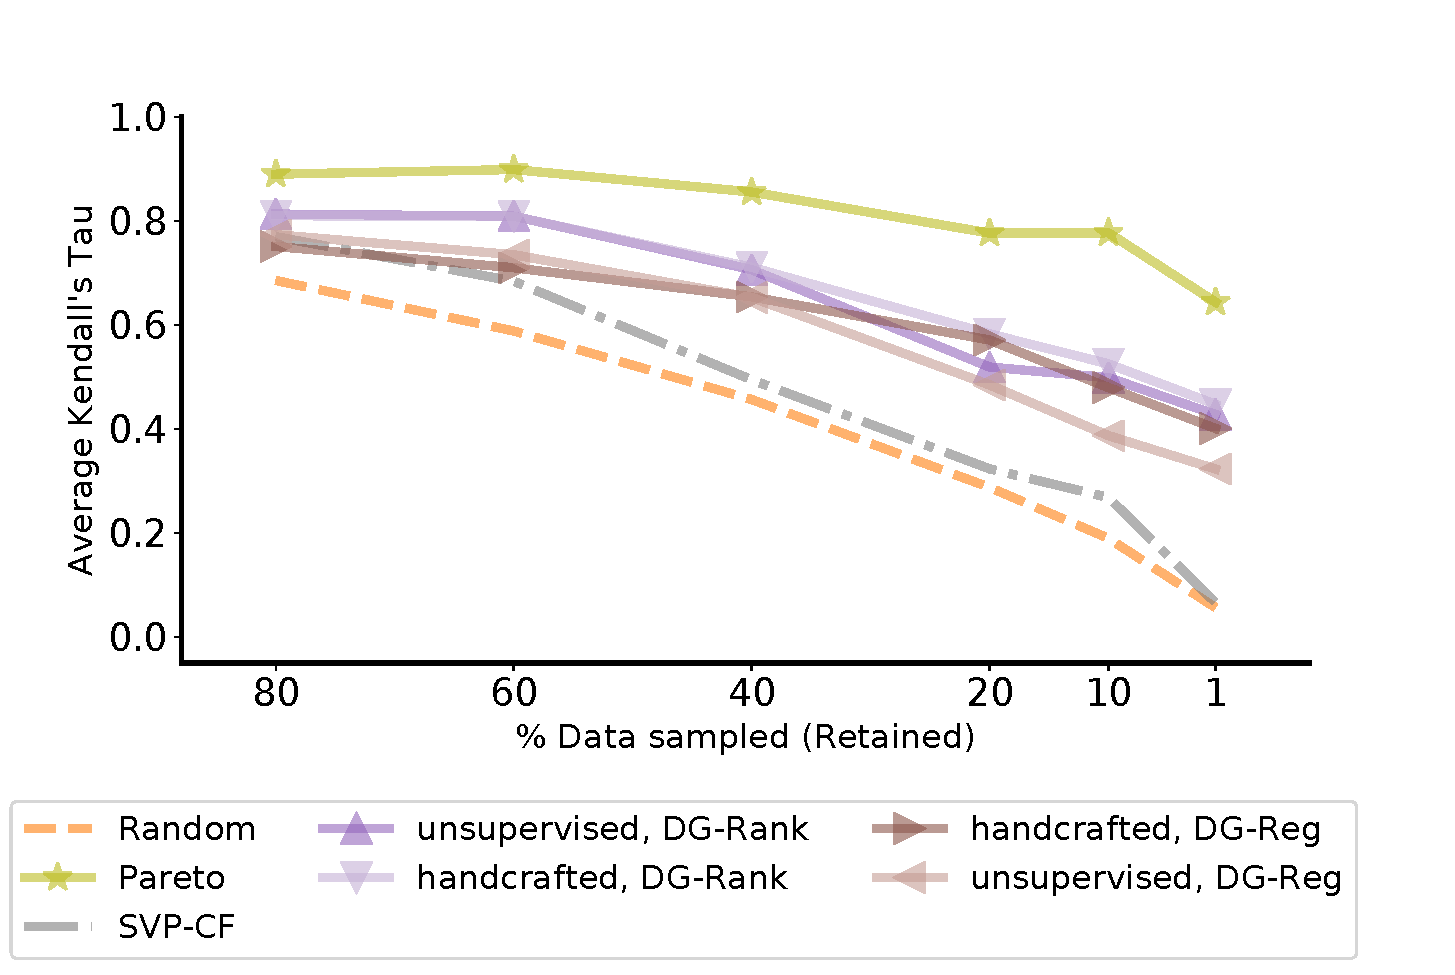
\includegraphics[width=0.86\linewidth]{figures/oracle_tau_vs_sampling_percent.pdf}
    \vspace{-0.1cm}
    \caption{Comparison of the average Kendall's Tau with \% data sampled for different sampling-selection strategies. A higher Tau indicates better retaining power of the ranking of different recommendation algorithms.}
    \label{percent_sampling_vs_tau_oracle}
\end{minipage}
\end{figure*} 

\subsection{Experiments}
\paragraph{Setup.} 
% We re-use the datasets, CF-scenarios, sampling strategies, and percentage sampling choices from \cref{main_exp}. To evaluate the competence of \oracle, we chose to perform the following train, validation, and test split: for each dataset and CF-scenario, we randomly split the metric and sampling percent $(m, p)$ join into $70/15/15\%$ proportions. Finally, during validation/testing, having fixed a dataset, CF-scenario, metric, and \% sampled data---we ask \oracle to predict the best sampler for this particular dataset. Given that there are only $16$ samplers in our study, we use the P$@1$ metric on the ranked list of samplers to evaluate \oracle.
We first create a train/validation/test split by randomly splitting all possible metrics and sampling $\%$ pairs $(m, p)$ into $70/15/15\%$ proportions. Subsequently for each dataset \dataset, CF-scenario $f$, and $(m, p)$ in the validation/test-set, we ask \oracle to rank all $16$ samplers (\cref{psi_results}) for $p\%$ sampling of $f-$type feedback for \dataset and use metric $m$ for evaluation by sorting $\hat{\tau}$ for each sampler, as defined in \cref{tau_hat}. To evaluate \oracle, we use the P$@1$ metric between the actual sampler ranking computed while computing $\Psi-$scores in \cref{main_exp}, and the one estimated by \oracle.
% Having already computed the true ranking of sampling strategies while computing $\Psi-$scores in \cref{main_exp}, we use the P$@1$ metric between the actual sampler ranking and the one estimated by sorting $\hat{\tau}$ for each sampler, as defined in \cref{tau_hat} to evaluate \oracle.

\subsubsection{How accurately can \oracle predict the best sampling scheme? \ \ } In \cref{oracle_results}, we compare all dataset representation choices $\mathcal{E}$, and multiple $\Phi$ architectures for the task of predicting the best sampling strategy. In addition to the regression and ranking architectures discussed in \cref{oracle_architecture}, we also compare with linear least-squares regression and XGBoost regression \cite{xgboost} as other choices of $\Phi$. In addition, we compare \oracle with simple baselines: (1) randomly choosing a sampling strategy; and (2) the best possible static sampler choosing strategy---always predict user sampling \emph{w/} Bias-only \samplerprop. First and foremost, irrespective of the $\mathcal{E}$ and $\Phi$ choices, \oracle outperforms both baselines. Next, both the handcrafted features and the unsupervised GCN features perform quite well in predicting the best sampling strategy, indicating that the graph characteristics are well correlated with the final performance of a sampling strategy. Finally, \oracle-regression and \oracle-ranking both perform better than alternative $\Phi-$choices, especially for the P$@1$ metric. 

% % \begin{table}[!ht]
    % \vspace{0.05cm}
    \begin{footnotesize} % normalsize, small, footnotesize
    \begin{center}
        \begin{tabular}{c c | c c c}
            \toprule
            $\mathcal{E}$ & $\Phi$ & \textbf{MSE} & \textbf{P@1} \\ \midrule
            
            \multicolumn{2}{c|}{Random} & 0.2336 & 25.2 \\ 
            \multicolumn{2}{c|}{User sampling \emph{w/} Bias-only \samplerprop} & -- & 30.6 \\ \midrule
            
            Handcrafted & Least squares regression & 0.1866 & 31.7 \\
            '' & XGBoost regression & 0.1163 & 43.9 \\
            '' & \oracle-regression & \underline{0.1008} & 51.2 \\ 
            '' & \oracle-ranking    & -- & 51.2 \\ \midrule
            
            Unsupervised GCN & Least squares regression & 0.1838 & 39.1 \\
            '' & XGBoost regression & 0.1231 & 43.9 \\
            '' & \oracle-regression & 0.1293 & 48.8 \\ 
            '' & \oracle-ranking    & -- & \underline{53.7} \\ \bottomrule
        \end{tabular}
    \end{center}
    \end{footnotesize}
    \vspace{0.5cm}
    \caption{Results for predicting the best sampling scheme for a particular dataset over a germane metric. The MSE-value next to randomly choosing the sampling scheme represents the variance of the test-set. Best values are \underline{underlined}.}
    \label{oracle_results}
    \vspace{-6mm} %Put here to reduce too much white space after your table
% \end{table}
% \begin{figure}[ht!] 
%     \centering
%     \vspace{-0.12cm}
%     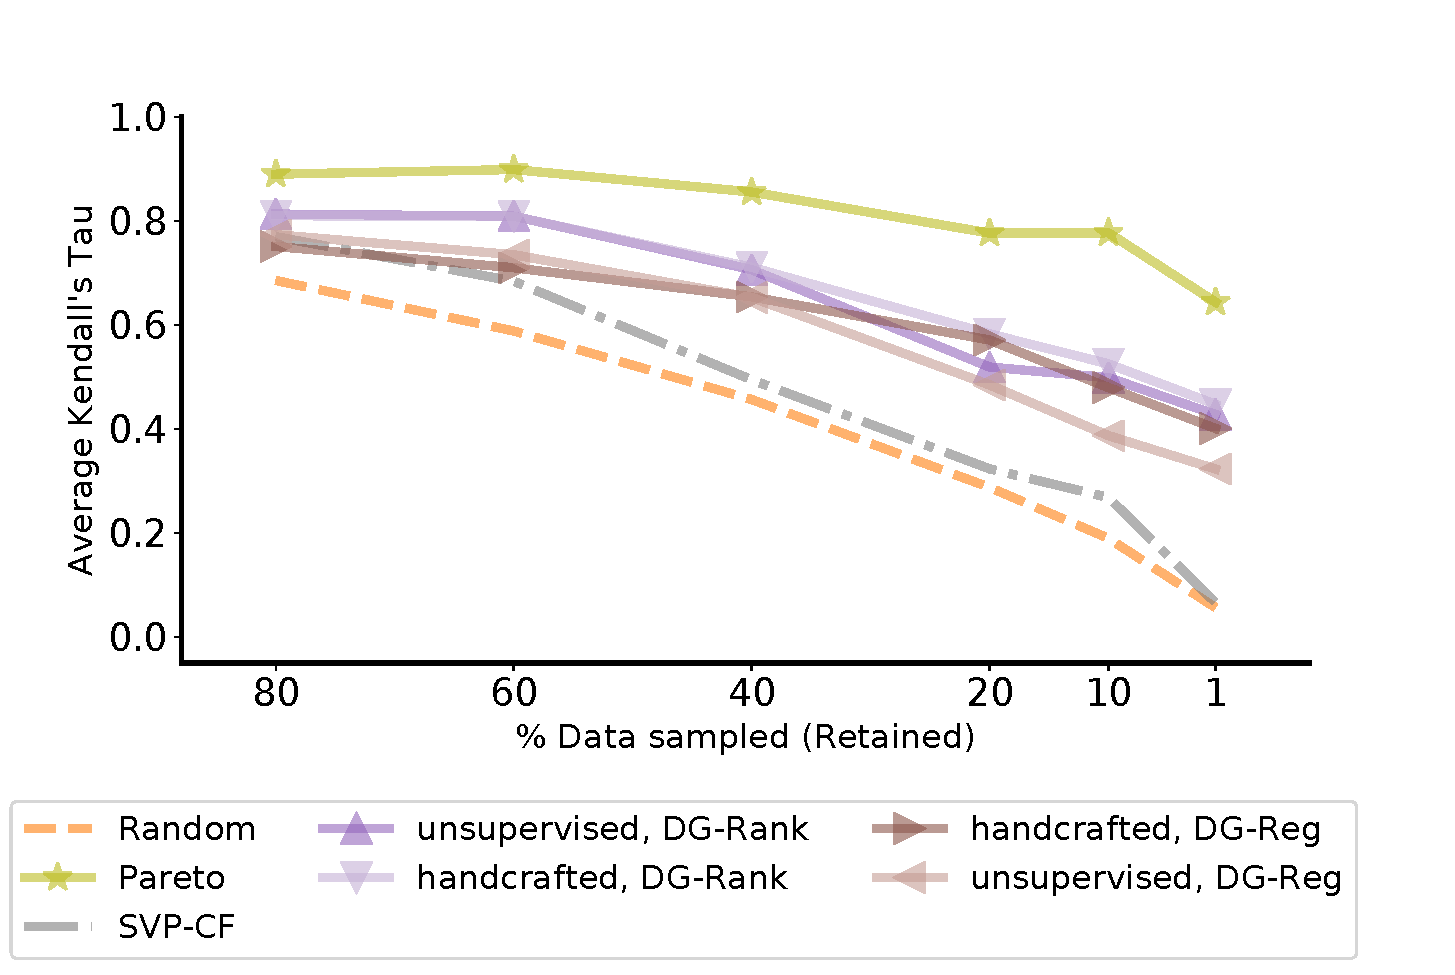
\includegraphics[width=\linewidth]{figures/oracle_tau_vs_sampling_percent.pdf}
%     \vspace{-0.5cm}
%     \caption{Comparison of the average Kendall's Tau with \% data sampled for different sampling-selection strategies. A higher Tau indicates better retaining power of the ranking of different recommendation algorithms.}
%     \label{percent_sampling_vs_tau_oracle}
% \end{figure} 

\subsubsection{Can we use \oracle to sample more data without compromising performance? \ \ } In \cref{percent_sampling_vs_tau_oracle}, we compare the impact of \oracle in sampling more data by dynamically choosing an appropriate sampler for a given dataset, metric, and $\%$ data to sample. 
% As a real-world benchmark for performance of \oracle, 
More specifically,
we compare the percentage of data sampled with the Kendall's Tau averaged over all datasets, CF-scenarios, and relevant metrics for different sampling strategy selection approaches. We compare \oracle with: (1) randomly picking a sampling strategy averaged over $100$ runs; and (2) the Pareto frontier as a skyline which always selects the best sampling strategy for any CF-dataset. As we observe from \cref{percent_sampling_vs_tau_oracle}, \oracle is better than predicting a sampling scheme at random, and 
% pushes the average Kendall's Tau
is
much closer to the Pareto frontier. Next, pairwise ranking approaches are marginally better than regression approaches 
% for both the handcrafted and unsupervised-GCN data features.
irrespective of $\mathcal{E}$. Finally, \oracle can appraise the best-performing recommendation algorithm with a suitable amount of confidence using only $10\%$ of the original data. This is significantly more efficient compared to having to sample $50-60\%$ if we were to always sample using a fixed strategy.
\newcommand{\STAB}[1]{\begin{tabular}{@{}c@{}}#1\end{tabular}}
\begin{table*}%[!ht]
    \begin{footnotesize}
    \begin{center}
        \begin{tabular}{c c | c c c c c c | c}
            \toprule
            \multicolumn{2}{c|}{\multirow{4}{*}{\textbf{Sampling strategy}}} & \multicolumn{6}{c|}{\emph{Datasets}} & \\
            & & \multicolumn{6}{c|}{} & \\
            & & \begin{tabular}{@{}c@{}}\textbf{Amazon}\\\textbf{Magazine}\end{tabular} & \textbf{ML-100k} & \begin{tabular}{@{}c@{}}\textbf{Amazon}\\\textbf{Luxury}\end{tabular} & \begin{tabular}{@{}c@{}}\textbf{Amazon}\\\textbf{Video-games}\end{tabular} & \textbf{BeerAdvocate} & \begin{tabular}{@{}c@{}}\textbf{Goodreads}\\\textbf{Comics}\end{tabular} & \textbf{\emph{Average}} \\
            \midrule
            
            \multirow{8}{*}{\STAB{\rotatebox[origin=c]{90}{\begin{tabular}{@{}c@{}}Interaction sampling\\\end{tabular}}}} & Random & 0.428     &  0.551     &  0.409     &  0.047     &  0.455     &  0.552     &  0.407 \\[0.6mm]
            & Stratified & 0.27      &  0.499     &  0.291     &  -0.01     &  0.468     &  0.538     &  0.343 \\[0.6mm]
            & Temporal & 0.289     &  0.569     &  0.416     &  -0.02     &  \underline{0.539}     &  0.634     &  0.405 \\[0.6mm]
            & \sampler \emph{w/} MF & 0.418     &  0.674     &  0.398     &  0.326     &  0.425     &  \underline{0.662}     &  \underline{0.484} \\[0.6mm]
            & \sampler \emph{w/} Bias-only & 0.38      &  0.684     &  \underline{0.431}     &  \underline{0.348}     &  0.365     &  0.6       &  0.468 \\[0.6mm]
            & \samplerprop \emph{w/} MF & 0.381     &  0.617     &  0.313     &  0.305     &  0.356     &  0.608     &  0.43 \\[0.6mm]
            & \samplerprop \emph{w/} Bias-only & 0.408     &  0.617     &  0.351     &  0.316     &  0.437     &  0.617     &  0.458 \\[0.6mm]
            \midrule
            \multirow{7}{*}{\STAB{\rotatebox[origin=c]{90}{\begin{tabular}{@{}c@{}}User sampling\\\end{tabular}}}} & Random & 0.436     &  0.622     &  0.429     &  0.17      &  0.344     &  0.582     &  0.431 \\[0.6mm]
            & Head & 0.369     &  0.403     &  0.315     &  0.11      &  -0.04     &  -0.02     &  0.19 \\[0.6mm]
            & \sampler \emph{w/} MF & 0.468     &  0.578     &  0.308     &  0.13      &  0.136     &  0.444     &  0.344 \\[0.6mm]
            & \sampler \emph{w/} Bias-only & 0.49      &  0.608     &  0.276     &  0.124     &  0.196     &  0.362     &  0.343 \\[0.6mm]
            & \samplerprop \emph{w/} MF & 0.438 &  0.683 &  0.307 &  0.098 &  0.458 &  0.592 &  0.429 \\[0.6mm]
            & \samplerprop \emph{w/} Bias-only & 0.434     &  \underline{0.751}     &  0.233     &  0.107     &  0.506     &  0.637     &  0.445 \\[0.6mm]
            \midrule
            \multirow{4}{*}{\STAB{\rotatebox[origin=c]{90}{\begin{tabular}{@{}c@{}}Graph\\\end{tabular}}}} & Centrality & 0.307     &  0.464     &  0.407     &  0.063     &  0.011     &  0.343     &  0.266 \\[0.6mm]
            & Random-walk & \underline{0.596}  &  0.5       &  0.395     &  0.306     &  0.137     &  0.442     &  0.396 \\[0.6mm]
            & Forest-fire & 0.564  &  0.493   &  0.415   &  0.265   &  0.099  &  0.454  &  0.382 \\[0.6mm]
            \bottomrule
        \end{tabular}
        % \begin{tabular}{c || c c c | c c | c c c}
        %     \toprule
        %     \multirow{3}{*}{Dataset} & \multicolumn{3}{c|}{Interaction sampling} & \multicolumn{2}{c|}{User sampling} & \multicolumn{3}{c}{Graph sampling} \\
        %     \multirow{2}{*}{} & \multicolumn{3}{c|}{} & \multicolumn{2}{c|}{} & \multicolumn{3}{c}{} \\
        %     & Random & Stratified & Temporal & Random & Head & Centrality & RW & FF \\ \midrule \midrule
            
        %     Amazon Magazine     & 0.428    & 0.27     & 0.289    & 0.436    & 0.369    & 0.307    & \underline{0.596} & 0.564 \\
        %     ML-100k             & 0.551    & 0.499    & 0.569    & 0.622    & 0.403    & 0.464    & 0.5      & 0.493 \\
        %     Amazon Luxury       & 0.409    & 0.291    & 0.416    & 0.429    & 0.315    & 0.407    & 0.395    & 0.415 \\
        %     Amazon Video-games  & 0.047    & -0.01    & -0.02    & 0.17     & 0.11     & 0.063    & 0.306    & 0.265 \\
        %     BeerAdvocate        & 0.455    & 0.468    & \underline{0.539}    & 0.344    & -0.04    & 0.011    & 0.137    & 0.099 \\
        %     Goodreads Comics    & 0.552    & 0.538    & 0.634    & 0.582    & -0.02    & 0.343    & 0.442    & 0.454 \\ \midrule
        %     Average             & 0.407    & 0.343    & 0.405    & 0.431    & 0.19     & 0.266    & 0.396    & 0.382 \\ \bottomrule 
        % \end{tabular}
        % \newline
        % \vspace*{0.5 cm}
        % \newline
        % \begin{tabular}{c || c c c c | c c c c}
        %     \toprule
        %     \multirow{4}{*}{Dataset} & \multicolumn{4}{c|}{Interaction sampling} & \multicolumn{4}{c}{User sampling} \\
        %     \multirow{2}{*}{} & \multicolumn{4}{c|}{} & \multicolumn{4}{c}{} \\
        %     & SVP-CF & SVP-CF-Prop & SVP-CF & SVP-CF-Prop & SVP-CF & SVP-CF-Prop & SVP-CF & SVP-CF-Prop \\
        %     & Bias-only & Bias-only & MF & MF & Bias-only & Bias-only & MF & MF \\ \midrule \midrule
            
        %     Amazon Magazine     & 0.38     & 0.408    & 0.418    & 0.381    & 0.49     & 0.434    & 0.468    & 0.438 \\
        %     ML-100k             & 0.684    & 0.617    & 0.674    & 0.617    & 0.608    & \underline{0.751}    & 0.578    & 0.683 \\
        %     Amazon Luxury       & \underline{0.431}    & 0.351    & 0.398    & 0.313    & 0.276    & 0.233    & 0.308    & 0.307 \\
        %     Amazon Video-games  & \underline{0.348}    & 0.316    & 0.326    & 0.305    & 0.124    & 0.107    & 0.13     & 0.098 \\
        %     BeerAdvocate        & 0.365    & 0.437    & 0.425    & 0.356    & 0.196    & 0.506    & 0.136    & 0.458 \\
        %     Goodreads Comics    & 0.6      & 0.617    & \underline{0.662}    & 0.608    & 0.362    & 0.637    & 0.444    & 0.592 \\ \midrule 
        %     Average             & 0.468    & 0.458    & \underline{0.484}    & 0.43     & 0.343    & 0.445    & 0.344    & 0.429 \\ \bottomrule
        % \end{tabular}
    \end{center}
    \end{footnotesize}
    \bigskip
    \caption{$\Psi$-values for all datasets and sampling strategies. Higher $\Psi$ is better. The best $\Psi$ for every dataset is \underline{underlined}. The $\Psi$-values for each sampling scheme \emph{averaged over all datasets} is appended to the right.}
    \label{psi_results}
    \vspace{-6mm} %Put here to reduce too much white space after your table
\end{table*}
%% This is file `sample-sigconf.tex',
\documentclass[sigconf]{acmart}

%%
%% \BibTeX command to typeset BibTeX logo in the docs
\AtBeginDocument{%
  \providecommand\BibTeX{{%
    \normalfont B\kern-0.5em{\scshape i\kern-0.25em b}\kern-0.8em\TeX}}}

%% Rights management information.  This information is sent to you
%% when you complete the rights form.  These commands have SAMPLE
%% values in them; it is your responsibility as an author to replace
%% the commands and values with those provided to you when you
%% complete the rights form.
\copyrightyear{2022}
\acmYear{2022}
\setcopyright{rightsretained}
\acmConference[WSDM '22]{Proceedings of the Fifteenth ACM
International Conference on Web Search and Data Mining}{February
21--25, 2022}{Tempe, AZ, USA}
\acmBooktitle{Proceedings of the Fifteenth ACM International Conference
on Web Search and Data Mining (WSDM '22), February 21--25, 2022,
Tempe, AZ, USA}
\acmDOI{10.1145/3488560.3498439}
\acmISBN{978-1-4503-9132-0/22/02}
%%
%% Submission ID.
%% Use this when submitting an article to a sponsored event. You'll
%% receive a unique submission ID from the organizers
%% of the event, and this ID should be used as the parameter to this command.
%%\acmSubmissionID{123-A56-BU3}

%%
%% The majority of ACM publications use numbered citations and
%% references.  The command \citestyle{authoryear} switches to the
%% "author year" style.
%%
%% If you are preparing content for an event
%% sponsored by ACM SIGGRAPH, you must use the "author year" style of
%% citations and references.
%% Uncommenting
%% the next command will enable that style.
%%\citestyle{acmauthoryear}

\usepackage{titlesec}
\usepackage{caption}
% \usepackage{subfigure}
\usepackage{subcaption}
\usepackage{booktabs}
\usepackage{multirow}
\usepackage{multicol}
\usepackage{xspace}
\usepackage{dsfont}
\usepackage{bbm}
\usepackage{bm}
\usepackage{pifont}
\usepackage{amsmath}
\usepackage{amsthm}
\usepackage{mathtools}
\usepackage{stackengine,scalerel}
% \usepackage{amssymb}
% \usepackage{float}
\usepackage{enumitem}
\usepackage{wrapfig}
\usepackage{caption}
\usepackage{cancel}
\setlist{leftmargin=5mm}

\usepackage{hyperref}
% \usepackage{cleveref}
\usepackage[capitalise, noabbrev]{cleveref}
% \usepackage[noabbrev]{cleveref}

\titleformat{\paragraph}[runin]{\bfseries\itshape}{\theparagraph}{1em}{}
\titlespacing*{\paragraph}{0pt}{3.25ex plus 1ex minus .2ex}{1em}

% Custom definitions
% \makeatletter \renewcommand\paragraph{\@startsection{paragraph}{4}{\z@} {2mm \@plus1ex \@minus.2ex} {-0.7em} {\normalfont\normalsize\bfseries}} \makeatother
\makeatletter \renewcommand\paragraph{\@startsection{paragraph}{4}{\z@} {2mm \@plus1ex \@minus.2ex} {-0.7em} {\normalfont\normalsize\itshape}} \makeatother

\newcommand{\listheader}[1]{\item \emph{#1} }

\newcommand\overstar[1]{\ThisStyle{\ensurestackMath{%
  \setbox0=\hbox{$\SavedStyle#1$}%
  \stackengine{0pt}{\copy0}{\kern.2\ht0\smash{\SavedStyle*}}{O}{c}{F}{T}{S}}}}

\newtheorem{theorem}{Theorem}[section]
\newtheorem{lemma}[theorem]{Lemma}
\newtheorem{proposition}[theorem]{Proposition}

\newcommand{\bs}[1]{\ensuremath{\bm{\mathit{#1}}}}

\newcommand{\ns}[1]{\textcolor{blue}{[Noveen: #1]}}
\newcommand{\jm}[1]{\textcolor{purple}{[Julian: #1]}}
\newcommand{\ie}[0]{\emph{i.e.}\xspace}
\newcommand{\etc}[0]{\emph{etc.}\xspace}
\newcommand{\eg}[0]{\emph{e.g.}\xspace}
\newcommand{\vs}[0]{\emph{vs.}\xspace}
\newcommand{\wrt}[0]{\emph{w.r.t.}\xspace}

\newcommand{\dataset}[0]{$\mathcal{D}$\xspace}
\newcommand{\sampled}[0]{$\mathcal{D}'$\xspace}
\newcommand{\argmin}[1]{\underset{#1}{\operatorname{arg}\,\operatorname{min}}\;}

\newcommand{\oracle}{\textsc{Data-genie}\xspace}
\newcommand{\sampler}{\textsc{SVP-CF}\xspace}
\newcommand{\samplerprop}{\textsc{SVP-CF-Prop}\xspace}

\newcommand{\EE}{\operatornamewithlimits{\mathbb{E}}} % Expectation

\allowdisplaybreaks % To break theorems into multiple pages

%%
%% end of the preamble, start of the body of the document source.
\settopmatter{printacmref=true}
\begin{document}
\fancyhead{}

%%
%% The "title" command has an optional parameter,
%% allowing the author to define a "short title" to be used in page headers.
\title{On Sampling Collaborative Filtering Datasets}

%%
%% The "author" command and its associated commands are used to define
%% the authors and their affiliations.
%% Of note is the shared affiliation of the first two authors, and the
%% "authornote" and "authornotemark" commands
%% used to denote shared contribution to the research.
\author{Noveen Sachdeva}
% \authornote{Both authors contributed equally to this research.}
\email{nosachde@ucsd.edu}
% \authornotemark[1] 
\affiliation{%
  \institution{University of California, San Diego}
  % \streetaddress{}
  \city{La Jolla, CA}
%   \state{CA, USA}
  \country{USA}
  \postcode{92122}
}

\author{Carole-Jean Wu}
\email{carolejeanwu@fb.com}
\affiliation{%
  \institution{Facebook AI Research}
  % \streetaddress{}
  \city{Cambridge, MA}
%   \state{CA, USA}
  \country{USA}
}

\author{Julian McAuley}
\email{jmcauley@ucsd.edu}
\affiliation{%
  \institution{University of California, San Diego}
  % \streetaddress{}
  \city{La Jolla, CA}
%   \state{CA, USA}
  \country{USA}
  \postcode{92122}
}

%%
%% By default, the full list of authors will be used in the page
%% headers. Often, this list is too long, and will overlap
%% other information printed in the page headers. This command allows
%% the author to define a more concise list
%% of authors' names for this purpose.
\renewcommand{\shortauthors}{Sachdeva, Wu, and McAuley}

%%
%% The abstract is a short summary of the work to be presented in the
%% article.
\begin{abstract}
  	
\begin{abstract}

Continuous Integration (CI) is a software development practice that builds and tests software frequently (e.g., at every push). One main motivator to adopt CI is the potential to deliver software functionalities more quickly than not using CI. However, there is little empirical evidence to support that CI helps projects deliver software functionalities more quickly. Through the analysis of 162,653 pull requests (PRs) of 87 GitHub projects, we empirically study whether adopting a CI service (\textsc{TravisCI}) can quicken the time to deliver merged PRs. 
We complement our quantitative study by analyzing 450 survey responses from participants of 73 software projects.
Our results reveal that adopting a CI service may not necessarily quicken the delivery of merge PRs. Instead, the pivotal benefit of a CI service is to improve the decision making on PR submissions, without compromising the quality or overloading the project's reviewers and maintainers. The automation provided by CI and the boost in developers' confidence are key advantages of adopting a CI service. Furthermore, open-source projects planning to attract and retain developers should consider the use of a CI service in their project, since CI is perceived to lower the contribution barrier while making contributors feel more confident and engaged in the project.
		
\keywords{Continuous Integration \and Pull Request \and Delivery Time \and Code Review}
 
\end{abstract}

\end{abstract}

%%
%% The code below is generated by the tool at http://dl.acm.org/ccs.cfm.
%% Please copy and paste the code instead of the example below.
%%

\begin{CCSXML}
<ccs2012>
<concept>
<concept_id>10002951.10003317.10003347.10003350</concept_id>
<concept_desc>Information systems~Recommender systems</concept_desc>
<concept_significance>500</concept_significance>
</concept>
<concept>
<concept_id>10010147.10010257.10010321.10010336</concept_id>
<concept_desc>Computing methodologies~Feature selection</concept_desc>
<concept_significance>300</concept_significance>
</concept>
</ccs2012>
\end{CCSXML}

\ccsdesc[500]{Information systems~Recommender systems}
\ccsdesc[300]{Computing methodologies~Feature selection}

%%
%% Keywords. The author(s) should pick words that accurately describe
%% the work being presented. Separate the keywords with commas.
\keywords{Sampling; Coreset Mining; Benchmarking; Large-scale Learning}

%% A "teaser" image appears between the author and affiliation
%% information and the body of the document, and typically spans the
%% page.

%%
%% This command processes the author and affiliation and title
%% information and builds the first part of the formatted document.
\maketitle

\section{Introduction} \section{Introduction}
\label{sec:introduction}
Before the early 1960s, it was believed that $CP$ is a good symmetry of nature. As Landau pointed out, that would make it impossible for particles to have electric dipole moments (EDMs) along their spin axis \cite{landau1957conservation}. The detection of such an EDM would thus provide clear evidence of $CP$-violation (CPV).  \blfootnote{*Present address: JILA, National Institute of Standards and Technology and University of
Colorado, and Department of Physics, Boulder, Colorado 80309, USA}

While most processes preserve $CP$, certain weak interactions violate it as observed in $K$-, $B$-, and $D$-meson decays \cite{christenson1964evidence, PDG18}. The flavor-changing part of the Standard Model (SM) quark sector includes a CPV phase in the CKM quark-mixing matrix \cite{peccei1995}. This so-called Kobayashi-Maskawa mechanism introduces the third quark generation to explain the CPV \cite{kobayashi1973cp}. The CKM phase has been the only source of observed CPV so far~\cite{PDG18}.

A major motivation for CPV searches comes from the baryon asymmetry of the universe (BAU). Compared to the current baryon density $n_{\text{B}}$, the antibaryon density $n_{\overline{\text{B}}}$ is very small; the reported upper bounds for the antimatter-to-matter number ratio range from $10^{-15}$ to $10^{-6}$ \cite{canetti2012matter}. To date, no mechanism has been experimentally verified that can explain the BAU. In a 1967 paper, Sakharov argued that CPV is necessary to explain the BAU \cite{sakharov1991violation} if the initial conditions of the universe were $C$-symmetric. The existing CPV in the CKM matrix is not enough to explain the extent of the BAU \cite{pospelov2005electric}. Thus new sources of CPV are required to explain the BAU.

No flavor-neutral CPV signal has been observed yet. However, many mechanisms can lead to such phenomena. For example, the QCD Lagrangian can, in principle, include an effective CPV term, proportional to the parameter $\bar{\theta}$~\cite{pospelov1999theta}:
\begin{equation}
	\mathcal{L} = \bar{\theta}\frac{g^2}{32\pi^2}G^a_{\mu\nu}\widetilde{G}^a_{\mu\nu},
\end{equation}
where $G^a$ is the gluon field tensor, $g$ is the strong coupling constant, and $\bar{\theta}$ is dimensionless. Experimental limits from experiments searching for CPV in neutral $^{199}$Hg atoms \cite{graner2016reduced} and ultracold neutrons \cite{baker2006improved, abel2020measurement} suggests that the strength of this term relative to the usual strong interaction is $\left|\bar{\theta}\right|<9\cdot10^{-11}$. The unexplained smallness of $\bar{\theta}$ is known as the strong $CP$ problem. One proposed solution to the strong $CP$ problem is the so called Peccei-Quinn mechanism, with an accompanying elementary scalar particle: the axion \cite{PhysRevLett.38.1440}. The axion would naturally lead to $\bar{\theta}\approx 0$, and is an attractive candidate for dark matter~\cite{PRESKILL1983127,PhysRevLett.50.925,PhysRevLett.124.101303}. (A review of experimental searches for the axion is given in \cite{graham2015experimental}.)

New hadronic $CP$-violating interactions from the QCD sector, or from physics beyond the SM, can lead to an effective charge asymmetry along the spin of a particle. Such charge asymmetries include EDMs and, for finite size particles such as nuclei, Schiff moments \cite{schiff1963measurability}. In the Standard Model, EDMs and nuclear Schiff moments (NSMs) are induced by the CKM phase, but are strongly suppressed: an EDM cannot appear below the three-loop level for quarks, or four-loop for leptons \cite{pospelov1991electric}. The CKM phase can produce a proton or neutron EDM no larger than $10^{-32}\,e\,$cm. Proposed extensions to the SM carry new CPV phases, which may manifest as EDMs or NSMs larger than expected based on the Standard Model. The search for an EDM or NSM thus constitutes a nearly background-free signal for new physics. In fact, the background expected from the Standard Model would only become apparent when probing effects beyond the energy scale of $\sim\!10^{5}\,$TeV \cite{pospelov2005electric}.

At present, searches for EDMs and related phenomena give the most sensitive constraints on flavor-neutral CPV effects beyond the SM. However, these searches are subject to the following limitation. According to the Schiff theorem, the interaction energy of nonrelativistic point-charged electric dipoles, bound in a neutral system but subject to an arbitrary external electrostatic potential, has no term linear in the CPV charge distribution \cite{schiff1963measurability}. Physically, the system rearranges itself so as to screen the external field completely \cite{safronova2018search}. Thus, a $CP$-violating moment of a charged constituent in a bound system cannot be detected without some mechanism to bypass Schiff's theorem. Two such mechanisms are relativistic constituent motion and finite constituent size. 

A nucleus in an atom or molecule is nonrelativistic, but has an extended size. This finite size can lead to a residual electromagnetic moment, the Schiff moment $\vec S$, that gives rise to a $CP$-violating interaction. In heavy diamagnetic atoms and diatomic molecules such as TlF, this finite-size effect gives the dominant contribution to CPV signals. Since the nuclear spin $\vec{I}$ is the only preferred direction in a nucleus, $\vec S$ has to lie parallel to this axis, i.e., $\vec{S} = S\vec{I}/I$. This quantum Schiff moment has the symmetries of $\vec{I}$: it changes sign under time reversal ($T$) but not under parity ($P$). By contrast, the classical Schiff moment is a static charge distribution that is unchanged under $T$ but changes sign under $P$. Hence, a nonzero value of $S$ means that both $T$ and $P$ symmetries are violated.
On the assumption that $CPT$ is a good symmetry, a nonzero value of $\vec S$ thus is also a signature of CPV.

The Schiff moment corresponds to a charge displacement that is similar to an EDM in its asymmetric distribution along the spin axis. It is equivalent to a charge density on the nuclear surface proportional to $\cos{\theta}$, where $\theta$ is the angle from $\vec{I}$; this surface charge distribution produces a uniform electric field inside the nucleus \cite{GingesFlambaum2004}. The magnitude $S$ of the NSM scales with the atomic mass $A$ as $S\propto A^{2/3}$ \cite{khriplovich1997}.

The value of $S$ can be related to more fundamental $CP$-violating parameters, including CPV $\pi$ meson--nucleon interaction constants $\bar{g}_{0},\,\bar{g}_1,$ and $\bar{g}_2$; the $\bar{\theta}$ QCD parameter; quark chromo-EDMs $\widetilde{d}_\text{d}$ and $\widetilde{d}_\text{u}$; and the neutron and proton EDMs, $d_\text{n}$ and $d_\text{p}$.  For example, the NSM of the $^{205}\mathrm{Tl}$ nucleus\footnote{The $^{205}\mathrm{Tl}$ nucleus has closed neutron shells; hence its NSM has negligible contribution from $d_\text{n}$.}  can be written as \cite{PhysRevA.101.042504,PhysRevA.101.042501}:
\begin{equation} 
    \label{eq:schiff_contributions}
        \begin{split}
            S\left(^{205}\mathrm{Tl}\right) & \approx \left(0.13g\bar{g}_0 - 0.004g\bar{g}_1 - 0.27 g \bar{g}_2\right) \,e\,\mathrm{fm}^3; \\
            S\left(^{205}\mathrm{Tl}\right) & \approx 0.027 \bar{\theta}\ e\,\mathrm{fm}^3; \\
            S\left(^{205}\mathrm{Tl}\right) & \approx \left(12\widetilde{d}_\text{d}+9\widetilde{d}_\text{u}\right) e\,\mathrm{fm}^2; \\
            S\left(^{205}\mathrm{Tl}\right) & \approx 0.4\,d_\text{p} \,\mathrm{fm}^2.
    \end{split}
\end{equation}
If detected, a nonzero $S\left(^{205}\mathrm{Tl}\right)$ would provide evidence for a nonzero value of one or more of these fundamental CPV parameters.

Energy shifts associated with a NSM can be greatly enhanced in polar molecules, where there is another intrinsic direction in addition to the nuclear spin: the internuclear axis $\hat{\vec{n}}$. In TlF,  we define $\hat{\vec{n}}$ as pointing from F to Tl, associated with the internal molecular dipole moment and a corresponding strong intramolecular gradient of the electron density.  For nuclei inside a molecule, the NSM (and other $CP$-violating effects \cite{khriplovich1997}) interacts with this density gradient, giving rise to an effective CPV Hamiltonian of the form \cite{PhysRevA.101.042504}
\begin{equation}\label{eq:Hamiltonian_effective_interaction}
    \mathcal{H}_\text{CPV}= W_S S\,\frac{\vec{I}}{I} \cdot \hat{\vec{n}}.
\end{equation}
Here, $W_S$ is the proportionality constant between $S$ and the CPV contribution to the molecular energy, for a fully polarized molecule. Its value is determined by the properties of the electronic wavefunctions, which can be calculated from first principles \cite{PhysRevA.101.042504, doi:10.1002/qua.20418, PhysRevLett.88.073001, doi:10.1080/00268976.2020.1767814}. The magnitude of $W_S$ grows rapidly with atomic number $Z$ of the nucleus, as $W_S\propto Z^2$ \cite{khriplovich1991parity}.

Without an external electric field $\Evec$, the interaction of Eq.~\ref{eq:Hamiltonian_effective_interaction} fails to produce a first-order effect in any given energy eigenstate. This is because the rotation of the molecule averages $\hat{\vec n}$ to zero, and the expectation value $\langle\mathcal{H}_\text{CPV}\rangle$ vanishes \cite{cho1989tenfold, cho1991search}. However, when an external field is applied, the molecule becomes polarized and both
%which destroys the inversion symmetry; then
$\hat{\vec{n}}$ and $\mathcal{H}_\text{CPV}$  acquire non-zero expectation values, with $\langle\hat{\vec n}\rangle \parallel \Evec$. We define the degree of electrical polarization $\mathcal{P} \equiv \langle \hat{\vec{n}}\cdot\hat{\Evec} \rangle$, (where $\hat{\Evec} = \Evec/\Esca$), so that $-1\leq\mathcal{P}\leq1$. 
%Here $\hat{z}$ is defined to be the axis along which the external electric field is applied. 
Hence, energy shifts due to CPV are given by  $\langle\mathcal{H}_\text{CPV}\rangle = W_S S \mathcal{P} \hat{\Evec} \cdot \frac{\vec{I}}{I}$.

\begin{figure}
    \centering
    \def\svgwidth{0.5\textwidth}
    \input{figs/svg/edm_levels.pdf_tex}
% 	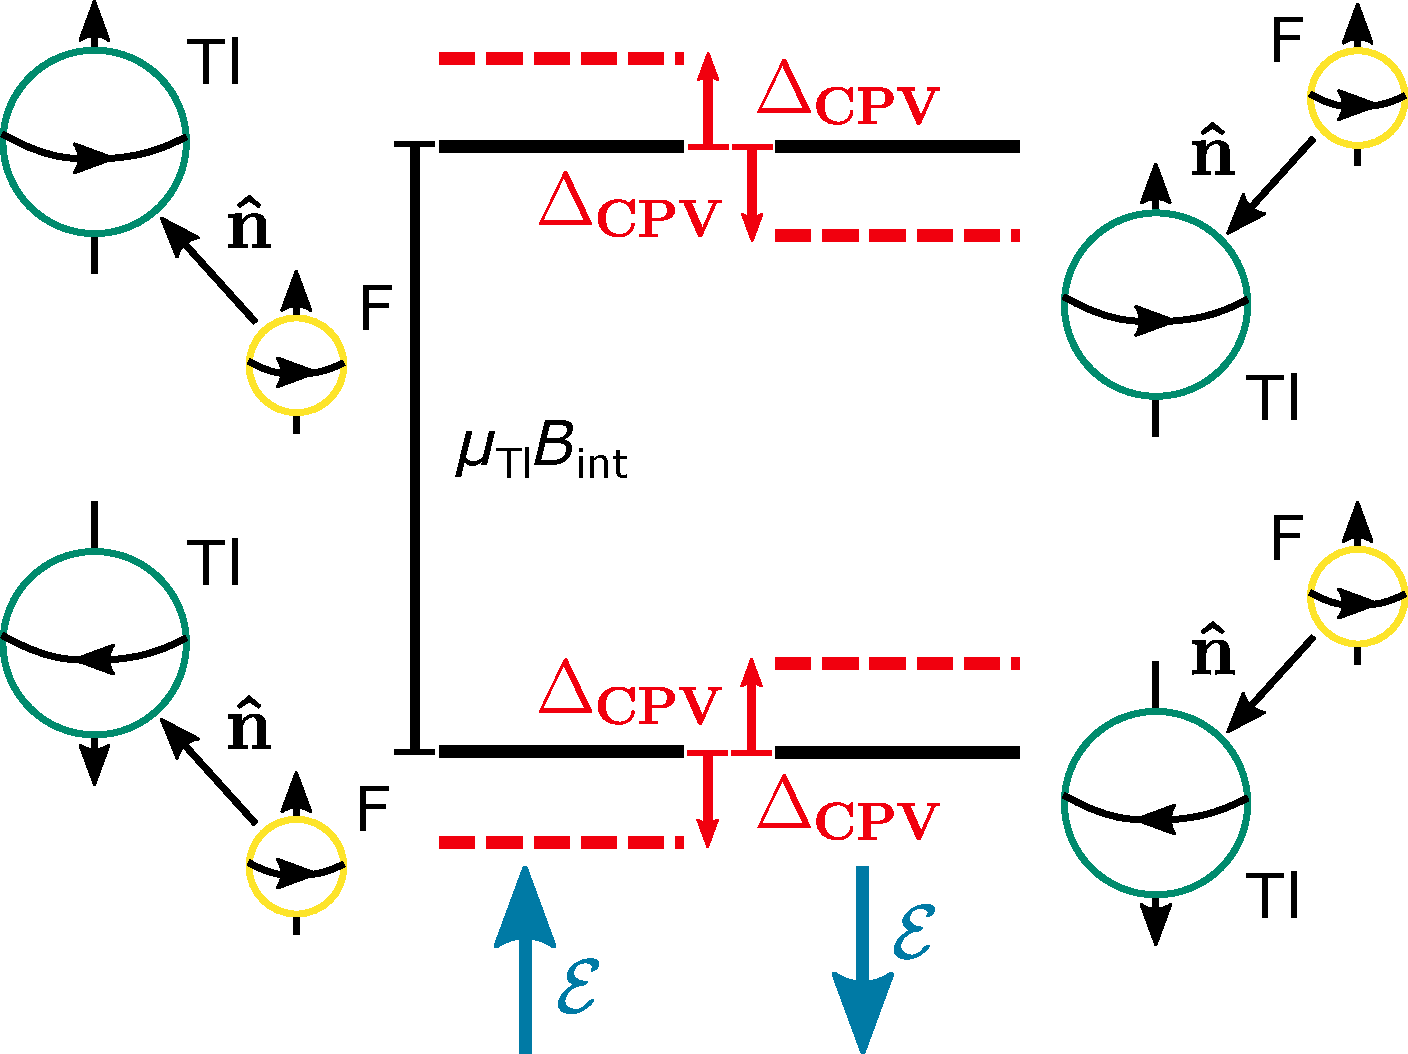
\includegraphics[width=0.48\textwidth,unit=1mm]{figs/svg/edm_levels_pdf_version.pdf}
	\caption{T-violating energy shift $\Delta_{\rm CPV} = W_SS\,\mathcal{P}$ as a result of a nonzero NSM $S$ given by the effective interaction $\mathcal{H}_\text{CPV}= W_S S\vec{I}\cdot \hat{\vec{n}}/I$ (Eq.~\ref{eq:Hamiltonian_effective_interaction}), shown for opposite orientations of the applied field $\Evec$. Here $\mu_1$ is the Tl magnetic moment and $B_1^\mathrm{int}$ is the effective internal magnetic field at the Tl nucleus due to the spin-rotation interaction.
	}
	\label{fig:edm_shift}
\end{figure}

Polar molecules can be polarized readily in laboratory-scale fields owing to their small rotational level separation ($\sim\!10^{-4}\eV$), giving them near-maximal energy shifts induced by a given Schiff moment. Thus, Sandars \cite{sandars1967measurability} suggested a molecular-beam resonance experiment could be used to probe the existence of the proton EDM, if the molecule has a heavy atom with an unpaired proton in the nucleus, such as $^{205}\mathrm{Tl}$. The value of $S$ is determined by measuring energy splittings between spin-up and -down states relative to $\left\langle \hat{\vec{n}}\right\rangle$ (which is parallel to the applied electric field $\bm{\mathcal{E}}$). This splitting will increase or decrease as $\bm{\mathcal{E}}$ (and hence $\left\langle \hat{\vec{n}}\right\rangle$) reverses, due to the interaction in Eq.~\ref{eq:Hamiltonian_effective_interaction}. The difference in level splittings is proportional to the electric polarization $\mathcal{P}$, the interaction strength $W_S$, and $S$ (Fig. \ref{fig:edm_shift}).

\CENTREX\ uses a cold beam of thallium fluoride (TlF) to measure nuclear $T$-violation due to the NSM of the $^{205}$Tl nucleus. It is a suitable system to look for $P$- and $T$-violating interactions for a number of reasons: a molecular beam of thallium fluoride can be readily obtained; many of the molecular states and transitions are known experimentally; the species is a polar diatomic molecule, enhancing the electron density gradient at the site of the nuclei (and hence $W_S$). As the thallium nucleus is heavy $\left(A=205,\,Z=81\right)$ and the NSM-induced energy shift scales $\propto A^{2/3}Z^2$, the observable effect of the Tl Schiff moment is correspondingly large \cite{sandars1967measurability, wilkening1984search}. Since the Tl nucleus contains an unpaired proton,
%the different linear combinations of underlying CPV parameters means
\CENTREX\ will be primarily sensitive to proton EDM effects, as opposed to other leading experiments which are more sensitive to the
%effects associated with neutron spin such as
neutron EDM \cite{graner2016reduced}. TlF is not very sensitive to the electron EDM due to its zero total electron spin \cite{kozlov1995parity}. 

The current best constraint on $T$-violating interactions associated with $S\left(^{205}\mathrm{Tl}\right)$ was found by Cho, Sangster and Hinds in 1991 \cite{cho1989tenfold, cho1991search}, who measured a NSM-induced frequency shift of $\Delta E = 2\Delta_{\rm CPV} = \left(1.4\pm 2.4\right)\times 10^{-4}$~Hz, consistent with zero.\footnote{Throughout, we express both frequencies and energies in linear frequency units (Hz), and all angular momentum operators are treated as dimensionless.} 
Using the effective interaction $\mathcal{H}_\text{CPV}$, the shift in the energy splitting between states with Tl spin up versus spin down, relative to the quantization axis, can be interpreted as
\begin{equation}
    \Delta E= 2 \Delta_{\rm CPV} = 2 W_S\,S\, \textrm{sgn}(\Esca) \,\mathcal{P},
    \label{eq:frequency_shift_due_to_NSM}
\end{equation}
where $W_S = 40539\,$a.u.,
polarization $\mathcal{P} = \langle\hat{\vec{n}} \cdot \hat{\Evec}\rangle = 0.547$, and the sign of $\Esca$ refers to the direction of $\Evec$ relative to a fixed quantizing axis $\hat{z}$.  This determines the Schiff moment \cite{PhysRevA.101.042501, PhysRevLett.88.073001}
\begin{equation}
    S\left(^{205}\mathrm{Tl}\right) = \left(3.6\pm 6.1\right)\times 10^{-11}\,e\,\mathrm{fm}^3.
\end{equation}
With Eq.~\ref{eq:schiff_contributions}, the following limits can be placed:
\begin{equation}
    \label{eq:prev_best_lims}
    \begin{split}
        \bar{\theta} & = \left(1.3 \pm 2.3\right)\ee{-9}, \\
        12\bar{d}_d+9\bar{d}_u & = \left(3.6\pm 6.1\right)\ee{-24}\,\mathrm{cm}, \\
        d_p          & = \left(0.9 \pm 1.5\right)\ee{-23}\,e\,\mathrm{cm},\\
        0.13g\bar{g}_0 - 0.004g\bar{g}_1-0.27g\bar{g}_2 & = \left(3.6 \pm 6.1\right)\ee{-11}.
    \end{split}
\end{equation}
\CENTREX\ aims to improve on these limits by using a cryogenic molecular beam source to achieve a cold beam with higher intensity and lower velocity spread compared to the jet source used in the previous work. Rotational cooling will be performed with optical and microwave pumping, collapsing much of the initial Boltzmann distribution into one state, greatly enhancing the number of molecules accessible for measurement. Finally, optical cycling will be used to assist state readout, resulting in near-unity detection efficiency. Fluorescence detection, compared to the hot-wire techniques used previously, allows for background-free detection if scattered light is well controlled.

\subsection{Thallium Fluoride}
\label{sec:tlf_theory}

\begin{figure}
	    % for axis breaks
    \usetikzlibrary{decorations.markings}
    \def\MarkLt{4pt}
    \def\MarkSep{2pt}
    \tikzset{
      TwoMarks/.style={
        postaction={decorate,
          decoration={
            markings,
            mark=at position #1 with
              {
                  \begin{scope}[xslant=0.2]
                  \draw[line width=\MarkSep,white,-] (0pt,-\MarkLt) -- (0pt,\MarkLt) ;
                  \draw[-] (-0.5*\MarkSep,-\MarkLt) -- (-0.5*\MarkSep,\MarkLt) ;
                  \draw[-] (0.5*\MarkSep,-\MarkLt) -- (0.5*\MarkSep,\MarkLt) ;
                  \end{scope}
              }
           }
        }
      },
      TwoMarks/.default={0.5},
    }

\begin{tikzpicture}[scale=5]

   % length of energy level diagram lines
   \def\len{.05}

   % x-position and length and x-offset of the y-axis labels
   \def\pos{-18}
   \def\lenmark{.025}
   \def\xoffset{.18}

   % x coordinates for m = -2, ... 2
   \def\xa{-4.5*\len}
   \def\xb{-2.5*\len}
   \def\xc{-0.5*\len}
   \def\xd{+1.5*\len}
   \def\xe{+3.5*\len}
   \def\xf{-6.5*\len}
   \def\xg{+5.5*\len}

   % y offset for J = 1, 2
   \def\yA{.6}
   \def\yB{\yA+.7}

   % axis
   \draw[->,TwoMarks=0.2,TwoMarks=0.6] (\xf-\len-\xoffset, -.1)
      -- (\xf-\len-\xoffset,\yB+.25) node[above, xshift = -20] {$E$ [kHz]};

   % brace position
   \def\bracePos{\xg+3*\len}

    
   % J=0 labels
   \draw [decorate,decoration={brace,amplitude=5pt,mirror,raise=4pt},yshift=0pt]
      (\bracePos,-.08) -- node (midJ0) {} (\bracePos,.08) node [black,midway,anchor=west,xshift=25] (nodeJ0) {$0$};
   \draw (\xf-\len-0.5*\lenmark-\xoffset, -.003325) node[anchor=east,below,xshift=\pos]
      {-3.325} -- (\xf-\len+0.5*\lenmark-\xoffset,-.003325) node[right,below,xshift=-\pos] {$1$};
   \draw (\xf-\len-0.5*\lenmark-\xoffset, .009975) node[anchor=east,above,xshift=\pos]
      {9.975} -- (\xf-\len+0.5*\lenmark-\xoffset,.009975) node[right,above,xshift=-\pos] {$0$};

   % J=0 lines
   \draw (\xc, -0.003325) -- (\xc+\len, -0.003325);
   \draw (\xb, -0.003325) -- (\xb+\len, -0.003325);
   \draw (\xd, -0.003325) -- (\xd+\len, -0.003325);
   \draw (\xc, 0.009975) -- (\xc+\len, 0.009975);

   % J=1 labels
   \draw [decorate,decoration={brace,amplitude=10pt,mirror,raise=4pt},yshift=0pt]
      (\bracePos,\yA-.2) -- node (midJ1) {} (\bracePos,\yA+.1) node [black,midway,anchor=west,xshift=25] (nodeJ1) {$1$};
   \draw (\xf-\len-0.5*\lenmark-\xoffset, \yA-.143745) node[anchor=east,below,xshift=\pos] {-143.745} --
      (\xf-\len+0.5*\lenmark-\xoffset,\yA-.143745) node[right,below,xshift=-\pos] {$0$};
   \draw (\xf-\len-0.5*\lenmark-\xoffset, \yA-.121506) node[anchor=east,above,xshift=\pos] {-121.506} --
      (\xf-\len+0.5*\lenmark-\xoffset,\yA-.121506) node[right,above,xshift=-\pos] {$1$};
   \draw (\xf-\len-0.5*\lenmark-\xoffset, \yA+.054446) node[anchor=east,below,xshift=\pos] {54.446} --
      (\xf-\len+0.5*\lenmark-\xoffset,\yA+.054446) node[right,below,xshift=-\pos] {$1$};
   \draw (\xf-\len-0.5*\lenmark-\xoffset, \yA+.068985) node[anchor=east,above,xshift=\pos] {68.985} --
      (\xf-\len+0.5*\lenmark-\xoffset,\yA+.068985) node[right,above,xshift=-\pos] {$2$};

   % J=1 lines
   \draw (\xc, \yA-.143745) -- (\xc+\len, \yA-.143745);
   \draw (\xc, \yA-.121506) -- (\xc+\len, \yA-.121506);
   \draw (\xb, \yA-.121506) -- (\xb+\len, \yA-.121506);
   \draw (\xd, \yA-.121506) -- (\xd+\len, \yA-.121506);
   \draw (\xc, \yA+.054446) -- (\xc+\len, \yA+.054446);
   \draw (\xb, \yA+.054446) -- (\xb+\len, \yA+.054446);
   \draw (\xd, \yA+.054446) -- (\xd+\len, \yA+.054446);
   \draw (\xc, \yA+.068985) -- (\xc+\len, \yA+.068985);
   \draw (\xb, \yA+.068985) -- (\xb+\len, \yA+.068985);
   \draw (\xd, \yA+.068985) -- (\xd+\len, \yA+.068985);
   \draw (\xa, \yA+.068985) -- (\xa+\len, \yA+.068985);
   \draw (\xe, \yA+.068985) -- (\xe+\len, \yA+.068985);

   % J=2 labels
   \draw [decorate,decoration={brace,amplitude=10pt,mirror,raise=4pt},yshift=0pt]
      (\bracePos,\yB-.27) -- node (midJ2) {} (\bracePos,\yB+.18) node [black,midway,anchor=west,xshift=25] (nodeJ2) {$2$};
   \draw (\xf-\len-0.5*\lenmark-\xoffset, \yB-.217455)
   node[anchor=east,left,yshift=-5] {-217.455}
      -- (\xf-\len+0.5*\lenmark-\xoffset,\yB-.217455) node[right,below,xshift=-\pos] {$1$};
   \draw (\xf-\len-0.5*\lenmark-\xoffset, \yB-.172936)
   node[anchor=east,left,yshift=5] {-172.936}
      -- (\xf-\len+0.5*\lenmark-\xoffset,\yB-.172936) node[right,above,xshift=-\pos] {$2$};
   \draw (\xf-\len-0.5*\lenmark-\xoffset, \yB+.105876)
   node[anchor=east,left,yshift=-5] {105.876}
      -- (\xf-\len+0.5*\lenmark-\xoffset,\yB+.105876) node[right,below,xshift=-\pos] {$2$};
   \draw (\xf-\len-0.5*\lenmark-\xoffset, \yB+.141095)
   node[anchor=east,left,yshift=5] {141.095}
      -- (\xf-\len+0.5*\lenmark-\xoffset,\yB+.141095) node[right,above,xshift=-\pos] (J2F3label) {$3$};

   % J=2 lines
   \draw (\xc, \yB-.217455) -- (\xc+\len, \yB-.217455);
   \draw (\xb, \yB-.217455) -- (\xb+\len, \yB-.217455);
   \draw (\xd, \yB-.217455) -- (\xd+\len, \yB-.217455);
   \draw (\xc, \yB-.172936) -- (\xc+\len, \yB-.172936);
   \draw (\xb, \yB-.172936) -- (\xb+\len, \yB-.172936);
   \draw (\xd, \yB-.172936) -- (\xd+\len, \yB-.172936);
   \draw (\xa, \yB-.172936) -- (\xa+\len, \yB-.172936);
   \draw (\xe, \yB-.172936) -- (\xe+\len, \yB-.172936);
   \draw (\xc, \yB+.105876) -- (\xc+\len, \yB+.105876);
   \draw (\xb, \yB+.105876) -- (\xb+\len, \yB+.105876);
   \draw (\xd, \yB+.105876) -- (\xd+\len, \yB+.105876);
   \draw (\xa, \yB+.105876) -- (\xa+\len, \yB+.105876);
   \draw (\xe, \yB+.105876) -- (\xe+\len, \yB+.105876);
   \draw (\xc, \yB+.141095) -- (\xc+\len, \yB+.141095);
   \draw (\xb, \yB+.141095) -- (\xb+\len, \yB+.141095);
   \draw (\xd, \yB+.141095) -- (\xd+\len, \yB+.141095);
   \draw (\xa, \yB+.141095) -- (\xa+\len, \yB+.141095);
   \draw (\xe, \yB+.141095) -- (\xe+\len, \yB+.141095);
   \draw (\xf, \yB+.141095) -- (\xf+\len, \yB+.141095);
   \draw (\xg, \yB+.141095) -- (\xg+\len, \yB+.141095);

   % microwave energies
   \draw[Latex-Latex] (nodeJ0) -- node[above,sloped] {13.3 GHz} (nodeJ1);
   \draw[Latex-Latex] (nodeJ1) -- node[above,sloped] {26.7 GHz} (nodeJ2);

   % approximate F1 labels
   \def\FposX{-5}
   \def\FposY{15}
   \def\FposYY{22}
   \node[xshift=\FposX] at (midJ0) {\nicefrac{1}{2}};
   \node[xshift=\FposX,yshift=-\FposY] at (midJ1) {\nicefrac{1}{2}};
   \node[xshift=\FposX, yshift=\FposY] at (midJ1) {\nicefrac{3}{2}};
   \node[xshift=\FposX,yshift=-\FposYY] at (midJ2) {\nicefrac{3}{2}};
   \node[xshift=\FposX, yshift=\FposYY] at (midJ2) {\nicefrac{5}{2}};
   \node[xshift=\FposX, yshift=47] at (midJ2) (F1label) {$F_1$};
    
   \node at (F1label -| nodeJ2) {$J$};
   \node at (F1label -| J2F3label) {$F$};

\end{tikzpicture}

	\caption{Hyperfine structure in the lowest three rotational levels in the TlF ground state $X^1\Sigma^+$, with no applied fields. Rotational energies $hBJ(J+1)$ should be added to
	%are subtracted from
	the hyperfine energy shifts indicated on the axis. Note the $(2F+1)$-fold degeneracy of each state with total angular momentum $F$, corresponding to the quantum numbers $m_F=-F,\dots,0,\dots,F$.}
	\label{fig:level_diagram}

\end{figure}

The TlF molecule is described by its electronic, vibrational and rotational motion, plus the states of the Tl and F nuclear spins. \CENTREX\ makes use of states both in the vibronic ground state, $X ^1\Sigma^+\left(\nu=0\right)$, and in an electronically excited state, $B ^3\Pi_1\left(\nu=0\right)$.  In both cases, we describe the angular momentum couplings in a Hund's case (a) basis. We typically write energy eigenstates in terms of the basis states $\ket{\eta,J,F_1,F,m_F}$. Here, $\eta$ represents the vibronic quantum numbers; $J$ is the total angular momentum excluding the nuclear spins, $\vec{F}_1 = \vec{J}+\vec{I}_\mathrm{1}$, with $I_\mathrm{1}=1/2$ for $^{205}$Tl; $\vec{F} = \vec{F}_1+\vec{I}_\mathrm{2}$ is the total angular momentum, with $I_\mathrm{2}=1/2$ for $^{19}$F; and $m_F$ is its projection along a quantization axis in the lab frame. Field-free eigenstates are close to these basis states in the ground $X ^1\Sigma^+$ state.  In the $B ^3\Pi_1$ state, strong hyperfine interactions significantly mix states with different $J$ and $F_1$ values. Hence, we describe these eigenstates with the modified notation $\ket{\eta',\widetilde{J}' ,\widetilde{F}_1^\prime,F',m_F'}$, where $\widetilde{J}'$ and $\widetilde{F}_1^\prime$ correspond to the largest component in their basis-state decomposition; the primes indicate that the ket refers to the excited state $B ^3\Pi_1$.

Molecules in the beam are assumed to be in the vibronic ground state, since the beam temperature is much lower than the energy scales associated with the electronic and vibrational excitations. However, even at cryogenic temperatures, there is a Boltzmann distribution over many rotational and nuclear spin states. The dominant term in the energy of rotational/spin levels in the $X ^1\Sigma^+$ state is due to rotation; the mean energy of states with quantum number $J$ is $E_\mathrm{rot}=BJ(J+1)$, where $B\approx 6.67\GHz \approx 0.3\kelvin\,\kB$, where $\kB$ the Boltzmann constant.\footnote{In Ramsey et al.\ \cite{wilkening1984search}, the symbol $B$ denotes the rotational constant in equilibrium position, i.e., there $B\equiv B_\text{e}$. However, the effective $v=0$ rotational constant, $B_0$, is more relevant to \CENTREX. To first order in the Dunham expansion \cite{huber2013molecular}, $B_0=B_\text{e}-\alpha_\text{e}/2$. With $B_\text{e}$ and $\alpha_\text{e}$ from the NIST database \cite{afeefy2011nist}, we find $B_0$. We define the symbol $B\equiv B_0$; its value is shown in Table~\ref{tab:hyperfine_hamiltonian}.}

Hyperfine interactions split sublevels with different $F$ values ($F=J-1,J,J, J+1$, except $F=0,1$ only for $J=0$) in each rotational state. Thus, each rotational level has $4(2J+1)$ magnetic sublevels. %including nuclear spins.
Including rotation, spin-rotation and spin-spin interactions, plus interactions with external electric $(\Evec)$ and magnetic $(\Bvec)$ fields, the system is described by the effective Hamiltonian \cite{wilkening1984search}
\small
$\mathcal{H}_\text{TlF} = \mathcal{H}_\text{rot}+\mathcal{H}_\text{sr}+\mathcal H_\text{ss} + \mathcal H_\text{S}+\mathcal H_\text{Z}$, 
\normalsize
where
\begin{equation} 
    \label{eq:hyperfine_hamiltonian}
    \begin{split}
        \mathcal H_\text{rot} & = B \vec{J}^2 \\
        \mathcal H_\text{sr}&=c_1(\vec I_1\cdot\vec J)+c_2(\vec I_2\cdot\vec J), \\
        \mathcal H_\text{ss}&=c_3 T^2(\vec C)\cdot T^2(\vec I_1, \vec I_2)+c_4(\vec I_1\cdot\vec I_2), \\
        \mathcal H_\text{S}&=-\vec\mu_e\cdot\vec \Evec,\\
        \mathcal H_\text{Z}&=-\frac{\mu_J}{J}(\vec J\cdot\vec \Bvec)-\frac{\mu_1}{I_1}(\vec I_1\cdot\vec \Bvec)-\frac{\mu_2}{I_2}(\vec I_2\cdot\vec \Bvec).
    \end{split}
\end{equation}
Here, the first term in the spin-spin interaction ($\mathcal H_\text{ss}$) contains the scalar product of two rank-2 tensors: one constructed from the modified spherical harmonics $\vec C$, and one from $\vec{I}_1$ and $\vec{I}_2$ \cite{brown2003rotational}. (The matrix elements diagonal in $J$ of this term are given in \cite{wilkening1984search}.)  The hyperfine parameters $c_1,c_2,c_3,c_4$, rotational constant $B$, magnetic moments $\mu_J,\mu_1,\mu_2$, and molecule-frame electric dipole moment $\mu_e$ are all known from previous measurements; their values are given in  Table~\ref{tab:hyperfine_hamiltonian}. A level diagram of low-lying states in the absence of applied fields is shown in Fig.~\ref{fig:level_diagram}.

\begin{table}
    \small
    \setlength\extrarowheight{3pt}
    \rowcolors{2}{white}{gray!25}
	\centering
	\caption{Constants describing rotational, hyperfine, Zeeman, and Stark interactions in the effective TlF ground-state  Hamiltonian (Eq.~\ref{eq:hyperfine_hamiltonian}). All values taken from Ramsey et al.\ \cite{wilkening1984search}, except for $B$ (see Sec. \ref{sec:tlf_theory}).}
	\label{tab:hyperfine_hamiltonian}
	\begin{tabular}{r@{\hspace{5pt}}c@{\hspace{5pt}}l@{\hspace{5pt}}l | r@{\hspace{5pt}}c@{\hspace{5pt}}l@{\hspace{5pt}}l}
    	\toprule
		$B$ & = &           $6.66733$ &     GHz &       $\mu_e$ & = & $4.2282(8)$ &     Debye \\
		$\mu_J$ & = &       $35(15)$ &      Hz/G &      $c_1$ & = & $126.03(12)$ &    kHz \\
		$\mu_1^{205}$ & = & $1.2405(3)$ &   kHz/G &     $c_2$ & = & $17.89(15)$ &     kHz\\
		$\mu_1^{203}$ & = &  $1.2285(3)$ &   kHz/G &     $c_3$ & = & $0.70(3)$ &       kHz \\
		$\mu_2$ & = &      $2.00363(4)$ &  kHz/G  &    $c_4$ & = & $-13.30(72)$ &    kHz \\
		\bottomrule
	\end{tabular}
\end{table}

%%%%%%%%%%%%%%%%%%%%%%%%%%%%%%%%%%%%%%%%%%%%%%55%%%%%%%%%%%%%%%
In \CENTREX, lasers are tuned to $X^1\Sigma^+(\nu=0)\rightarrow B^3\Pi_1\left(\nu=0\right)$ transitions in order to manipulate and read out ground state hyperfine and rotational sublevels. Details of the $B ^3\Pi_1$ state structure are given in \cite{norrgard2017hyperfine,PhysRevA.101.042506}.  Here, only a few main features of the $B$ state substructure are important.  First, the $B$ state hyperfine splittings are very large ($\gtrsim 100\MHz$) compared to the natural linewidth of the transition ($\gamma_B \approx 1.6\MHz$), which is in turn much larger than the ground-state hyperfine splittings ($c_j \lesssim 100\kHz$). This means that hyperfine structure is fully resolved in the excited state, and entirely unresolved in the ground state. Hence, optical transitions in TlF drive a large manifold of ground-state hyperfine levels (with a given value of $J$) to a single hyperfine state with (nominal) quantum numbers $\tilde{J},\tilde{F}_1$ and exact quantum number $F$. Another important feature of the $B$ state is that its matrix of Franck-Condon factors (FCFs) for decay to the $X$ state is extremely diagonal \cite{hunter2012prospects}, such that $\sim\! 99\%$ of the time, the $B(v=0)$ vibronic state decays back to the vibronic ground state $X(v=0)$.  This enables optical pumping and optical cycling with little loss.  However, the mixing of $J$ and $F_1$ by the strong $B$-state hyperfine interaction substantially modifies rotational selection rules in $B-X$ decays, and must be taken into account when describing optical excitation and emission in TlF.

\subsection{TlF in \texorpdfstring{$\Esca$}{E}-fields}
\label{sec:TlF_in_E_fields}

\begin{figure*}
	\centering
	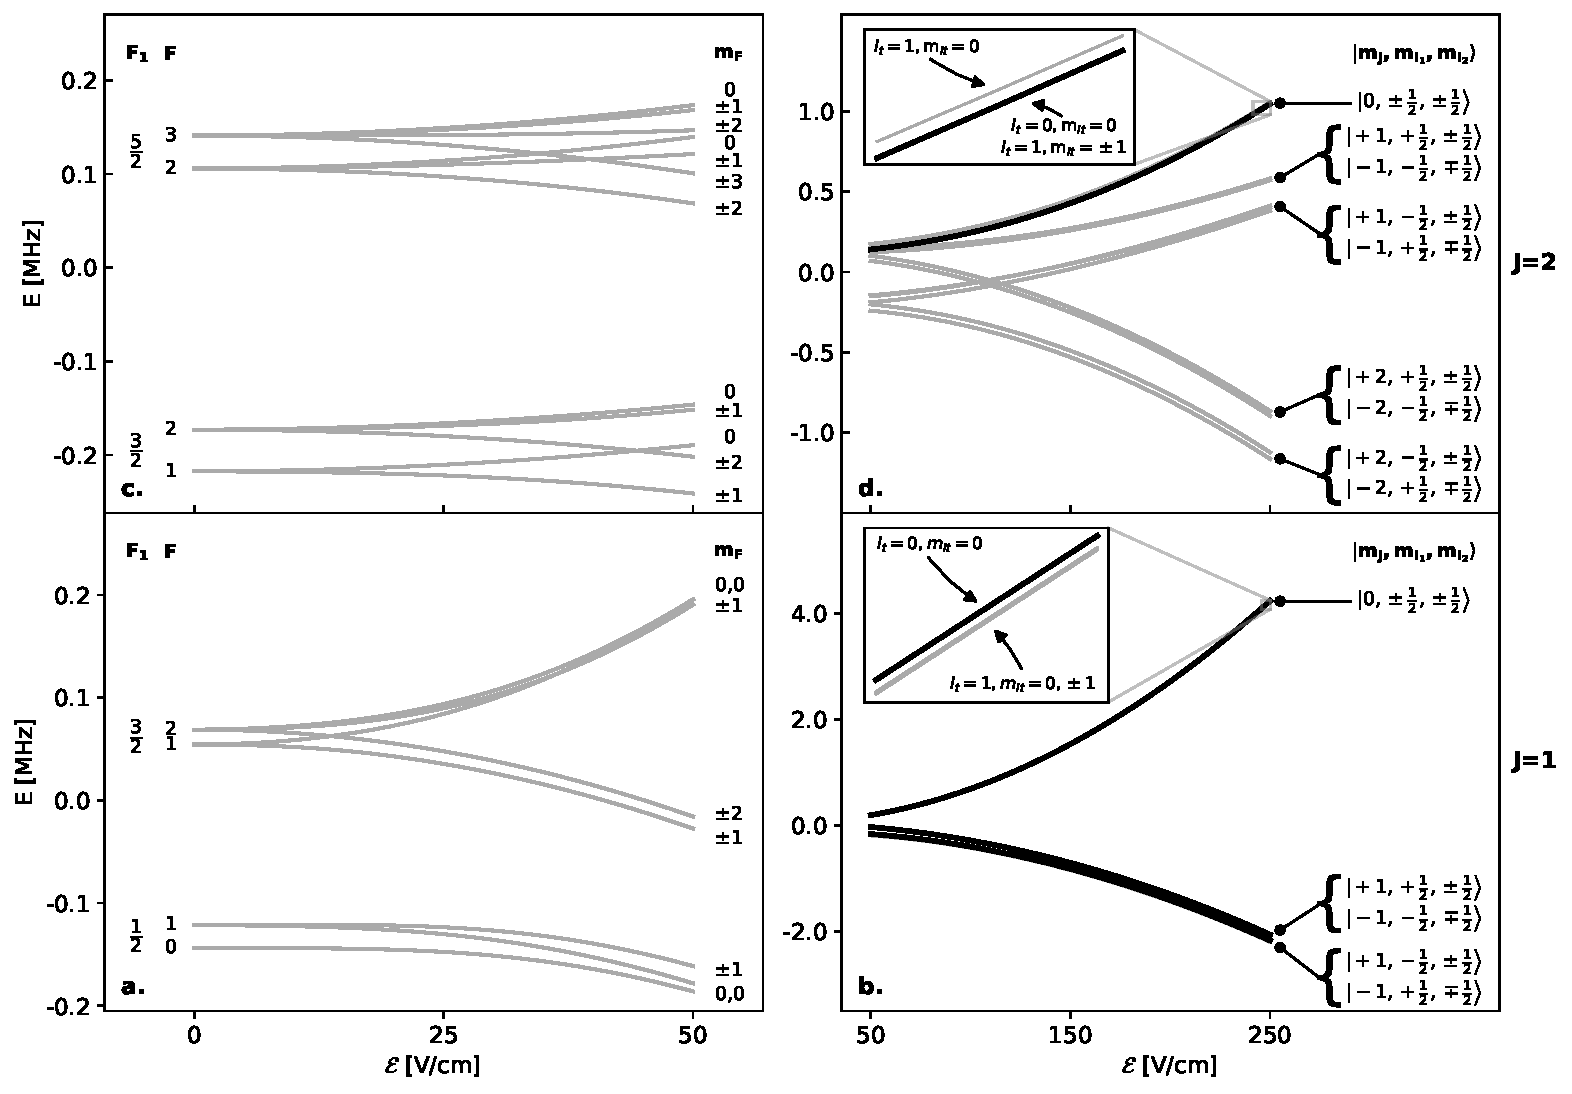
\includegraphics[width=\textwidth]{figs/matplotlib/low_to_mid_field.pdf}
	\caption{Overview of the energy eigenstates for changing $\Esca$-field magnitudes. The low-field regime, where $\Delta E_{\rm S} \ll E_{\rm hf}$, where energy eigenstates retain $J$, $F$, and $F_1$ as approximate quantum numbers is shown in \part{a} for $J=1$ and \part{c} for $J=2$. The mid-field regime, where $E_{\rm hf} \ll \Delta E_{\rm S} \ll E_{\rm rot}$, where both $J$ and $m_J$ are approximate quantum numbers is shown in \part{b} for $J=1$ and \part{d} for $J=2$. States used in \CENTREX\ are shown in bold.}
	\label{fig:low_to_mid_field}
\end{figure*}

\begin{figure}
	\centering
	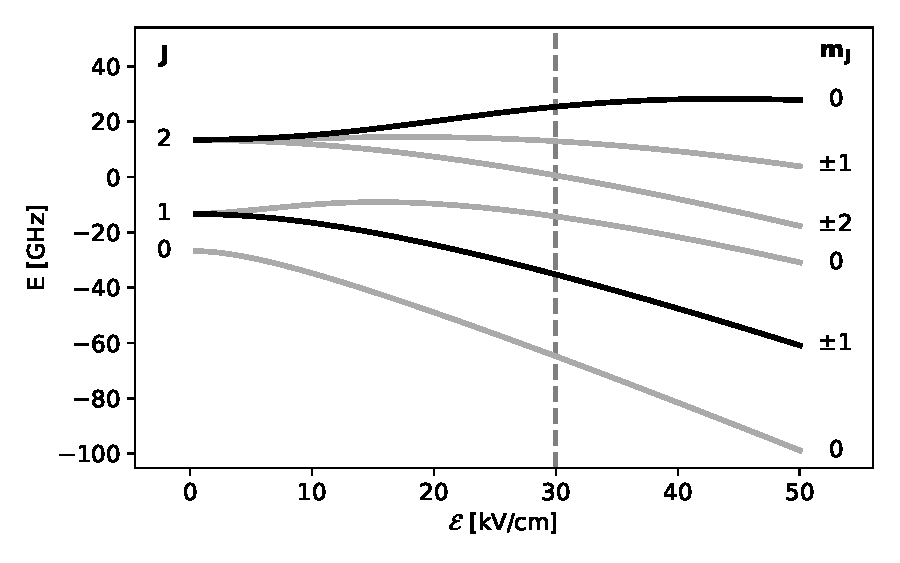
\includegraphics[width=\textwidth/2]{figs/matplotlib/low_to_high_field.pdf}
	\caption{Evolution of the energy eigenstates of the TlF Hamiltonian (Eq. \ref{eq:hyperfine_hamiltonian}) for $\Esca$ ranging from $0\,$V/cm to $50\,$kV/cm, for $J=0,1,2$. States used in \CENTREX\ are shown in bold. Hyperfine structure is unresolved in this plot.}
	\label{fig:low_to_high_field}
\end{figure}

Throughout most of the \CENTREX\ apparatus, TlF molecules experience a non-zero $\Esca$-field and (nominally) zero $\Bsca$-field.
The character of the energy eigenstates changes significantly depending on the $\Esca$-field magnitude, which varies dramatically between stages of the experiment. Hence, it is useful to describe the energy eigenstates of the TlF electronic ground state in different regimes of $\Esca$-field strength (with $\Bsca = 0$), as defined by the ratio of Stark shifts, $\Delta E_{\rm S} = \langle \mathcal{H}_{\rm S}\rangle \sim \mu_e^2 \Esca^2/B$, to the strength of hyperfine interactions, $E_{\rm hf} = \langle \mathcal{H}_{\rm sr} + \mathcal{H}_{\rm ss}\rangle \sim c_j$, or rotational energies, $E_{\rm rot} = \langle \mathcal{H}_{\rm rot}\rangle \sim B$. In all regimes, the total angular momentum projection $m_F$ along 
a space-fixed quantization axis $\hat{z}$ (always defined such that $\Evec$ is very nearly parallel to $\hat{z}$), is an exact quantum number.

In the low-field regime, where $\Delta E_{\rm S} \ll E_{\rm hf}$, energy eigenstates retain $J$, $F$, and $F_1$ as approximate quantum numbers. 
In the mid-field regime, where $E_{\rm hf} \ll \Delta E_{\rm S} \ll E_{\rm rot}$, both $J$ and $m_J$ are approximate quantum numbers. 
Here, the tensor part of the Stark shifts gives rise to energy splittings between levels with different values of $|m_J|$ that are comparable in size to the scalar shifts, i.e., of order $\Delta E_{\rm S}$.  Thus, when $m_J\neq 0$, $\vec{J}$ is strongly coupled to $\Evec$ (and hence to the molecular axis $\vec{\hat{n}}$) by this Stark interaction. In this case, each nuclear spin is coupled to $\vec{J}$ (and thus also to $\Evec$) by the spin-rotation interactions of $\mathcal{H}_{\rm sr}$. Hence, here $m_{I_1}$ and $m_{I_2}$ are approximate quantum numbers. By contrast, in states where $m_J=0$ (including when $J=0$) in this regime, $\left\langle \mathcal{H}_{\rm sr}\right\rangle$ vanishes to first order, and the nuclear spins do not couple to $\vec{J}$ and $\Evec$. However, the nuclear spins remain coupled to each other via the spin-spin interaction $\mathcal{H}_{\rm ss}$.  So, here the total nuclear spin $\vec \It = \vec I_1 + \vec I_2$ and its projection $m_{\It}$ are approximate quantum numbers in addition to $J$ and $m_J=0$. 
Finally, in the high-field regime where $E_{\rm hf} \ll E_{\rm rot} \lesssim \Delta E_{\rm S}$, $J$ states are strongly mixed, and separations between $m_J$ states are on the order of $E_{\rm rot}$. Here, eigenstates are defined by the same approximate quantum numbers as in the mid-field regime, aside from $J$. We refer to these strongly mixed states with the label $\widetilde{J}$, which corresponds to the value of $J$ that any given state connects to adiabatically, if the $\Esca$-field is reduced.
Table \ref{tab:E_field_regimes} summarizes the different regimes and associated eigenstates.  
\begin{table*}[t]
    \centering
    \def\colseplarge{4ex} % should only be used in this table
	\begin{tabular}{@{}r@{\hspace{\colseplarge}}r@{$\,\Delta E_{\rm S}\,$}l@{\hspace{\colseplarge}}r@{$\,\Esca\,$}l@{\hspace{\colseplarge}}>{\raggedright\arraybackslash}m{4cm}@{}}
    	\toprule
    	Regime & \multicolumn{2}{c}{Definition} & \multicolumn{2}{c}{Field strength} & Approx. eigenstates \\
		\midrule
		 Low
		 & & $\ll E_{\rm hf}$
		 & & $\lesssim 50 \Vcm$
		 & $\ket{J,F_1,F,m_F}$ \\\addlinespace[2ex]
		 %
	     Mid
	     & $E_{\rm hf} \ll$ & $\ll E_{\rm rot}$
	     & $50 \Vcm \ll$ & $\lesssim 5 \kVcm$
	     & $\ket{J,m_J \neq 0}\ket{m_{I_1},m_{I_2}}$ 
	       $\ket{J,m_J=0}\ket{\It,m_{\It}}$ \\\addlinespace[2ex]
	     %
	     High
	     & $E_{\rm hf} \ll E_{\rm rot} \lesssim$ &
	     & $5\kVcm \ll$ &
	     & $\ket{\widetilde{J},m_J\neq 0} \ket{m_{I_1},m_{I_2}}$
	       $\ket{\widetilde{J},m_J=0}\ket{\It,m_{\It}}$ \\
		\bottomrule
	\end{tabular}
	\caption{Regimes of electric field strength and associated eigenstates in TlF.}
	\label{tab:E_field_regimes}
\end{table*}


Figure \ref{fig:low_to_mid_field} shows how the relevant energies and eigenstates evolve from the low-field to the mid-field regime for $J=1$ and $J=2$ states.  Bold curves are states directly relevant to \CENTREX. Figure \ref{fig:low_to_high_field} shows a zoom out of states up to $J=2$ from low to high fields.

The $^{205}$Tl NSM measurement is carried out in $\tilde{J} = 1,\, m_J = \pm1$ states of TlF at large electric field $\mathcal{E} = 30$ kV/cm. This choice of states takes advantage of the structure of TlF in electric fields, in two ways. First, the observable energy shift associated with $S$, $\Delta E$, scales linearly with the degree of polarization $\mathcal{P}$ of the TlF molecule (Eq. \ref{eq:frequency_shift_due_to_NSM}). An electric field more easily polarizes states with low $J$, since $\mathcal{P}$ arises from mixing between states with different parity and thus different $J$; these states are closest together when $J$ is small. Additionally, as discussed in Sec. \ref{Sec:InternalComagnetometry}, certain dangerous systematic errors in the NSM measurement are dramatically suppressed in the presence of a strong spin-rotation interaction (later referred to as an effective intra-molecular magnetic field). This requires $m_J \neq 0$. The $\tilde{J} = 1,\, m_J = \pm1$ states hence provide the best combination of sensitivity and systematic error suppression in TlF.\footnote{$|\mathcal{P}|$ is larger in the $J=0,m_J = 0$ states, given the same $\Esca$-field value. Hence, the NSM gives larger energy shifts there. However, in these states where $m_J = 0$, the effective intra-molecular magnetic field vanishes.}
\section{Related Work} \paragraph{Sampling CF data.} Sampling in CF-data has been a popular choice for three major scenarios. Most prominently, sampling is used for mining hard-negatives while training recommendation algorithms. Some popular approaches include random sampling; using the graph-structure % to find the hardest negatives 
\cite{pinsage, eclare}; and ad-hoc techniques like similarity search \cite{slice}, stratified sampling \cite{sampling_cf_nn}, \etc % On the other hand, 
Sampling is also generally employed for evaluating recommendation algorithms by estimating expensive to compute metrics like Recall, nDCG, \etc \cite{sampled_metrics, castells_sampling}. Finally, sampling is also used to create smaller sub-samples of 
% the \emph{entire} data 
a big dataset
for reasons like fast experimentation, benchmarking different algorithms, privacy concerns, \etc However, the consequences of different samplers on any of these downstream applications is under-studied, and is the main research interest of this paper. 

\paragraph{Coreset selection.} Closest to our work, a coreset is loosely defined as a subset of data-points that maintains a similar ``quality'' as the full dataset for subsequent model training. Submodular approaches try to optimize a function $f : \mathbf{V} \mapsto \mathcal{R}_+$ which measures the utility of a subset $\mathbf{V} \subseteq \mathbf{X}$, and use it as a proxy to select the best coreset \cite{coreset_1}. More recent works treat coreset selection as a bi-level optimization problem \cite{coreset_bilevel, coreset_bilevel_2} and directly optimize for the best coreset for a given downstream task. Selection-via-proxy \cite{svp} is another technique which employs a base-model as a proxy to tag the importance of each data-point. Note, however, that 
% all of the discussed 
most existing
coreset selection approaches were designed primarily for classification data, whereas adapting them for CF-data is non-trivial because of: (1) the inherent data heterogeneity; the (2) wide range of recommendation metrics; and (3) the prevalent missing-data characteristics.

\paragraph{Evaluating sample quality.} The quality of a dataset sample, if estimated correctly is of high interest for various applications. Short of being able to evaluate the ``true'' utility of a sample, one generally resorts to either retaining task-dependent characteristics \cite{evaluate_sample_quality_1} \emph{or} employing universal, handcrafted features like a social network's hop distribution, eigenvalue distribution, \etc \cite{large_graphs} as meaningful proxies. Note that evaluating the sample quality with a limited set of handcrafted features might introduce bias in the sampled data, depending on the number and quality of such features.

\section{Sampling Collaborative Filtering Datasets} Given our motivation of quickly benchmarking recommendation algorithms, we now aim to \emph{characterize} the performance of various commonly-used sampling strategies. We loosely define the performance of a sampling scheme as 
%it's
its
ability in effectively retaining the performance-ranking of different recommendation algorithms on the full \vs sub-sampled data. In this section, we start by discussing the different recommendation feedback scenarios we consider, along with a representative sample of popular recommendation algorithms that we aim to efficiently benchmark. We then examine popular data sampling strategies, followed by proposing a novel, proxy-based sampling strategy (\sampler) that is especially suited for sampling representative subsets from long-tail CF data.

\subsection{Problem Settings \& Methods Compared} \label{feedback_types} \label{algorithms}
To give a representative sample of typical recommendation scenarios, we consider three different user feedback settings. In \emph{explicit feedback}, each user $u$ gives a numerical rating $r^u_i$ to each interacted item $i$; the model must predict these ratings for novel (test) user-item interactions. Models from this class are evaluated in terms of the Mean Squared Error (MSE) of the predicted ratings. Another scenario we consider is \emph{implicit feedback}, where the interactions for each user are only available for positive items (\eg clicks or purchases), whilst all non-interacted items are considered as negatives. We employ the AUC, Recall@$100$, and nDCG@$10$ metrics to evaluate model performance for implicit feedback algorithms. Finally, we also consider \emph{sequential feedback}, where each user $u$ interacts with an ordered sequence of items $\mathcal{S}^u = (\mathcal{S}^u_1, \mathcal{S}^u_2, \ldots, \mathcal{S}^u_{|\mathcal{S}^u|})$ such that $\mathcal{S}^u_i \in \mathcal{I}$ for all $i \in \{1, \ldots, |\mathcal{S}^u|\}$. Given $\mathcal{S} = \{ \mathcal{S}^u ~|~ \forall u \in \mathcal{U} \}$, the goal is to identify the \emph{next-item} for each sequence $\mathcal{S}^u$ that each user $u$ is most likely to interact with. We use the same metrics as in implicit feedback settings. Note that following recent warnings against sampled metrics for evaluating recommendation algorithms \cite{sampled_metrics, castells_sampling}, we compute both Recall and nDCG by ranking \emph{all} items in the dataset. Further specifics about the datasets used, pre-processing, train/test splits, \etc are discussed in-depth in \cref{main_exp}. 

Given the diversity of the scenarios discussed above, there are numerous relevant recommendation algorithms. We use the following seven recommendation algorithms, intended to represent the state-of-the-art and standard baselines:
\begin{itemize}
    \listheader{PopRec:} A na\"ive baseline that simply ranks items according to overall train-set popularity. Note that this method is unaffected by the user for which items are being recommended, and has the \emph{same global ranking} of all items.
    
    \listheader{Bias-only:} Another simple baseline that assumes no interactions between users and items. Formally, it learns: (1) a global bias $\alpha$; (2) scalar biases $\beta_u$ for each user $u \in \mathcal{U}$; and (3) scalar biases $\beta_i$ for each item $i \in \mathcal{I}$. Ultimately, the rating/relevance for user $u$ and item $i$ is modeled as $\hat{r}^u_i = \alpha + \beta_u + \beta_i$.

    \listheader{Matrix Factorization (MF) \cite{mf}:} Represents both users and items in a common, low-dimensional latent-space by factorizing the user-item interaction matrix. Formally, the rating/relevance for user $u$ and item $i$ is modeled as $\hat{r}^u_i = \alpha + \beta_u + \beta_i + \gamma_u \cdot \gamma_i$ where $\gamma_u, \gamma_i \in \mathbb{R}^d$ are learned latent representations. 
    
    \listheader{Neural Matrix Factorization (NeuMF) \cite{neural_mf}:} Leverages the representation power of deep neural-networks to capture non-linear correlations between user and item embeddings. Formally, the rating/relevance for user $u$ and item $i$ is modeled as $\hat{r}^u_i = \alpha + \beta_u + \beta_i + f(\gamma_u ~||~ \gamma_i ~||~ \gamma_u \cdot \gamma_i)$ where $\gamma_u, \gamma_i \in \mathbb{R}^d$, `||' represents the concatenation operation, and $f : \mathbb{R}^{3d} \mapsto \mathbb{R}$ represents an arbitrarily complex neural network. 
    
    \listheader{Variational Auto-Encoders for Collaborative Filtering (MVAE) \cite{mvae}:} Builds upon the Variational Auto-Encoder (VAE) \cite{vae} framework to learn a low-dimensional representation of a user's consumption history. More specifically, MVAE encodes each user's bag-of-words consumption history using a VAE and further decodes the latent representation to obtain the completed user preference over all items.
    
    \listheader{Sequential Variational Auto-Encoders for Collaborative Filtering (SVAE) \cite{svae}:} A sequential algorithm that combines the temporal modeling capabilities of a GRU \cite{gru} along with the representation power of VAEs. Unlike MVAE, SVAE uses a GRU to encode the user's consumption sequence followed by a multinomial VAE at each time-step to model the likelihood of the next item. 
    
    \listheader{Self-attentive Sequential Recommendation (SASRec) \cite{sasrec}:} Another sequential algorithm that relies on the sequence modeling capabilities of self-attentive neural networks \cite{self_attention} to predict the occurance of the 
    %next-item 
    next item
    in a user's consumption sequence. To be precise, given a user $u$ and 
    %it's
    their
    time-ordered consumption history  $\mathcal{S}^u = (\mathcal{S}^u_1, \mathcal{S}^u_2, \ldots, \mathcal{S}^u_{|\mathcal{S}^u|})$, SASRec first applies self-attention on $\mathcal{S}^u$ followed by a series of non-linear feed-forward layers to finally obtain the next item likelihood.
\end{itemize}
We also list 
%the pertinence of 
models and metrics for each of the three different CF-scenarios in \cref{model_scenario_table}. Since bias-only, MF, and NeuMF can be trained for all three CF-scenarios, we optimize them using the regularized least-squares regression loss for explicit feedback, and the pairwise-ranking (BPR \cite{bpr}) loss for implicit/sequential feedback. Note however that the aforementioned algorithms are only intended to be a representative sample of a 
%wide-pool 
wide pool
of recommendation algorithms, and in our pursuit to benchmark recommender systems faster, we are primarily concerned with the \emph{ranking} of different algorithms on the full dataset \vs a smaller sub-sample.

\begin{table*}[!ht]
    \begin{small} % normalsize, small, footnotesize
    \begin{center}
        % \begin{subtable}{0.5\linewidth}
        % \centering
        %     \begin{tabular}{c | c c c}
        %         \toprule
        %         \multirow{2}{*}{Algorithm} & \multicolumn{3}{c}{CF-scenario} \\
        %         & Explicit & Implicit & Sequential \\ \midrule
                
        %         Bias-only   & Yes & Yes & Yes \\
        %         MF          & Yes & Yes & Yes \\
        %         NeuMF       & Yes & Yes & Yes \\
        %         PopRec      & $\times$ & Yes & Yes \\
        %         MVAE        & $\times$ & Yes & Yes \\
        %         SVAE        & $\times$ & $\times$ & Yes \\
        %         SASRec      & $\times$ & $\times$ & Yes \\ \bottomrule
        %     \end{tabular}
        % \end{subtable}%
        % \begin{subtable}{0.5\linewidth}
        % \centering
        %     \begin{tabular}{c | c c c}
        %         \toprule
        %         \multirow{2}{*}{Metric} & \multicolumn{3}{c}{CF-scenario} \\
        %         & Explicit & Implicit & Sequential \\ \midrule
                
        %         MSE       & Yes & $\times$ & $\times$ \\
        %         AUC       & $\times$ & Yes & Yes \\
        %         Recall@k  & $\times$ & Yes & Yes \\
        %         nDCG@k    & $\times$ & Yes & Yes \\ \bottomrule
        %     \end{tabular}
        % \end{subtable}%
        \begin{tabular}{c | c c c c c c c | c c c c}
            \toprule
            \multirow{3}{*}{CF-scenario} & \multicolumn{7}{c|}{\emph{Algorithm}} & \multicolumn{4}{c}{\emph{Metric}} \\
            & \multicolumn{7}{c|}{} & \multicolumn{4}{c}{} \\
            & Bias-only & MF & NeuMF & PopRec & MVAE & SVAE & SASRec & MSE & AUC & Recall@k & nDCG@k \\ \midrule
            Explicit & Yes & Yes & Yes & $\times$ & $\times$ & $\times$ & $\times$ & Yes & $\times$ & $\times$ & $\times$ \\[0.6mm]
            Implicit & Yes & Yes & Yes & Yes & Yes & $\times$ & $\times$ & $\times$ & Yes & Yes & Yes \\[0.6mm]
            Sequential & Yes & Yes & Yes & Yes & Yes & Yes & Yes & $\times$ & Yes & Yes & Yes \\[0.6mm]
            \bottomrule
        \end{tabular}
    \end{center}
    \end{small}
    \bigskip
    \caption{Demonstrates the pertinence of each CF-scenario towards each algorithm (left) and each metric (right). Note that we can use ranking metrics for explicit feedback, however, we only use MSE as a design choice and due to it's direct relevance.}
    \label{model_scenario_table}
    \vspace{-6mm} %Put here to reduce too much white space after your table
\end{table*}

\subsection{Sampling Strategies} \label{common_sampling_schemes}
Given a user-item CF dataset \dataset, we aim to create a $p\%$ subset $\mathcal{D}^{s, p}$ according to some sampling strategy $s$. In this paper, to be comprehensive, we consider a sample of eight popular sampling strategies, which can be grouped into the following three categories:

\subsubsection{Interaction sampling. \ \ } We first discuss three strategies that sample interactions from \dataset. In \emph{Random Interaction Sampling}, we generate $\mathcal{D}^{s, p}$ by randomly sampling $p\%$ of all the user-item interactions in \dataset. \emph{User-history Stratified Sampling} is another popular sampling technique (see \eg \cite{svae, handbook}) to generate smaller CF-datasets. To match the user-frequency distribution amongst \dataset and $\mathcal{D}^{s, p}$, it randomly samples $p\%$ of interactions from each user's consumption history. Unlike random stratified sampling, \emph{User-history Temporal Sampling} samples $p\%$ of the \emph{most recent} interactions for each user. This strategy is representative of the popular practice of making data subsets from the online traffic of the last $x$ days \cite{eclare, pfastre}.

\subsubsection{User sampling. \ \ } Similar to sampling interactions, we also consider two strategies which sample users in \dataset instead. To ensure a fair comparison amongst the different kinds of sampling schemes used in this paper, we retain exactly $p\%$ of the \emph{total interactions} in $\mathcal{D}^{s, p}$. In \emph{Random User Sampling}, we retain users from \dataset at random. To be more specific, we iteratively preserve \emph{all} the interactions for a random user until we have retained $p\%$ of the original interactions. Another strategy we employ is \emph{Head User Sampling}, in which we iteratively remove the user with the least amount of total interactions. This method is representative of commonly used data pre-processing strategies (see \eg \cite{mvae, neural_mf}) to make data suitable for parameter-heavy algorithms. Sampling the data in such a way can introduce bias toward users from minority groups which might raise concerns from a diversity and fairness perspective \cite{fairness}.

\subsubsection{Graph sampling. \ \ } Instead of sampling directly from \dataset, we also consider three strategies that sample from the inherent user-item bipartite interaction graph $\mathcal{G}$. In \emph{Centrality-based Sampling}, we proceed by computing the pagerank centrality scores \cite{pagerank} for each node in $\mathcal{G}$, and retain all the edges (interactions) of the \emph{top scoring nodes} until a total $p\%$ of the original interactions have been preserved. Another popular strategy we employ is \emph{Random-walk Sampling} \cite{large_graphs}, which performs multiple random-walks with restart on $\mathcal{G}$ and retains the edges amongst those pairs of nodes that have been visited at least once. We keep expanding our walk until $p\%$ of the initial edges have been retained. We also utilize \emph{Forest-fire Sampling} \cite{forest_fire}, which is a snowball sampling method and proceeds by randomly ``burning'' the outgoing edges of visited nodes. It initially starts with a random node, and then propagates to a random subset of previously unvisited neighbors. The propagation is terminated once we have created a graph-subset with $p\%$ of the initial edges.

\subsection{\sampler: Selection-Via-Proxy for CF data} \label{svp_cf} 
Selection-Via-Proxy (SVP) \cite{svp} is a leading coreset mining technique for classification datasets like CIFAR10 \cite{cifar} and ImageNet \cite{image_net}. The main idea proposed is simple and effective, and proceeds by training a relatively inexpensive base-model as a proxy to define the ``importance'' of a data-point. However, applying SVP to CF-data can be highly non-trivial because of the following impediments:
\begin{itemize}
    \listheader{Data heterogeneity:} Unlike classification data 
    % $\mathcal{D}_c = \left\{ (x, y) ~|~ x \in \mathbb{R}^d, y\in \mathcal{Y}\right\}$ 
    over some input space $\mathcal{X}$ and label-space $\mathcal{Y}$, CF-data consists of numerous four-tuples $\{u, i, r^u_i, t^u_i\}$. Such multimodal data adds many different dimensions to sample data from, making it increasingly complex to define meaningful samplers. 
    
    \listheader{Defining the importance of a data point:} Unlike classification, where we can measure the performance of a classifier by 
    %it's
    its
    empirical risk on held-out data, for recommendation, there are a variety of different scenarios (\cref{feedback_types}) along with a wide list of relevant evaluation metrics. Hence, it becomes challenging to adapt importance-tagging techniques like greedy k-centers \cite{k_centers}, forgetting-events \cite{forgetting_events}, \etc for recommendation tasks.
    
    \listheader{Missing data:} 
    CF-data is well-known for (1) 
    %it's 
    its
    sparsity; (2) skewed and long-tail user/item distributions; and (3) missing-not-at-random (MNAR) properties of the user-item interaction matrix. This results in additional problems as we are now sampling data from skewed, MNAR data, especially using proxy-models trained on the same skewed data. Such sampling in the worst-case might even lead to exacerbating existing biases in the data or even aberrant data samples.
\end{itemize}
To address these fundamental limitations in applying the SVP philosophy to CF-data, we propose \sampler to sample representative subsets from large user-item interaction data. \sampler is also specifically devised for our objective of benchmarking different recommendation algorithms, as it relies on the crucial assumption that the ``easiest'' part of a dataset will generally be easy \emph{for all} algorithms. Under this assumption, even after removing such data we are still likely to retain the overall algorithms' ranking.

Because of the inherent data heterogeneity in user-item interaction data, we can sub-sample in a variety of different ways. We design \sampler to be versatile in this aspect as it can be applied to sample users, items, interactions, or combinations of them, by marginally adjusting the definition of importance of each data-point. In this paper, we limit the discussion to only sampling users and interactions (separately), but extending \sampler for sampling across other data modalities should be relatively straightforward.

Irrespective of whether to sample users or interactions, \sampler proceeds by training an inexpensive proxy model $\mathcal{P}$ on the full, original data \dataset and modifies the forgetting-events approach \cite{forgetting_events} to retain the points with the \emph{highest} importance. To be more specific, for explicit feedback, we define the importance of each data-point \ie $\{u, i, r^u_i, t^u_i\}$ interaction as $\mathcal{P}$'s average MSE (over epochs) of the specific interaction if we're sampling interactions \emph{or} $\mathcal{P}$'s average MSE of $u$ (over epochs) if we're sampling users. Whereas, for implicit and sequential feedback, we use $\mathcal{P}$'s average inverse-AUC while computing the importance of each data-point. For the sake of completeness, we experiment with both Bias-only and MF as two different kinds of proxy-models for \sampler. Since both models can be trained for all three CF-scenarios (\cref{model_scenario_table}), we can directly use them to tag the importance for each CF-scenario.

Ultimately, to handle the MNAR and long-tail problems, we also propose \samplerprop which employs user and item propensities to correct the distribution mismatch while estimating the importance of each datapoint. More specifically, let $p_{u, i} = P(r^u_i = 1 ~|~ \overstar{r}^u_i = 1)$ denote the probability of user $u$ and item $i$'s interaction actually being observed (propensity), $E$ be the total number of epochs that $\mathcal{P}$ was trained for, $\mathcal{P}_e$ denote the proxy model after the $e^{\mathit{th}}$ epoch, $\mathcal{I}_u^+ \coloneqq \{ j ~|~ r^u_j > 0 \}$ be the set of positive interactions for $u$, and $\mathcal{I}_u^- \coloneqq \{ j ~|~ r^u_j = 0 \}$ be the set of negative interactions for $u$; then, the importance function for \samplerprop, $\mathcal{I}_p$ is defined as follows:
\begin{align*}
% \begin{gathered}
    \mathcal{I}_p(u ~|~ \mathcal{P}) \coloneqq \frac{1}{|\mathcal{I}_u^+|} \cdot \sum_{i \in \mathcal{I}_u^+} \mathcal{I}_p(u, i ~|~ \mathcal{P}) \hspace{0.63em} ; \hspace{0.63em}
    \mathcal{I}_p(u, i ~|~ \mathcal{P}) \coloneqq \frac{\Delta(u, i ~|~ \mathcal{P})}{p_{u, i}} \\
    %where, 
% \end{gathered}
\end{align*}
\vspace{-0.6cm}
\begin{equation*}
\begin{gathered}
    \text{where,}
    \qquad \Delta(u, i ~|~ \mathcal{P}) \coloneqq 
    \begin{dcases} 
      ~~ \sum_{e=1}^{E} \left(\mathcal{P}_e(u, i) - r^u_i\right)^2 \\  %& \, \text{for explicit feedback} \\
      ~~ \text{(for explicit feedback)} \\ \\
      ~~ \sum_{e=1}^{E} \sum_{j \sim \mathcal{I}_u^-} \frac{1}{\mathds{1}\left(\mathcal{P}_e(u, i) > \mathcal{P}_e(u, j)\right)} \\ % & \, \text{for implicit/sequential feedback}
      ~~ \text{(for implicit/sequential feedback)}
   \end{dcases}
\end{gathered}
\end{equation*}
\vspace{0.1cm}

\begin{proposition}
Given an ideal propensity-model $p_{u, i}; \ \mathcal{I}_p(u, i ~|~ \mathcal{P})$ is an unbiased estimator of $\Delta(u, i ~|~ \mathcal{P})$.
\end{proposition}

\begin{proof}
\begin{align*}
    \EE_{u \sim \mathcal{U}} \EE_{i \sim \mathcal{I}} \left[ \mathcal{I}_p(u, i ~|~ \mathcal{P}) \right] \hspace{5.65cm}
\end{align*}
\vspace{-0.4cm}
\begin{align*}
    &= \frac{1}{|\mathcal{U}| |\mathcal{I}|} \sum_{u \sim \mathcal{U}} \sum_{i \sim \mathcal{I}} \mathcal{I}_p(u, i ~|~ \mathcal{P}) \cdot P(r_i^u = 1) \\
    % &= \frac{1}{|\mathcal{U}| \cdot |\mathcal{I}|} \sum_{u \sim \mathcal{U}} \sum_{i \sim \mathcal{I}} \mathcal{I}_p(u, i ~|~ \mathcal{P}) \cdot \left( P(r_i^u = 1, \overstar{r}_i^u = 0) ~+~ P(r_i^u = 1, \overstar{r}_i^u = 1) \right) \\
    &= \begin{aligned}[t]
        \frac{1}{|\mathcal{U}| |\mathcal{I}|} \sum_{u \sim \mathcal{U}} \sum_{i \sim \mathcal{I}} \frac{\Delta(u, i ~|~ \mathcal{P})}{p_{u, i}} \cdot ( P(\overstar{r}_i^u = 0) \cdot \cancelto{0}{P(r_i^u = 1 ~|~ \overstar{r}_i^u = 0)} \\
        +~ P(\overstar{r}_i^u = 1) \cdot P(r_i^u = 1 ~|~ \overstar{r}_i^u = 1)) \\ % \hspace{3.6cm} \\
        % \text{(One-sided label noise)} \\
    \end{aligned} \\
    &= \frac{1}{|\mathcal{U}| |\mathcal{I}|} \sum_{u \sim \mathcal{U}} \sum_{i \sim \mathcal{I}} \Delta(u, i ~|~ \mathcal{P}) \cdot P(\overstar{r}_i^u = 1) \\ %\hspace{0.5cm} 
    &= \EE_{u \sim \mathcal{U}} \EE_{i \sim \mathcal{I}} \left[ \Delta(u, i ~|~ \mathcal{P}) \right] \qedhere
\end{align*}
\end{proof} 

\paragraph{Propensity model.} A wide variety of ways exist 
%in the literature 
to model the propensity score of a user-item interaction \cite{propensity_1, rec_as_treatments, sachdeva_kdd20, pfastre}. The most common ways comprise using machine learning models like na\"ive bayes and logistic regression \cite{rec_as_treatments}, or by fitting handcrafted functions \cite{pfastre}. For our problem statement, we make a simplifying assumption that the data noise is one-sided \ie $P(r^u_i = 1 ~|~ \overstar{r}^u_i = 0)$ or the probability of a user interacting with a \emph{wrong} item is \emph{zero}, and model the probability of an interaction going missing to decompose over the user and item as follows:
\begin{align*}
    p_{u, i} &= P(r^u_i = 1 ~|~ \overstar{r}^u_i = 1) \\
    &= P(r^u = 1 ~|~ \overstar{r}^u = 1) \cdot P(r_i = 1 ~|~ \overstar{r}_i = 1) ~=~ p_u \cdot p_i
\end{align*}
% \begin{equation}
%     p_{u, i} \ \ = \ \ P(r^u_i = 1 ~|~ \overstar{r}^u_i = 1)
%     \ \ = \ \ P(r^u = 1 ~|~ \overstar{r}^u = 1) \cdot P(r_i = 1 ~|~ \overstar{r}_i = 1) 
%     \ \ = \ \ p_u \cdot p_i
% \end{equation}
Ultimately, following \cite{pfastre}, we assume the user and item propensities to lie on the following sigmoid curves:
\begin{equation*}
\begin{split}
    p_u \coloneqq \frac{1}{1 + C_u \cdot e^{-A \cdot log(N_u + B)}} \quad ; \quad p_i \coloneqq \frac{1}{1 + C_i \cdot e^{-A \cdot log(N_i + B)}}
\end{split}
\end{equation*}
Where, $N_u$ and $N_i$ represent the total number of interactions of user $u$ and item $i$ respectively, $A$ and $B$ are two fixed scalars, $C_u = (log(|\mathcal{U}|) - 1) \cdot (B+1)^A$ and $C_i = (log(|\mathcal{I}|) - 1) \cdot (B+1)^A$. 

\subsection{Performance of a sampling strategy} \label{sampling_perf}
% Preserving \emph{exactly} the same levels of performance on sub-sampled data over metrics like MSE, AUC, \etc is a very challenging problem. However, a simpler albeit useful problem is accurately preserving the \emph{ranking} of different algorithms on sub-sampled data. For \eg, a sampling scheme that has a very low bias but high variance in preserving metric performance values has a lesser utility than a different sampling scheme with high amounts of bias but low variance, since the algorithm ranking is still preserved and can be used to benchmark models much faster. With the following notion in mind, to 
To quantify the performance of a sampling strategy $s$ on a dataset $\mathcal{D}$, we start by creating various $p\%$ subsets of $\mathcal{D}$ according to $s$ and call them $\mathcal{D}^{s, p}$. Next, we train and evaluate all the relevant recommendation algorithms on both $\mathcal{D}$ and $\mathcal{D}^{s, p}$. Let the \emph{ranking} of all algorithms according to CF-scenario $f$ and metric $m$ trained on $\mathcal{D}$ and $\mathcal{D}^{s, p}$ be $\mathcal{R}_{f, m}$ and $\mathcal{R}^{s, p}_{f, m}$ respectively, then the performance measure $\Psi(\mathcal{D}, s)$ is defined as the average correlation between $\mathcal{R}_{f, m}$ and $\mathcal{R}^{s, p}_{f, m}$ measured through Kendall's Tau over all possible CF-scenarios, metrics, and sampling percents:
\begin{equation*}
\begin{split}
    \Psi\left(\mathcal{D}, s\right) &= \lambda \cdot \sum_{f} \sum_{m} \sum_{p} \tau\left(\mathcal{R}_{f, m}, \mathcal{R}^{s, p}_{f, m}\right) \\
    % &= \lambda \cdot \sum_{f} \sum_{m} \sum_{p} \frac{2}{n \cdot (n-1)} \sum_{i < j} \mathds{1}\left(\mathcal{R}_{f, m}(i) - \mathcal{R}_{f, m}(j)\right) \cdot \mathds{1}\left(\mathcal{R}^{s, p}_{f, m}(i) - \mathcal{R}^{s, p}_{f, m}(j)\right)
\end{split}
\end{equation*}
Where $\lambda$ is an appropriate normalizing constant for computing the average, sampling percent $p \in \{ 80, 60, 40, 20, 10, 1 \}$, CF-scenario $f$, metric $m$ and their pertinence towards each other can all be found in \cref{model_scenario_table}. $\Psi$ has the same range as Kendall's Tau \ie $[-1, 1]$ and a higher $\Psi$ indicates strong agreement between the algorithm ranking on the full and sub-sampled datasets, whereas a large negative $\Psi$ implies that the algorithm order was effectively reversed.

\subsection{Experiments} \label{main_exp}

\paragraph{Datasets.} To promote dataset diversity in our experiments, we use six public user-item rating interaction datasets with varying sizes, sparsity patterns, and other characteristics. We use the Magazine, Luxury, and Video-games categories of the Amazon review dataset \cite{amz_data}, along with the Movielens-100k \cite{movielens}, BeerAdvocate \cite{beer_dataset}, and GoodReads Comics \cite{mengting_goodreads} datasets. A brief set of data statistics is also presented in \cref{data_stats}. We simulate all three CF-scenarios (\cref{feedback_types}) 
% for each dataset 
via different pre-processing strategies. For explicit and implicit feedback, we follow a randomized 80/10/10 train-test-validation split for each user's consumption history in the dataset, and make use of the leave-one-last \cite{train_test_splitting} strategy for sequential feedback \ie
% leave the last interaction in each user's time-sorted consumption history as a testing-point and the second last interaction as a validation-point. 
keep the last two interactions in each user's time-sorted consumption history in the validation and test-set respectively.
Since we can't control the initial construction of datasets, and to minimize the initial data bias, we follow the least restrictive data pre-processing \cite{making_progress, sigir20}. We only weed out the users 
% that have lesser 
with less
than 3 interactions,
% in total, in order 
to keep at least one occurrence 
% per user 
in the train, validation, and test sets.

\begin{table}[!ht]
    % \vspace{-1mm} %Put here to reduce too much white space after your table
    \begin{footnotesize} % normalsize, small, footnotesize
    \begin{center}
        \begin{tabular}{c | c c c c}
            \toprule
            \multirow{2}{*}{\textbf{Dataset}} & \textbf{\#} & \textbf{\#} & \textbf{\#} & \textbf{Avg. User} \\ 
            & \textbf{Interactions} & \textbf{Users} & \textbf{Items} & \textbf{history length} \\
            \midrule
            
            Amazon Magazine      & 12.7k & 3.1k  & 1.3k  & 4.1 \\
            ML-100k              & 100k  & 943   & 1.7k  & 106.04 \\
            Amazon Luxury        & 126k  & 29.7k & 8.4k  & 4.26 \\
            Amazon Video-games   & 973k  & 181k  & 55.3k & 5.37 \\
            BeerAdvocate         & 1.51M & 18.6k & 64.3k & 81.45 \\
            Goodreads Comics     & 4.37M & 133k  & 89k   & 32.72 \\
            
            \bottomrule
        \end{tabular}
    \end{center}
    \end{footnotesize}
    \vspace{2mm}
    \caption{Data statistics of the \emph{six} datasets used in this paper.}
    \label{data_stats}
    \vspace{-6mm} %Put here to reduce too much white space after your table
\end{table}

\paragraph{Training details.} We implement all algorithms in PyTorch\footnote{Code is available at \href{https://github.com/noveens/sampling_cf}{\color{blue}{https://github.com/noveens/sampling\_cf}}} 
and train on a single GPU. For a fair comparison across algorithms, we perform 
%a generous 
hyper-parameter search on the validation set. 
For the three smallest datasets used in this paper (\cref{data_stats}), we search the latent size in $\{ 4, 8, 16, 32, 50 \}$, dropout in $\{ 0.0, 0.3, 0.5 \}$, and the learning rate in $\{ 0.001, 0.006, 0.02 \}$. Whereas for the three largest datasets, we fix the learning rate to be $0.006$. % and only search over the latent-size and dropout values. 
Note that despite the limited number of datasets and recommendation algorithms used in this study, given that we need to train all algorithms with hyper-parameter tuning for all CF scenarios, $\%$ data sampled according to all different sampling strategies discussed in \cref{common_sampling_schemes}, there are a total of 
% $6 \times 3 \times 7 \times 16 \times 7 \times 30 \approx 400k$ 
$\sim400k$ 
unique models trained, 
% resulting in 
equating to
a cumulative train time of over $400k ~ \times \sim1 \text{min} \approx 9$ months.

\paragraph{Data sampling.} To compute the $\Psi$-values as defined in \cref{sampling_perf}, we construct $\{ 80, 60, 40, 20, 10, 1 \} \%$ samples for each dataset and sampling strategy. To keep comparisons as fair as possible, for all sampling schemes, we only sample on the train set and never touch the validation and test sets. % This simulates the practical scenario of sampling data only while benchmarking algorithms offline, whereas the live (test-set) traffic still remains the same.

\subsubsection{How do different sampling strategies compare to each other? \ \ } Results with $\Psi$-values for all sampling schemes on all datasets are in \cref{psi_results}. Even though there are only six datasets under consideration, there are a few prominent patterns. First, the average $\Psi$ for most sampling schemes is around $0.4$, which implies a statistically significant correlation between the ranking of algorithms on the full \vs sub-sampled datasets. Next, \sampler generally outperforms all commonly used sampling strategies by some margin in retaining the ranking of different recommendation algorithms. Finally, the methods that discard the tail of a dataset (head-user and centrality-based) are the worst performing strategies overall, which supports the recent warnings against dense sampling of data \cite{sigir20}.

\newcommand{\STAB}[1]{\begin{tabular}{@{}c@{}}#1\end{tabular}}
\begin{table*}%[!ht]
    \begin{footnotesize}
    \begin{center}
        \begin{tabular}{c c | c c c c c c | c}
            \toprule
            \multicolumn{2}{c|}{\multirow{4}{*}{\textbf{Sampling strategy}}} & \multicolumn{6}{c|}{\emph{Datasets}} & \\
            & & \multicolumn{6}{c|}{} & \\
            & & \begin{tabular}{@{}c@{}}\textbf{Amazon}\\\textbf{Magazine}\end{tabular} & \textbf{ML-100k} & \begin{tabular}{@{}c@{}}\textbf{Amazon}\\\textbf{Luxury}\end{tabular} & \begin{tabular}{@{}c@{}}\textbf{Amazon}\\\textbf{Video-games}\end{tabular} & \textbf{BeerAdvocate} & \begin{tabular}{@{}c@{}}\textbf{Goodreads}\\\textbf{Comics}\end{tabular} & \textbf{\emph{Average}} \\
            \midrule
            
            \multirow{8}{*}{\STAB{\rotatebox[origin=c]{90}{\begin{tabular}{@{}c@{}}Interaction sampling\\\end{tabular}}}} & Random & 0.428     &  0.551     &  0.409     &  0.047     &  0.455     &  0.552     &  0.407 \\[0.6mm]
            & Stratified & 0.27      &  0.499     &  0.291     &  -0.01     &  0.468     &  0.538     &  0.343 \\[0.6mm]
            & Temporal & 0.289     &  0.569     &  0.416     &  -0.02     &  \underline{0.539}     &  0.634     &  0.405 \\[0.6mm]
            & \sampler \emph{w/} MF & 0.418     &  0.674     &  0.398     &  0.326     &  0.425     &  \underline{0.662}     &  \underline{0.484} \\[0.6mm]
            & \sampler \emph{w/} Bias-only & 0.38      &  0.684     &  \underline{0.431}     &  \underline{0.348}     &  0.365     &  0.6       &  0.468 \\[0.6mm]
            & \samplerprop \emph{w/} MF & 0.381     &  0.617     &  0.313     &  0.305     &  0.356     &  0.608     &  0.43 \\[0.6mm]
            & \samplerprop \emph{w/} Bias-only & 0.408     &  0.617     &  0.351     &  0.316     &  0.437     &  0.617     &  0.458 \\[0.6mm]
            \midrule
            \multirow{7}{*}{\STAB{\rotatebox[origin=c]{90}{\begin{tabular}{@{}c@{}}User sampling\\\end{tabular}}}} & Random & 0.436     &  0.622     &  0.429     &  0.17      &  0.344     &  0.582     &  0.431 \\[0.6mm]
            & Head & 0.369     &  0.403     &  0.315     &  0.11      &  -0.04     &  -0.02     &  0.19 \\[0.6mm]
            & \sampler \emph{w/} MF & 0.468     &  0.578     &  0.308     &  0.13      &  0.136     &  0.444     &  0.344 \\[0.6mm]
            & \sampler \emph{w/} Bias-only & 0.49      &  0.608     &  0.276     &  0.124     &  0.196     &  0.362     &  0.343 \\[0.6mm]
            & \samplerprop \emph{w/} MF & 0.438 &  0.683 &  0.307 &  0.098 &  0.458 &  0.592 &  0.429 \\[0.6mm]
            & \samplerprop \emph{w/} Bias-only & 0.434     &  \underline{0.751}     &  0.233     &  0.107     &  0.506     &  0.637     &  0.445 \\[0.6mm]
            \midrule
            \multirow{4}{*}{\STAB{\rotatebox[origin=c]{90}{\begin{tabular}{@{}c@{}}Graph\\\end{tabular}}}} & Centrality & 0.307     &  0.464     &  0.407     &  0.063     &  0.011     &  0.343     &  0.266 \\[0.6mm]
            & Random-walk & \underline{0.596}  &  0.5       &  0.395     &  0.306     &  0.137     &  0.442     &  0.396 \\[0.6mm]
            & Forest-fire & 0.564  &  0.493   &  0.415   &  0.265   &  0.099  &  0.454  &  0.382 \\[0.6mm]
            \bottomrule
        \end{tabular}
        % \begin{tabular}{c || c c c | c c | c c c}
        %     \toprule
        %     \multirow{3}{*}{Dataset} & \multicolumn{3}{c|}{Interaction sampling} & \multicolumn{2}{c|}{User sampling} & \multicolumn{3}{c}{Graph sampling} \\
        %     \multirow{2}{*}{} & \multicolumn{3}{c|}{} & \multicolumn{2}{c|}{} & \multicolumn{3}{c}{} \\
        %     & Random & Stratified & Temporal & Random & Head & Centrality & RW & FF \\ \midrule \midrule
            
        %     Amazon Magazine     & 0.428    & 0.27     & 0.289    & 0.436    & 0.369    & 0.307    & \underline{0.596} & 0.564 \\
        %     ML-100k             & 0.551    & 0.499    & 0.569    & 0.622    & 0.403    & 0.464    & 0.5      & 0.493 \\
        %     Amazon Luxury       & 0.409    & 0.291    & 0.416    & 0.429    & 0.315    & 0.407    & 0.395    & 0.415 \\
        %     Amazon Video-games  & 0.047    & -0.01    & -0.02    & 0.17     & 0.11     & 0.063    & 0.306    & 0.265 \\
        %     BeerAdvocate        & 0.455    & 0.468    & \underline{0.539}    & 0.344    & -0.04    & 0.011    & 0.137    & 0.099 \\
        %     Goodreads Comics    & 0.552    & 0.538    & 0.634    & 0.582    & -0.02    & 0.343    & 0.442    & 0.454 \\ \midrule
        %     Average             & 0.407    & 0.343    & 0.405    & 0.431    & 0.19     & 0.266    & 0.396    & 0.382 \\ \bottomrule 
        % \end{tabular}
        % \newline
        % \vspace*{0.5 cm}
        % \newline
        % \begin{tabular}{c || c c c c | c c c c}
        %     \toprule
        %     \multirow{4}{*}{Dataset} & \multicolumn{4}{c|}{Interaction sampling} & \multicolumn{4}{c}{User sampling} \\
        %     \multirow{2}{*}{} & \multicolumn{4}{c|}{} & \multicolumn{4}{c}{} \\
        %     & SVP-CF & SVP-CF-Prop & SVP-CF & SVP-CF-Prop & SVP-CF & SVP-CF-Prop & SVP-CF & SVP-CF-Prop \\
        %     & Bias-only & Bias-only & MF & MF & Bias-only & Bias-only & MF & MF \\ \midrule \midrule
            
        %     Amazon Magazine     & 0.38     & 0.408    & 0.418    & 0.381    & 0.49     & 0.434    & 0.468    & 0.438 \\
        %     ML-100k             & 0.684    & 0.617    & 0.674    & 0.617    & 0.608    & \underline{0.751}    & 0.578    & 0.683 \\
        %     Amazon Luxury       & \underline{0.431}    & 0.351    & 0.398    & 0.313    & 0.276    & 0.233    & 0.308    & 0.307 \\
        %     Amazon Video-games  & \underline{0.348}    & 0.316    & 0.326    & 0.305    & 0.124    & 0.107    & 0.13     & 0.098 \\
        %     BeerAdvocate        & 0.365    & 0.437    & 0.425    & 0.356    & 0.196    & 0.506    & 0.136    & 0.458 \\
        %     Goodreads Comics    & 0.6      & 0.617    & \underline{0.662}    & 0.608    & 0.362    & 0.637    & 0.444    & 0.592 \\ \midrule 
        %     Average             & 0.468    & 0.458    & \underline{0.484}    & 0.43     & 0.343    & 0.445    & 0.344    & 0.429 \\ \bottomrule
        % \end{tabular}
    \end{center}
    \end{footnotesize}
    \bigskip
    \caption{$\Psi$-values for all datasets and sampling strategies. Higher $\Psi$ is better. The best $\Psi$ for every dataset is \underline{underlined}. The $\Psi$-values for each sampling scheme \emph{averaged over all datasets} is appended to the right.}
    \label{psi_results}
    \vspace{-6mm} %Put here to reduce too much white space after your table
\end{table*}

\subsubsection{How does the relative performance of algorithms change as a function of sampling rate? \ \ } In an attempt to better understand the impact of sampling on different recommendation algorithms used in this study (\cref{algorithms}), we visualize the probability of a recommendation algorithm moving up in the overall method ranking with data sampling. We estimate the aforementioned probability using Maximum-Likelihood-Estimation (MLE) on the experiments already run in computing $\Psi(\mathcal{D}, s)$. Formally, given a recommendation algorithm $r$, CF-scenario $f$, and data sampling percent $p$:
\begin{equation*}
    P_{\mathit{MLE}}(r ~|~ f, p) = \lambda \cdot \sum_{\mathcal{D}} \sum_{s} \sum_{m} 0.5 + \frac{\mathcal{R}_{f, m}(r) - \mathcal{R}_{f, m}^{s, p}(r)}{2 \cdot (n-1)}
\end{equation*}
where $\lambda$ is an appropriate normalizing constant, and $n$ represents the total number of algorithms. A heatmap visualizing $P_{\mathit{MLE}}$ for all algorithms and CF-scenarios is shown in \cref{percent_sampling_vs_method}. We see that simpler methods like Bias-only and PopRec have the highest probability across data scenarios of increasing their ranking order with extreme sampling. Whereas parameter-heavy algorithms like SASRec, SVAE, MVAE, \etc tend to decrease in the ranking order, which is indicative of overfitting on smaller data samples.
\begin{figure}[ht!]     
    \centering
    \vspace{-0.1cm}
    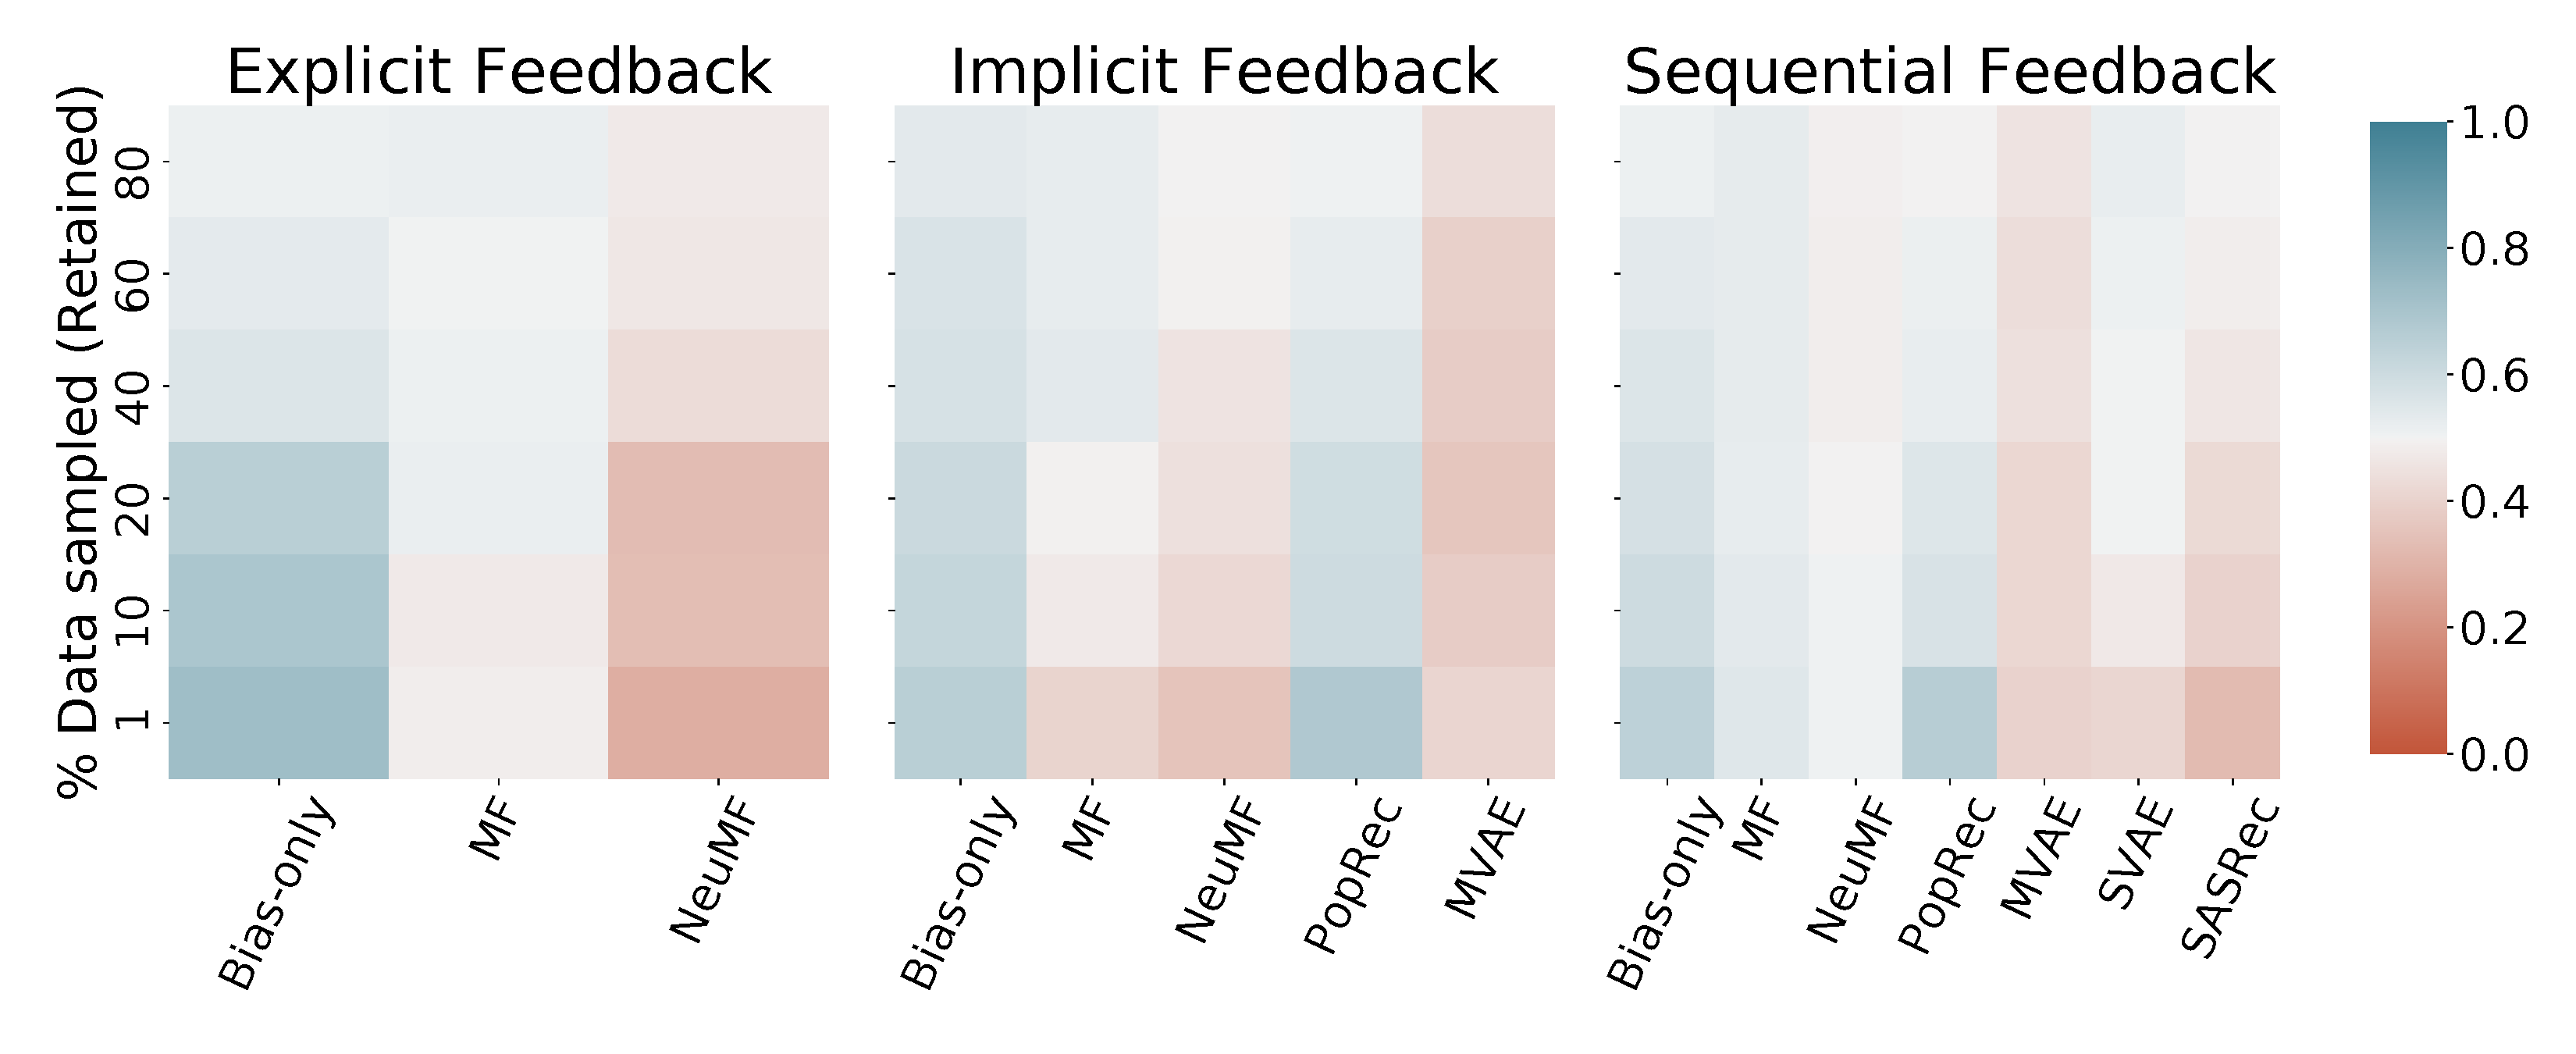
\includegraphics[width=0.9\linewidth]{figures/percent_sampling_vs_method.pdf}
    \vspace{-0.4cm}
    \caption{Heatmap of the probability of an algorithm moving in the overall ranking with extreme sampling. A high value indicates that the algorithm is most probable to \emph{move up} in the sampled data ranking order, whereas a low value indicates that the algorithm is most probable to \emph{move down}.}
    \label{percent_sampling_vs_method}
    \vspace{-0.3cm}
\end{figure}

\subsubsection{How much data to sample? \ \ } Since $\Psi$ is averaged over all $p \in \{ 80, 60, 40, 20, 10, 1 \}$\% data samples, to better estimate a reasonable amount of data to sample, we stratify $\Psi$ according to each value of $p$ and note the average Kendall's Tau. As we observe from \cref{percent_sampling_vs_tau}, %there is an expected, 
there is a steady increase in the performance measure when more data is retained. Next, despite the results in \cref{percent_sampling_vs_tau} being averaged over \emph{sixteen} sampling strategies, we still notice a significant amount of performance retained after sampling just $50-60\%$ of the data. % This holds to show that sampled data in some conditions can accurately reflect true algorithm performance.
\begin{figure}[ht!] 
    \centering
    \vspace{-0.2cm}
    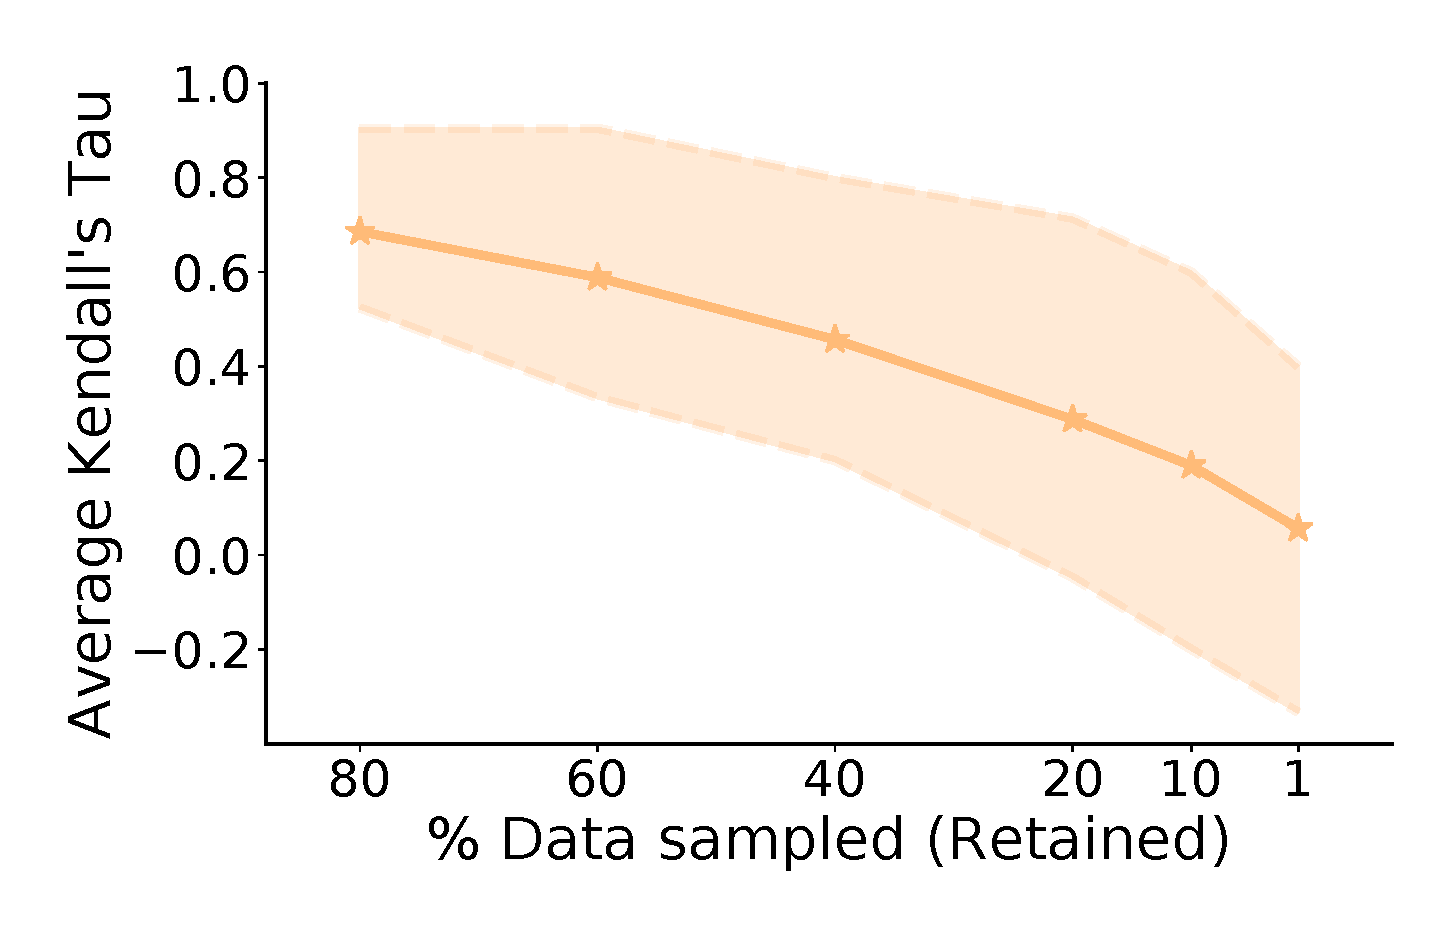
\includegraphics[width=0.6\linewidth]{figures/percent_sampling_vs_tau.pdf}
    \vspace{-0.25cm}
    \caption{Comparison of the average Kendall's Tau with \% data sampled. A higher Tau indicates better retaining power of the ranking of different recommendation algorithms.}
    \label{percent_sampling_vs_tau}
    \vspace{-0.3cm}
\end{figure} 

\subsubsection{Are different metrics affected equally by sampling? \ \ } In an attempt to better understand how the different implicit and sequential feedback metrics (\cref{feedback_types}) are affected by sampling, we visualize the average Kendall's Tau for all sampling strategies (except \sampler for brevity) and all \% data sampling choices separately over the AUC, Recall, and nDCG metrics in \cref{metric_correlation}. As expected, we observe a steady decrease in the model quality across the accuracy metrics over the different sampling schemes. This is in agreement with the analysis from \cref{percent_sampling_vs_tau}. Next, most sampling schemes follow a \emph{similar} downwards trend in performance for the three metrics with AUC being slightly less affected and nDCG being slightly more affected by extreme sampling.
\begin{figure}[ht!] 
    \vspace{-0.1cm}
    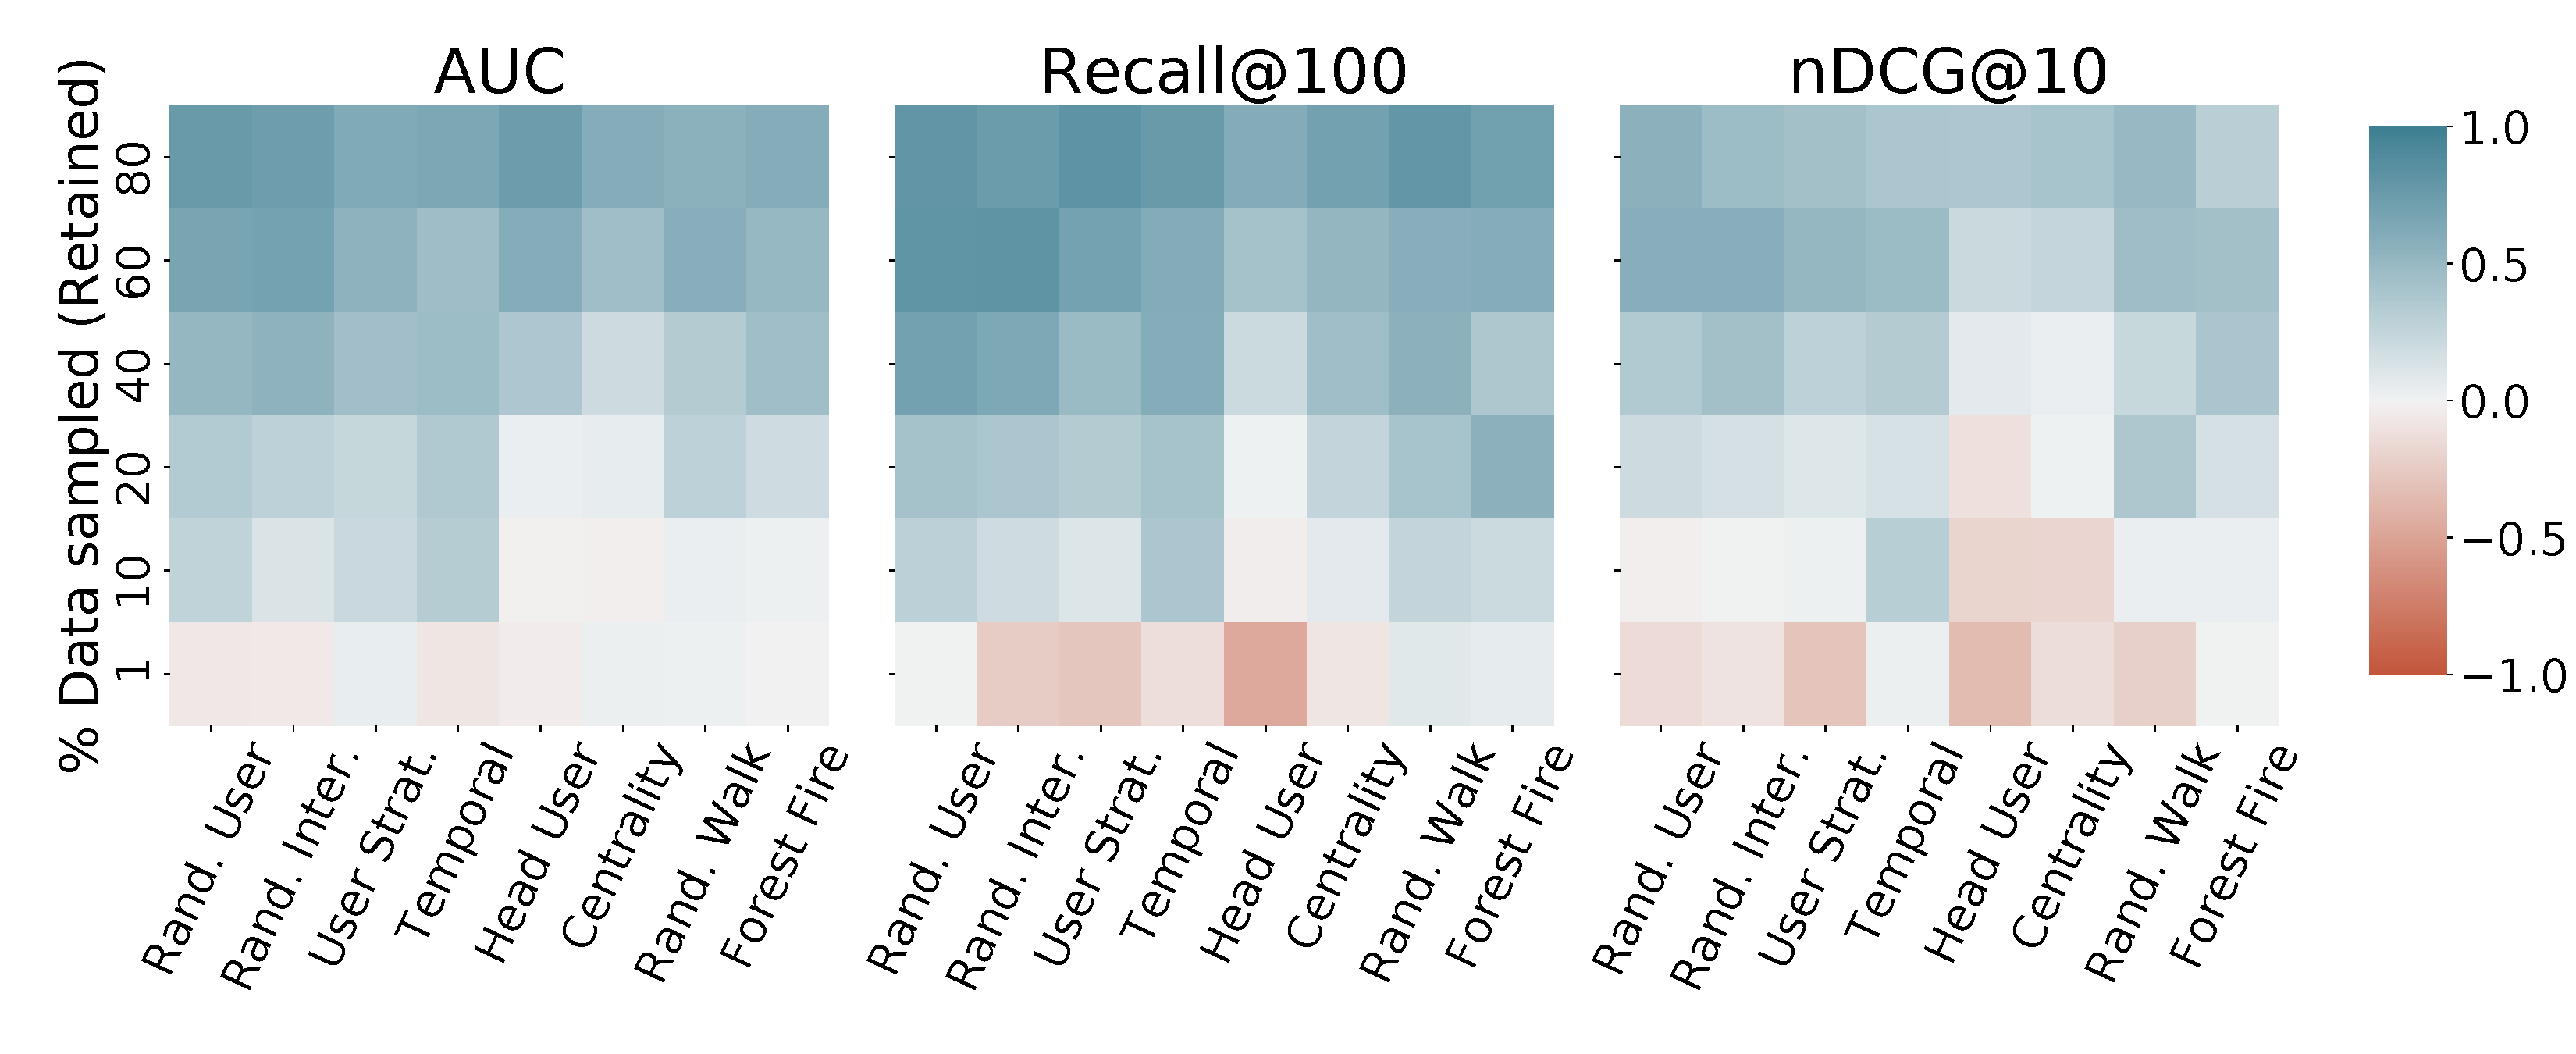
\includegraphics[width=\linewidth]{figures/percent_sampling_vs_sampler.pdf}
    \vspace{-0.8cm}
    \caption{Heatmap of the average Kendall's Tau for different samplers stratified over metrics and \% data sampled.}
    \label{metric_correlation}
    \vspace{-0.5cm}
\end{figure}
% \begin{wrapfigure}{r}{0.36\textwidth}
%     \vspace{-0.3cm}
%     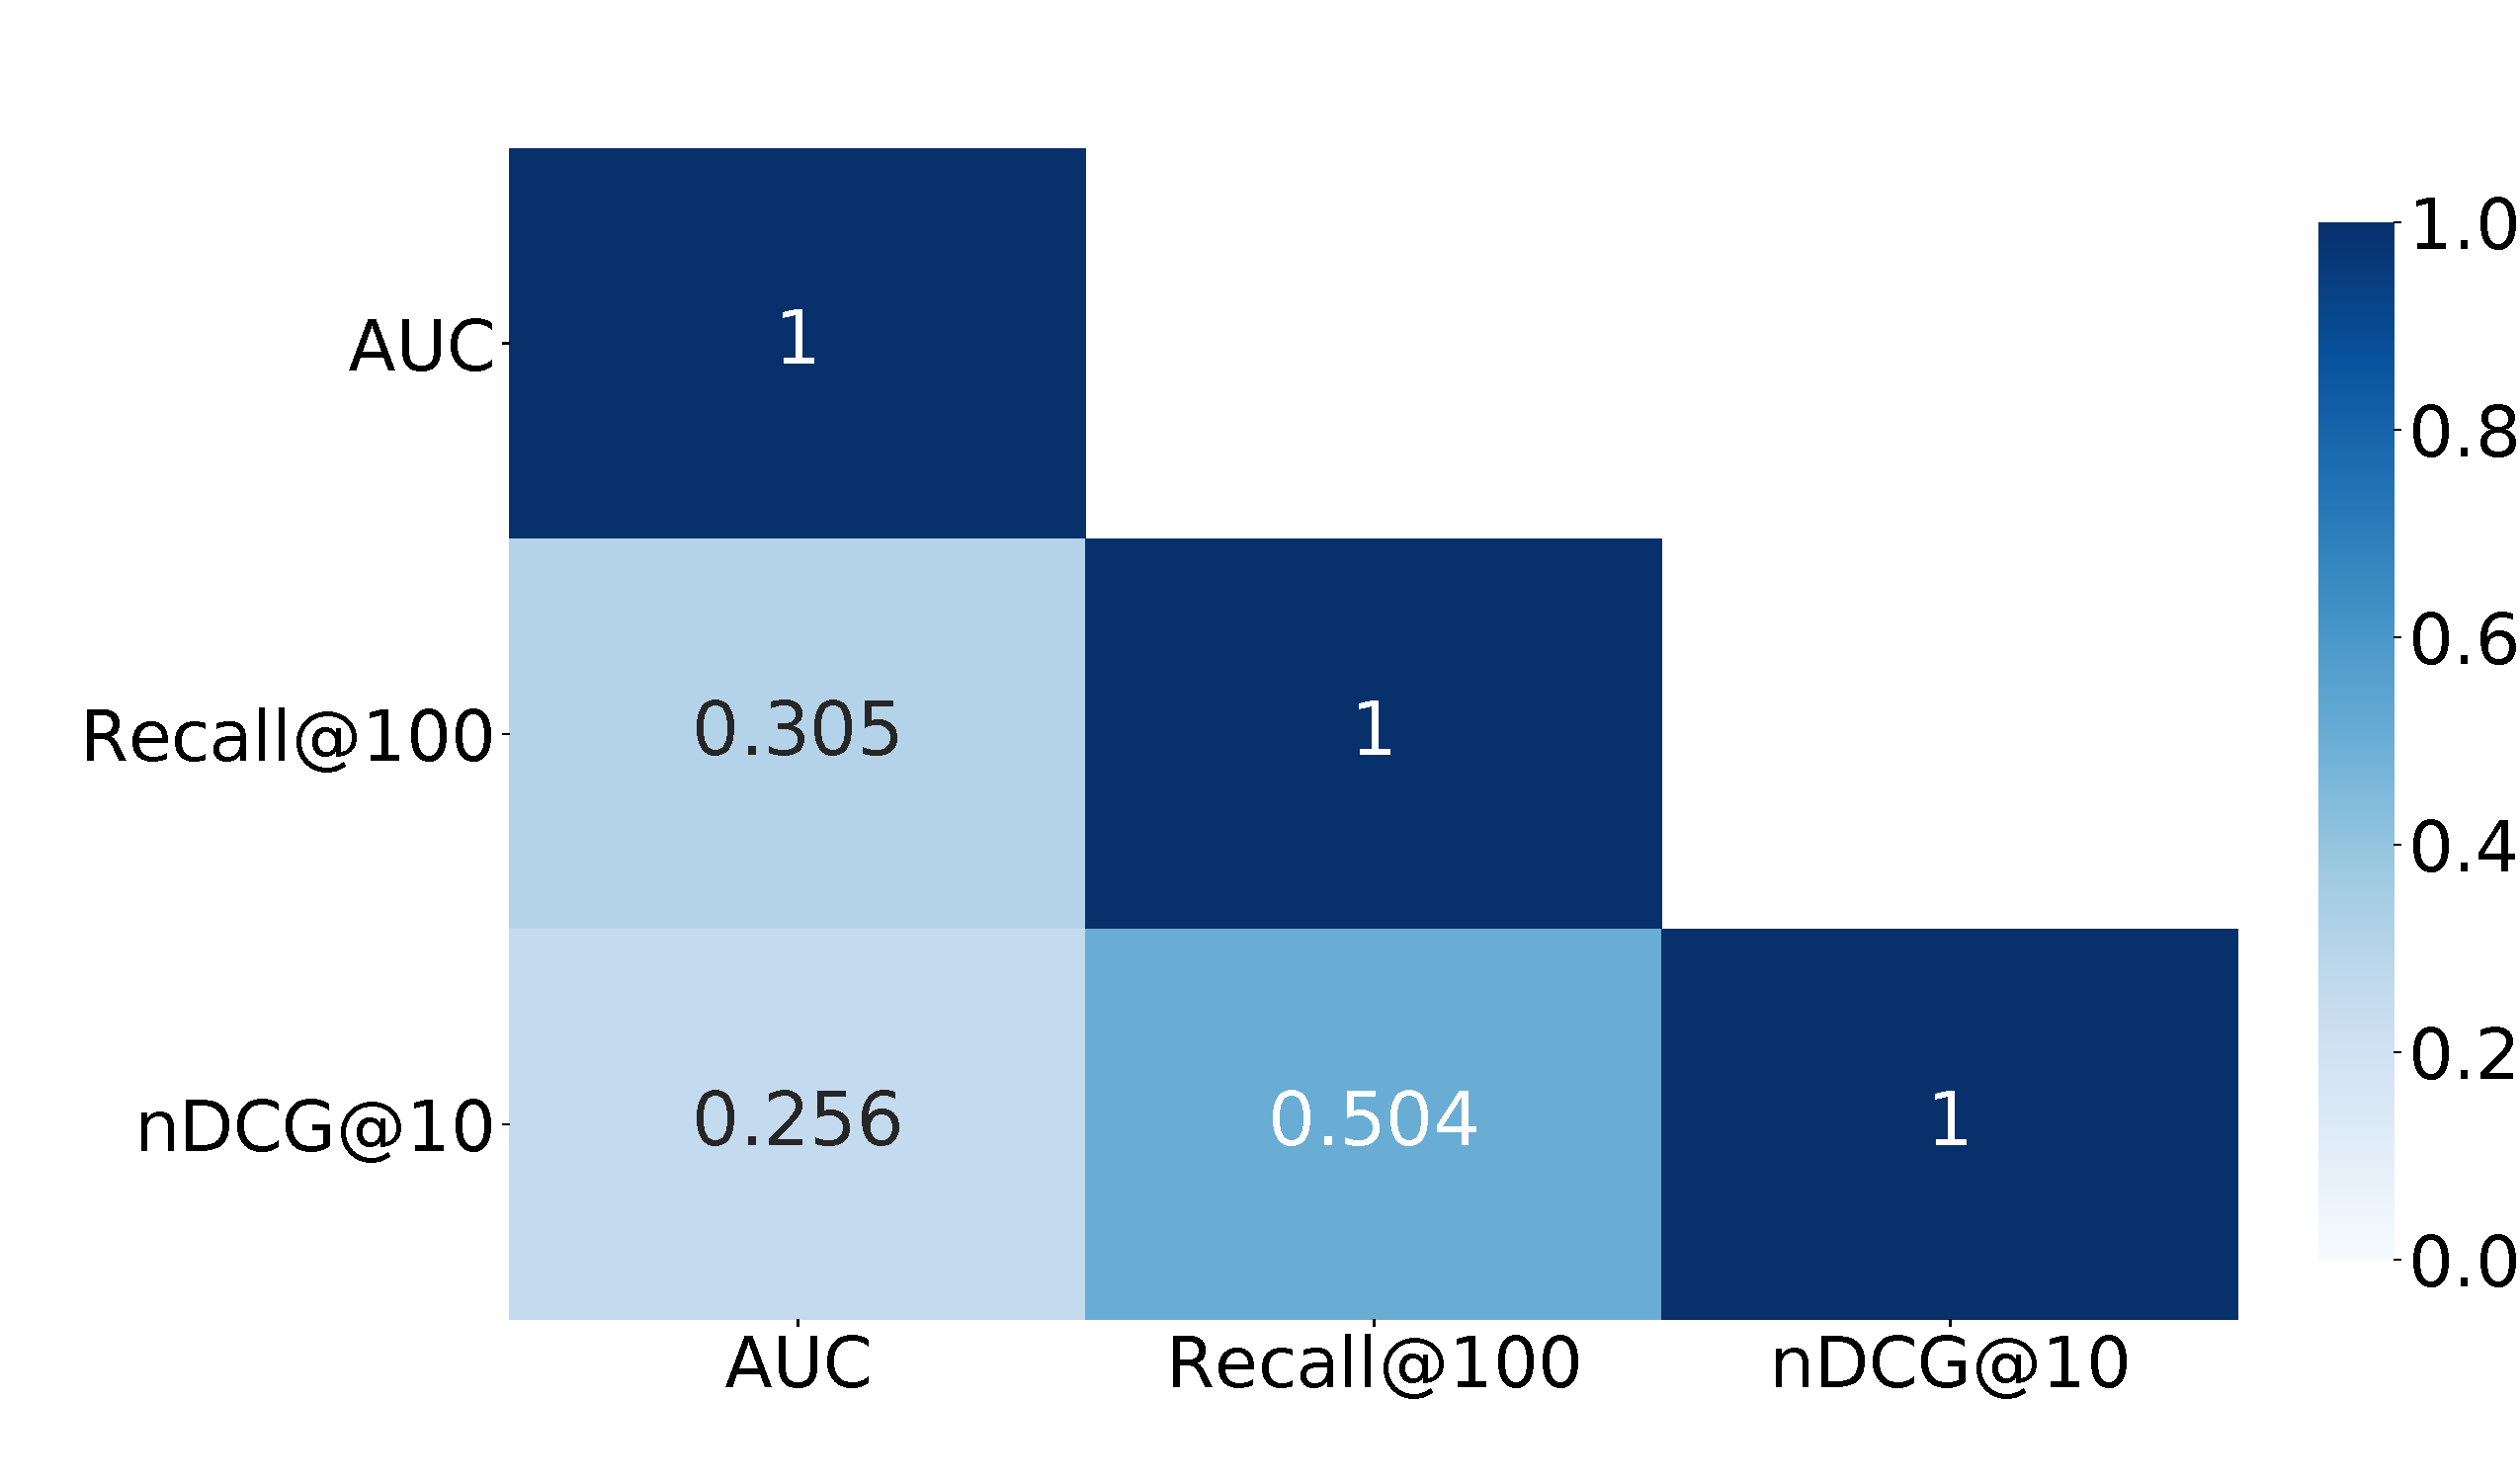
\includegraphics[width=\linewidth]{figures/metric_correlation.pdf}
%     \vspace{-0.92cm}
%     \caption{Average Kendall's Tau amongst the rankings of algorithms over different metrics.}
%     \label{metric_correlation}
%     \vspace{-0.5cm}
% \end{wrapfigure}
% \subsubsection{How do different metrics correlate with each other? \ \ } \ns{Check if we need to change this figure.} In an attempt to better understand how well do the three different implicit and sequential feedback metrics (\cref{feedback_types}) agree with each other, we visualize the average correlation between the algorithm rankings for each metric pair in \cref{metric_correlation}. To be precise, we compute the correlation between metric$_1$ and metric$_2$ as the Kendall's Tau between the ranked list of algorithms on metric$_1$ and metric$_2$ averaged over all datasets, sampling strategies and \% data sampled. We first observe that all three metrics correlate positively with each other. Finally, the AUC metric correlates less significantly with both Recall and nDCG than the correlation amongst Recall and nDCG.
\section{\oracle: Which sampler is best for me?} Although the results presented in \cref{main_exp} are indicative of correlation between the ranking of recommendation algorithms on the full dataset \vs smaller sub-samples, there still is no `one-size-fits-all' solution to the question of \emph{how to best sub-sample a dataset for retaining the performance of different recommendation algorithms?} In this section, we propose \oracle, that attempts to answer this question from a statistical perspective, in contrast with existing literature that generally has to resort to sensible heuristics \cite{large_graphs, scaling_up, sampling_cf_nn}.

\subsection{Problem formulation}
Given a dataset \dataset, we aim to gauge how a \emph{new} sampling strategy will perform in retaining the performance of different recommendation algorithms. Having already experimented with sixteen different sampling strategies on six datasets (\cref{main_exp}), we take a frequentist approach in predicting the performance of any sampling scheme. To be precise, to predict the performance of sampling scheme $s$ on dataset \dataset, we start by creating \dataset's subset according to $s$ and call it $\mathcal{D}^s$. We then represent \dataset and $\mathcal{D}^s$ in a low-dimensional latent space, followed by a powerful regression model to directly estimate the performance of $s$ on \dataset.

\subsection{Dataset representation} \label{data_rep}
We experiment with the following techniques of embedding a user-item interaction dataset into lower dimensions:

\subsubsection{Handcrafted. \ \ } For this method, we cherry-pick a few representative characteristics of \dataset and the underlying user-item bipartite interaction graph $\mathcal{G}$. Inspired by prior work \cite{large_graphs}, we represent \dataset as a combination of five features. We first utilize the frequency distribution of all users and items in \dataset. Next, we evaluate the distribution of the top$-100$ eigenvalues of $\mathcal{G}$'s adjacency matrix. All of these three distributions are generally long-tailed and heavily skewed. Furthermore, to capture notions like the diameter of $\mathcal{G}$, we compare the distribution of the number of hops $h$ \vs the number of pairs of nodes in $\mathcal{G}$ reachable at a distance less than $h$ \cite{hop_plot}. This distribution, unlike others is monotonically increasing in $h$. Finally, we also compute the size distribution of all connected components in $\mathcal{G}$, where a connected component is defined to be the maximal set of nodes, such that a path exists between any pair of nodes. Ultimately, we ascertain \dataset's final representation by concatenating $10$ evenly-spaced samples from each of the aforementioned distributions along with the total number of users, items, and interactions in \dataset. This results in a $53-$dimensional embedding for each dataset. Note that unlike previous work of simply \emph{retaining} the discussed features as a proxy of the quality of data subsets \cite{large_graphs}, \oracle instead uses these features to learn a regression model \emph{on-top} which can dynamically establish the importance of each feature in the performance of a sampling strategy.

\subsubsection{Unsupervised GCN. \ \ } With the recent advancements in the field of Graph Convolutional Networks \cite{original_gcn} to represent graph-structured data for a variety of downstream tasks, we also experiment with a GCN approach to embed $\mathcal{G}$. We modify the InfoGraph framework \cite{infograph}, which uses graph convolution encoders to obtain patch-level representations, followed by sort-pooling \cite{sort_pooling} to obtain a fixed, low-dimensional embedding for the entire graph. Since the nodes in $\mathcal{G}$ are the union of all users and items in \dataset, we randomly initialize $32-$dimensional embeddings using a Xavier-uniform prior \cite{xavier}. Parameter optimization is performed in an unsupervised fashion by maximizing the mutual information \cite{mutual_information} amongst the graph-level and patch-level representations of nodes in the same graph. We validate the best values of the latent dimension and number of layers of the GCN from $\{ 4, 8, 16, 32 \}$ and $\{ 1, 3 \}$ respectively.

\subsection{Training \& Inference} \label{oracle_architecture}
Having discussed different representation functions $\mathcal{E} : \mathcal{D} \mapsto \mathbb{R}^d$ to embed a CF-dataset in \cref{data_rep}, we now discuss \oracle's training framework agnostic to the actual details about $\mathcal{E}$. 

\paragraph{Optimization problem.} As a proxy of the performance of a sampler on a given dataset, we re-use the Kendall's Tau for each CF-scenario, metric, and sampling percent used while computing the $\Psi(\mathcal{D}, s)$ in \cref{main_exp}. To be specific, given $\mathcal{D}_{f}^{s, p}$ which is a $p\%$ sample of $f-$type feedback data $\mathcal{D}_f$, sampled according to sampling strategy $s$, we aim to estimate $\tau(\mathcal{R}_{f, m}, \mathcal{R}_{f, m}^{s, p})$ without ever computing the actual ranking of algorithms 
% $\mathcal{R}_{f, m}, \mathcal{R}_{f, m}^{s, p}$ 
on either the full or sampled datasets:
\begin{equation} \label{tau_hat}
    \hat{\tau}\left(\mathcal{R}_{f, m}, \mathcal{R}_{f, m}^{s, p}\right) = \Phi\left(\mathcal{E}(\mathcal{D}_f), \mathcal{E}(\mathcal{D}_f^{s, p}), m\right),
\end{equation}
where $\Phi$ is an arbitrary neural network, and $m$ is the metric of interest (see \cref{model_scenario_table}). We train $\Phi$ by either (1) regressing on the Kendall's Tau computed for each CF scenario, metric, and sampling percent used while computing the $\Psi(\mathcal{D}, s)$ scores in \cref{main_exp}; or (2) performing BPR-style \cite{bpr} pairwise ranking on two sampling schemes $s_i \succ s_j \iff \tau(\mathcal{R}_{f, m}, \mathcal{R}_{f, m}^{s_i, p}) > \tau(\mathcal{R}_{f, m}, \mathcal{R}_{f, m}^{s_j, p})$. Formally, the two optimization problems are defined as follows:
\begin{align*}
    \argmin{\Phi} & \sum_{\mathcal{D}_f} \sum_{s} \sum_{p} \sum_{m} \left(\tau\left(\mathcal{R}_{f, m}, \mathcal{R}_{f, m}^{s, p}\right) - \hat{\tau}\left(\mathcal{R}_{f, m}, \mathcal{R}_{f, m}^{s, p}\right) \right)^2 \\ & \text{(\oracle-regression)} \\
    \argmin{\Phi} & \sum_{\mathcal{D}_f} \sum_{s_i \succ s_j} \sum_{p} \sum_{m} -\text{ln}~\sigma\left(\hat{\tau}\left(\mathcal{R}_{f, m}, \mathcal{R}_{f, m}^{s_i, p}\right) - \hat{\tau}\left(\mathcal{R}_{f, m}, \mathcal{R}_{f, m}^{s_j, p}\right) \right) \\ & \text{(\oracle-ranking)} \\
    \text{where, \;} & \hat{\tau}\left(\mathcal{R}_{f, m}, \mathcal{R}_{f, m}^{s, p}\right) ~=~ \Phi\left(\mathcal{E}(\mathcal{D}_f), \mathcal{E}(\mathcal{D}_f^{s, p}), m\right).
\end{align*}
The critical differences between the two aforementioned optimization problems are the downstream use-case and $\Phi$'s training time. If the utility of \oracle is to rank different sampling schemes for a given dataset, then \oracle-ranking is better suited as it is robust to the noise in computing $\tau(\mathcal{R}_{f, m}, \mathcal{R}_{f, m}^{s_i, p})$ like improper hyper-parameter tuning, local minima, \etc On the other hand, \oracle-regression is better suited for the use-case of estimating the exact values of $\tau$ for a sampling scheme on a given dataset. Even though both optimization problems converge in less than $2$ minutes given the data collected in \cref{main_exp}, the complexity of optimizing \oracle-ranking is still squared \wrt the total number of sampling schemes, whilst that of \oracle-regression is linear.

\paragraph{Architecture.} To compute $\Phi(\mathcal{E}(\mathcal{D}_f), \mathcal{E}(\mathcal{D}_f^{s, p}), m)$ we concatenate $\mathcal{E}(\mathcal{D}_f)$, $\mathcal{E}(\mathcal{D}_f^{s, p})$, one-hot embedding of $m$; and pass it through two relu-activated MLP projections to obtain $\hat{\tau}(\mathcal{R}_{f, m}, \mathcal{R}_{f, m}^{s, p})$. For \oracle-regression, we also pass the final output through a tanh activation, to reflect the range of Kendall's Tau \ie $[-1, 1]$.

\paragraph{Inference.} Since computing both $\mathcal{E}$ and $\Phi$ are agnostic to the datasets and the sampling schemes, we can simply use the trained $\mathcal{E}$ and $\Phi$ functions to rank \emph{any} sampling scheme for \emph{any} CF dataset. Computationally, given a trained \oracle, the utility of a sampling scheme can be computed simply by computing $\mathcal{E}$ twice, along with a single pass over $\Phi$, completing in the order of milliseconds.

\begin{figure*} \centering
\begin{minipage}{0.47\textwidth}
    \centering
    \captionsetup{type=table} %% tell latex to change to table
    % \begin{table}[!ht]
    % \vspace{0.05cm}
    \begin{footnotesize} % normalsize, small, footnotesize
    \begin{center}
        \begin{tabular}{c c | c c c}
            \toprule
            $\mathcal{E}$ & $\Phi$ & \textbf{MSE} & \textbf{P@1} \\ \midrule
            
            \multicolumn{2}{c|}{Random} & 0.2336 & 25.2 \\ 
            \multicolumn{2}{c|}{User sampling \emph{w/} Bias-only \samplerprop} & -- & 30.6 \\ \midrule
            
            Handcrafted & Least squares regression & 0.1866 & 31.7 \\
            '' & XGBoost regression & 0.1163 & 43.9 \\
            '' & \oracle-regression & \underline{0.1008} & 51.2 \\ 
            '' & \oracle-ranking    & -- & 51.2 \\ \midrule
            
            Unsupervised GCN & Least squares regression & 0.1838 & 39.1 \\
            '' & XGBoost regression & 0.1231 & 43.9 \\
            '' & \oracle-regression & 0.1293 & 48.8 \\ 
            '' & \oracle-ranking    & -- & \underline{53.7} \\ \bottomrule
        \end{tabular}
    \end{center}
    \end{footnotesize}
    \vspace{0.5cm}
    \caption{Results for predicting the best sampling scheme for a particular dataset over a germane metric. The MSE-value next to randomly choosing the sampling scheme represents the variance of the test-set. Best values are \underline{underlined}.}
    \label{oracle_results}
    \vspace{-6mm} %Put here to reduce too much white space after your table
% \end{table}
\end{minipage} \hspace{0.8cm} %\hfill
\begin{minipage}{0.46\textwidth}
    \centering
    \vspace{-0.5cm}
    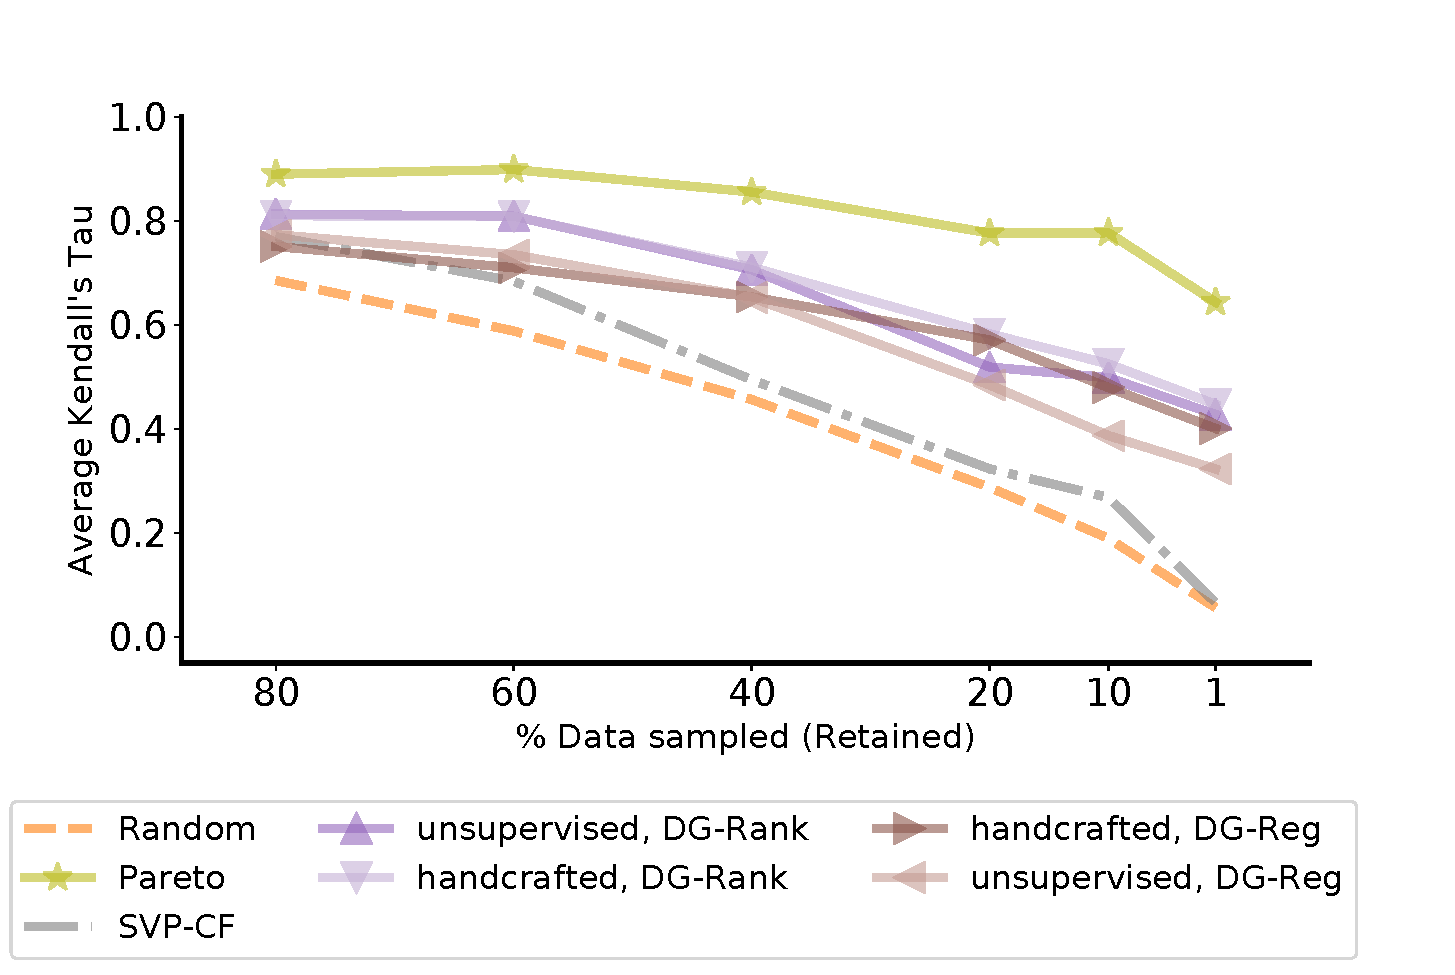
\includegraphics[width=0.86\linewidth]{figures/oracle_tau_vs_sampling_percent.pdf}
    \vspace{-0.1cm}
    \caption{Comparison of the average Kendall's Tau with \% data sampled for different sampling-selection strategies. A higher Tau indicates better retaining power of the ranking of different recommendation algorithms.}
    \label{percent_sampling_vs_tau_oracle}
\end{minipage}
\end{figure*} 

\subsection{Experiments}
\paragraph{Setup.} 
% We re-use the datasets, CF-scenarios, sampling strategies, and percentage sampling choices from \cref{main_exp}. To evaluate the competence of \oracle, we chose to perform the following train, validation, and test split: for each dataset and CF-scenario, we randomly split the metric and sampling percent $(m, p)$ join into $70/15/15\%$ proportions. Finally, during validation/testing, having fixed a dataset, CF-scenario, metric, and \% sampled data---we ask \oracle to predict the best sampler for this particular dataset. Given that there are only $16$ samplers in our study, we use the P$@1$ metric on the ranked list of samplers to evaluate \oracle.
We first create a train/validation/test split by randomly splitting all possible metrics and sampling $\%$ pairs $(m, p)$ into $70/15/15\%$ proportions. Subsequently for each dataset \dataset, CF-scenario $f$, and $(m, p)$ in the validation/test-set, we ask \oracle to rank all $16$ samplers (\cref{psi_results}) for $p\%$ sampling of $f-$type feedback for \dataset and use metric $m$ for evaluation by sorting $\hat{\tau}$ for each sampler, as defined in \cref{tau_hat}. To evaluate \oracle, we use the P$@1$ metric between the actual sampler ranking computed while computing $\Psi-$scores in \cref{main_exp}, and the one estimated by \oracle.
% Having already computed the true ranking of sampling strategies while computing $\Psi-$scores in \cref{main_exp}, we use the P$@1$ metric between the actual sampler ranking and the one estimated by sorting $\hat{\tau}$ for each sampler, as defined in \cref{tau_hat} to evaluate \oracle.

\subsubsection{How accurately can \oracle predict the best sampling scheme? \ \ } In \cref{oracle_results}, we compare all dataset representation choices $\mathcal{E}$, and multiple $\Phi$ architectures for the task of predicting the best sampling strategy. In addition to the regression and ranking architectures discussed in \cref{oracle_architecture}, we also compare with linear least-squares regression and XGBoost regression \cite{xgboost} as other choices of $\Phi$. In addition, we compare \oracle with simple baselines: (1) randomly choosing a sampling strategy; and (2) the best possible static sampler choosing strategy---always predict user sampling \emph{w/} Bias-only \samplerprop. First and foremost, irrespective of the $\mathcal{E}$ and $\Phi$ choices, \oracle outperforms both baselines. Next, both the handcrafted features and the unsupervised GCN features perform quite well in predicting the best sampling strategy, indicating that the graph characteristics are well correlated with the final performance of a sampling strategy. Finally, \oracle-regression and \oracle-ranking both perform better than alternative $\Phi-$choices, especially for the P$@1$ metric. 

% % \begin{table}[!ht]
    % \vspace{0.05cm}
    \begin{footnotesize} % normalsize, small, footnotesize
    \begin{center}
        \begin{tabular}{c c | c c c}
            \toprule
            $\mathcal{E}$ & $\Phi$ & \textbf{MSE} & \textbf{P@1} \\ \midrule
            
            \multicolumn{2}{c|}{Random} & 0.2336 & 25.2 \\ 
            \multicolumn{2}{c|}{User sampling \emph{w/} Bias-only \samplerprop} & -- & 30.6 \\ \midrule
            
            Handcrafted & Least squares regression & 0.1866 & 31.7 \\
            '' & XGBoost regression & 0.1163 & 43.9 \\
            '' & \oracle-regression & \underline{0.1008} & 51.2 \\ 
            '' & \oracle-ranking    & -- & 51.2 \\ \midrule
            
            Unsupervised GCN & Least squares regression & 0.1838 & 39.1 \\
            '' & XGBoost regression & 0.1231 & 43.9 \\
            '' & \oracle-regression & 0.1293 & 48.8 \\ 
            '' & \oracle-ranking    & -- & \underline{53.7} \\ \bottomrule
        \end{tabular}
    \end{center}
    \end{footnotesize}
    \vspace{0.5cm}
    \caption{Results for predicting the best sampling scheme for a particular dataset over a germane metric. The MSE-value next to randomly choosing the sampling scheme represents the variance of the test-set. Best values are \underline{underlined}.}
    \label{oracle_results}
    \vspace{-6mm} %Put here to reduce too much white space after your table
% \end{table}
% \begin{figure}[ht!] 
%     \centering
%     \vspace{-0.12cm}
%     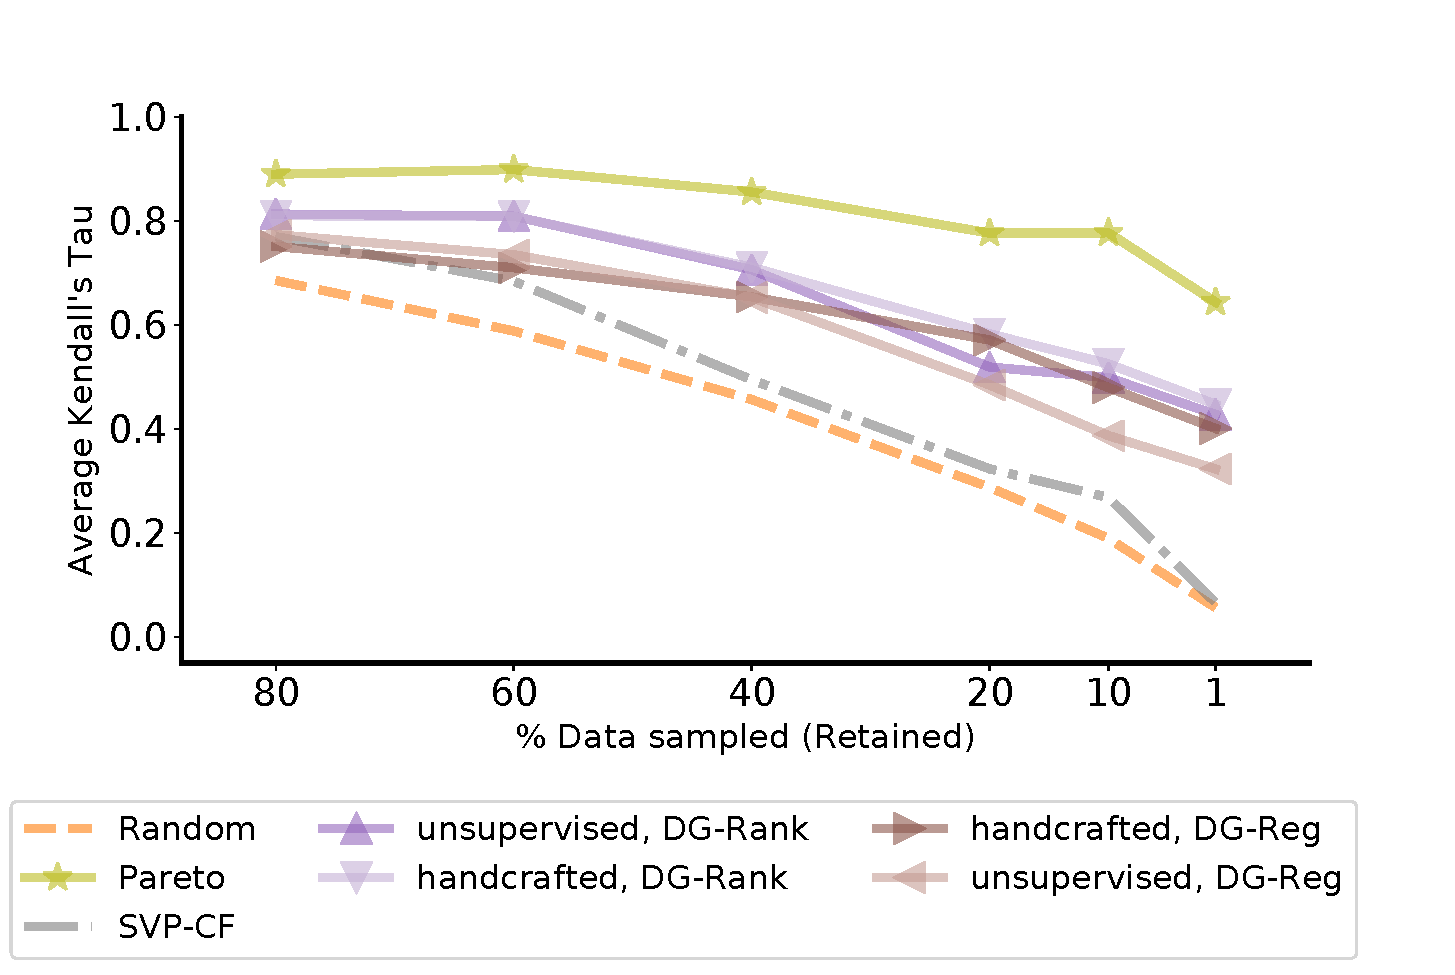
\includegraphics[width=\linewidth]{figures/oracle_tau_vs_sampling_percent.pdf}
%     \vspace{-0.5cm}
%     \caption{Comparison of the average Kendall's Tau with \% data sampled for different sampling-selection strategies. A higher Tau indicates better retaining power of the ranking of different recommendation algorithms.}
%     \label{percent_sampling_vs_tau_oracle}
% \end{figure} 

\subsubsection{Can we use \oracle to sample more data without compromising performance? \ \ } In \cref{percent_sampling_vs_tau_oracle}, we compare the impact of \oracle in sampling more data by dynamically choosing an appropriate sampler for a given dataset, metric, and $\%$ data to sample. 
% As a real-world benchmark for performance of \oracle, 
More specifically,
we compare the percentage of data sampled with the Kendall's Tau averaged over all datasets, CF-scenarios, and relevant metrics for different sampling strategy selection approaches. We compare \oracle with: (1) randomly picking a sampling strategy averaged over $100$ runs; and (2) the Pareto frontier as a skyline which always selects the best sampling strategy for any CF-dataset. As we observe from \cref{percent_sampling_vs_tau_oracle}, \oracle is better than predicting a sampling scheme at random, and 
% pushes the average Kendall's Tau
is
much closer to the Pareto frontier. Next, pairwise ranking approaches are marginally better than regression approaches 
% for both the handcrafted and unsupervised-GCN data features.
irrespective of $\mathcal{E}$. Finally, \oracle can appraise the best-performing recommendation algorithm with a suitable amount of confidence using only $10\%$ of the original data. This is significantly more efficient compared to having to sample $50-60\%$ if we were to always sample using a fixed strategy.
% \section{Conclusion} 
\section{Conclusion}
\label{sec_conclusions}

Our work consists of two studies that quantitatively and qualitatively investigate the influence of a CI service (e.g., \textsc{TravisCI}), and CI as a practice, on the time-to-delivery of merged PRs, respectively. In our quantitative study, we analyze 162,653 PRs of 87 GitHub projects to understand the factors that influence (and improve) the delivery time of merged PRs. In our qualitative study, we analyze 450 survey responses from participants of 73 projects (out of the initial 87 projects). We investigate the perceived influence of CI on the delivery time of merged PRs. We also study the perceived influence of CI on the code review and release processes.

As a key takeaway, our studies demonstrate that the adoption of \textsc{TravisCI}
will not necessarily deliver or merge PRs more quickly. Instead, the pivotal benefit of a CI service is to improve the mechanisms by which contributions to projects are processed (e.g., facilitating decisions on PR submissions), without compromising the quality of the project or overloading developers. The automation provided by CI and the boost in developers' confidence are key aspects of using CI. For instance, CI may help the process of sorting which PRs are worth reviewing (e.g., PRs with green builds).
Furthermore, open-source projects wishing to attract and retain external contributors should consider the use of CI in their pipeline, since CI is perceived to lower the contribution barrier while making contributors feel more confident and engaged in the project.

\section*{Acknowledgments}
\label{sec_Acknowledgments}

This work is partially supported by INES (\url{www.ines.org.br}), CNPq grants 465614/2014-0 and 425211/2018-5, CAPES grant 88887.136410/2017-00, FACEPE grants APQ-0399-1.03/17, and PRONEX APQ/0388-1.03/14.

\section*{Data Availability}
For replication purposes, we publicize our datasets and results to the interested researcher: \url{https://prdeliverydelay.github.io/#datasets}

\section*{Declarations}

\textbf{Conflict of interests}. The authors declare that they have no conflict of interest.
\section{Discussion} \section{Discussion}
\label{ss: discussion}

In this section, we discuss how security scanners can defend against evasions (Section~\ref{ss:anti-evasion})
and what limitations our work currently has (Section~\ref{ss:extension}).

\subsection{Mitigating Evasions}
\label{ss:anti-evasion}

One way to mitigate dynamic evasions is to adapt general anti-evasion techniques from other domains to the problem of analyzing PDF documents.
Several recent papers propose to load a potentially malicious file in environments targeted at revealing the malicious behavior of the file.
For example, FuzzDroid~\cite{rasthofer2017making}, IntelliDroid~\cite{wong2016intellidroid}, and SmartDroid~\cite{zheng2012smartdroid} try to cause a potentially malicious Android app to reach ``sensitive'' API calls that would reveal malicious behavior, such as sending an SMS to a premium number.
Adapting this technique to PDF scanners requires identifying sensitive APIs in PDFs.
For known exploits, such APIs may be known, e.g., it is known that the ``Toolbutton'' exploit relies on calling the \code{app.addToolButton} API.
Finding sensitive APIs for previously unknown exploits remains an open research problem.
A related technique to cope with dynamic evasions is to explore multiple execution paths for branch decisions that depend on the environment in which a file is executed.
Rozzle~\cite{rozzle-de-cloaking-internet-malware-2} proposes this idea for client-side JavaScript code.
Adapting their approach is a promising direction for mitigating the environment-related dynamic evasions.

To deal with UI-related evasions, dynamic scanners could adapt ideas used in PuppetDroid~\cite{gianazza2014puppetdroid} and PyTrigger~\cite{fleck2013pytrigger}.
These approaches record an interaction trace from a human and play it back when loading the file under analysis to get through possible checks that guard the attack.
One of the dynamic scanners studied in this work, Cuckoo, mitigates evasions using a simpler form of this idea: The scanner arbitrarily moves the mouse to simulate a human user~\cite{cuckoo_mouse_movement}.
However, this mitigation technique is unlikely to work for evasions that require a more complicated user interaction, such as a ``captcha''.

To identify files that behave differently in an analysis environment, some techniques compare the execution behavior of the file in several different environments, e.g. virtual and physical~\cite{balzarotti2010efficient}.
Another kind of anti-evasion technique is to hide any difference between a virtual and a physical execution environment to fool the evasive malware~\cite{shi2018handling}.
%
Finally, to deal with the large number of possible evasions and combinations of evasions, training machine learning models to distinguish benign from malicious files seems to be a worthwhile direction~\cite{smutz2012malicious,vsrndic2013detection,laskov2011static,corona2014lux0r}.
The main challenge for effectively training machine learning models is to obtain a sufficiently large set of labeled data.
Our framework could serve as a generator of malicious training files that use different evasions and combinations of evasions.

The high recall of SAFE-PDF~\cite{2018arXiv181012490J}, which is based on abstract interpretation of JavaScript code embedded in PDFs, shows that conservative program analysis may provide an effective way of detecting malicious behavior despite evasions. The downside of any conservative program analysis are spurious warnings, which the relatively high false positive ratio of SAFE-PDF confirms.



\subsection{Choice of Scanners}
\label{ss:extension}

We focus on in-production, commercial security scanners because they represent the current state-of-the-practice, and recent academic scanners because they represent the state-of-the-art.
The studied scanners contain more static than dynamic scanners because static scanners currently dominate the market.
For example, the VirusTotal service aggregates more than 60 static scanners at the time of writing this paper~\cite{vt_engines_count}, whereas we could find only ten commercial dynamic scanners, out of which three consented to participate in this research.

Our work should not be understood as a comparison of different scanners, but rather as a comparison of each scanner's effectiveness before and after adding evasions.
The version of the scanners used in online aggregation services, which we use for the studied static scanners, may differ from the full-fledged scanners, because vendors may optimize the response time for an online service~\cite{pitfall}.



%%
%% The acknowledgments section is defined using the "acks" environment
%% (and NOT an unnumbered section). This ensures the proper
%% identification of the section in the article metadata, and the
%% consistent spelling of the heading.
\begin{acks}
This work was partly supported by NSF Award \#1750063.
\end{acks}

%%
%% The next two lines define the bibliography style to be used, and
%% the bibliography file.
\bibliographystyle{ACM-Reference-Format}
\bibliography{acmart}

%%
%% If your work has an appendix, this is the place to put it.
% \appendix

% \section{Research Methods}
% \subsection{Part One}
% \subsection{Part Two}

% \section{Online Resources}

\end{document}
\endinput
%%
%% End of file `sample-sigconf.tex'.

We study the practical consequences of dataset sampling strategies on the ranking performance of recommendation algorithms. Recommender systems are generally trained and evaluated on \emph{samples} of larger datasets. Samples are often taken in a na\"ive or ad-hoc fashion: \eg by sampling a dataset randomly or by selecting users or items with many interactions. As we demonstrate, commonly-used data sampling schemes can have significant consequences on algorithm performance. Following this observation, this paper makes three main contributions: (1) \emph{characterizing} the effect of sampling on algorithm performance, in terms of algorithm and dataset characteristics (\eg sparsity characteristics, sequential dynamics, \etc); (2) designing \sampler, which is a data-specific sampling strategy, that aims to preserve the relative performance of models after sampling, and is especially suited to long-tailed interaction data; and (3) developing an \emph{oracle}, \oracle, which can suggest the sampling scheme that is most likely to preserve model performance for a given dataset. The main benefit of \oracle is that it will allow recommender system practitioners to quickly prototype and compare various approaches, while remaining confident that algorithm performance will be preserved, once the algorithm is retrained and deployed on the complete data. Detailed experiments show that using \oracle, we can discard upto $5\times$ more data than any sampling strategy with the same level of performance.
\begin{table}[!ht]
    \vspace{-5mm} %Put here to reduce too much white space after your table
    \begin{footnotesize} % normalsize, small, footnotesize
    \begin{center}
        \begin{tabular}{c c}
            \toprule
            \textbf{Consumption} & \textbf{CO$_2$e (lbs.)} \\ \midrule
            
            1 person, NY$\leftrightarrow$SF flight      & 2k \\
            Human life, 1 year avg.                     & 11k \\ 
            \midrule
            Weekly RecSys development cycle             & 20k \\
            '' \ \ \ \ \emph{w/} \oracle                & 3.4k \\
            
            \bottomrule
        \end{tabular}
    \end{center}
    \end{footnotesize}
    \vspace{2mm}
    \caption{CO$_2$ emissions comparison \cite{co2e}}
    % \caption*{Table 1: CO$_2$ emissions comparison}
    \label{co2e}
    \vspace{-10mm} %Put here to reduce too much white space after your table
\end{table}
Given our motivation of quickly benchmarking recommendation algorithms, we now aim to \emph{characterize} the performance of various commonly-used sampling strategies. We loosely define the performance of a sampling scheme as 
%it's
its
ability in effectively retaining the performance-ranking of different recommendation algorithms on the full \vs sub-sampled data. In this section, we start by discussing the different recommendation feedback scenarios we consider, along with a representative sample of popular recommendation algorithms that we aim to efficiently benchmark. We then examine popular data sampling strategies, followed by proposing a novel, proxy-based sampling strategy (\sampler) that is especially suited for sampling representative subsets from long-tail CF data.

\subsection{Problem Settings \& Methods Compared} \label{feedback_types} \label{algorithms}
To give a representative sample of typical recommendation scenarios, we consider three different user feedback settings. In \emph{explicit feedback}, each user $u$ gives a numerical rating $r^u_i$ to each interacted item $i$; the model must predict these ratings for novel (test) user-item interactions. Models from this class are evaluated in terms of the Mean Squared Error (MSE) of the predicted ratings. Another scenario we consider is \emph{implicit feedback}, where the interactions for each user are only available for positive items (\eg clicks or purchases), whilst all non-interacted items are considered as negatives. We employ the AUC, Recall@$100$, and nDCG@$10$ metrics to evaluate model performance for implicit feedback algorithms. Finally, we also consider \emph{sequential feedback}, where each user $u$ interacts with an ordered sequence of items $\mathcal{S}^u = (\mathcal{S}^u_1, \mathcal{S}^u_2, \ldots, \mathcal{S}^u_{|\mathcal{S}^u|})$ such that $\mathcal{S}^u_i \in \mathcal{I}$ for all $i \in \{1, \ldots, |\mathcal{S}^u|\}$. Given $\mathcal{S} = \{ \mathcal{S}^u ~|~ \forall u \in \mathcal{U} \}$, the goal is to identify the \emph{next-item} for each sequence $\mathcal{S}^u$ that each user $u$ is most likely to interact with. We use the same metrics as in implicit feedback settings. Note that following recent warnings against sampled metrics for evaluating recommendation algorithms \cite{sampled_metrics, castells_sampling}, we compute both Recall and nDCG by ranking \emph{all} items in the dataset. Further specifics about the datasets used, pre-processing, train/test splits, \etc are discussed in-depth in \cref{main_exp}. 

Given the diversity of the scenarios discussed above, there are numerous relevant recommendation algorithms. We use the following seven recommendation algorithms, intended to represent the state-of-the-art and standard baselines:
\begin{itemize}
    \listheader{PopRec:} A na\"ive baseline that simply ranks items according to overall train-set popularity. Note that this method is unaffected by the user for which items are being recommended, and has the \emph{same global ranking} of all items.
    
    \listheader{Bias-only:} Another simple baseline that assumes no interactions between users and items. Formally, it learns: (1) a global bias $\alpha$; (2) scalar biases $\beta_u$ for each user $u \in \mathcal{U}$; and (3) scalar biases $\beta_i$ for each item $i \in \mathcal{I}$. Ultimately, the rating/relevance for user $u$ and item $i$ is modeled as $\hat{r}^u_i = \alpha + \beta_u + \beta_i$.

    \listheader{Matrix Factorization (MF) \cite{mf}:} Represents both users and items in a common, low-dimensional latent-space by factorizing the user-item interaction matrix. Formally, the rating/relevance for user $u$ and item $i$ is modeled as $\hat{r}^u_i = \alpha + \beta_u + \beta_i + \gamma_u \cdot \gamma_i$ where $\gamma_u, \gamma_i \in \mathbb{R}^d$ are learned latent representations. 
    
    \listheader{Neural Matrix Factorization (NeuMF) \cite{neural_mf}:} Leverages the representation power of deep neural-networks to capture non-linear correlations between user and item embeddings. Formally, the rating/relevance for user $u$ and item $i$ is modeled as $\hat{r}^u_i = \alpha + \beta_u + \beta_i + f(\gamma_u ~||~ \gamma_i ~||~ \gamma_u \cdot \gamma_i)$ where $\gamma_u, \gamma_i \in \mathbb{R}^d$, `||' represents the concatenation operation, and $f : \mathbb{R}^{3d} \mapsto \mathbb{R}$ represents an arbitrarily complex neural network. 
    
    \listheader{Variational Auto-Encoders for Collaborative Filtering (MVAE) \cite{mvae}:} Builds upon the Variational Auto-Encoder (VAE) \cite{vae} framework to learn a low-dimensional representation of a user's consumption history. More specifically, MVAE encodes each user's bag-of-words consumption history using a VAE and further decodes the latent representation to obtain the completed user preference over all items.
    
    \listheader{Sequential Variational Auto-Encoders for Collaborative Filtering (SVAE) \cite{svae}:} A sequential algorithm that combines the temporal modeling capabilities of a GRU \cite{gru} along with the representation power of VAEs. Unlike MVAE, SVAE uses a GRU to encode the user's consumption sequence followed by a multinomial VAE at each time-step to model the likelihood of the next item. 
    
    \listheader{Self-attentive Sequential Recommendation (SASRec) \cite{sasrec}:} Another sequential algorithm that relies on the sequence modeling capabilities of self-attentive neural networks \cite{self_attention} to predict the occurance of the 
    %next-item 
    next item
    in a user's consumption sequence. To be precise, given a user $u$ and 
    %it's
    their
    time-ordered consumption history  $\mathcal{S}^u = (\mathcal{S}^u_1, \mathcal{S}^u_2, \ldots, \mathcal{S}^u_{|\mathcal{S}^u|})$, SASRec first applies self-attention on $\mathcal{S}^u$ followed by a series of non-linear feed-forward layers to finally obtain the next item likelihood.
\end{itemize}
We also list 
%the pertinence of 
models and metrics for each of the three different CF-scenarios in \cref{model_scenario_table}. Since bias-only, MF, and NeuMF can be trained for all three CF-scenarios, we optimize them using the regularized least-squares regression loss for explicit feedback, and the pairwise-ranking (BPR \cite{bpr}) loss for implicit/sequential feedback. Note however that the aforementioned algorithms are only intended to be a representative sample of a 
%wide-pool 
wide pool
of recommendation algorithms, and in our pursuit to benchmark recommender systems faster, we are primarily concerned with the \emph{ranking} of different algorithms on the full dataset \vs a smaller sub-sample.

\begin{table*}[!ht]
    \begin{small} % normalsize, small, footnotesize
    \begin{center}
        % \begin{subtable}{0.5\linewidth}
        % \centering
        %     \begin{tabular}{c | c c c}
        %         \toprule
        %         \multirow{2}{*}{Algorithm} & \multicolumn{3}{c}{CF-scenario} \\
        %         & Explicit & Implicit & Sequential \\ \midrule
                
        %         Bias-only   & Yes & Yes & Yes \\
        %         MF          & Yes & Yes & Yes \\
        %         NeuMF       & Yes & Yes & Yes \\
        %         PopRec      & $\times$ & Yes & Yes \\
        %         MVAE        & $\times$ & Yes & Yes \\
        %         SVAE        & $\times$ & $\times$ & Yes \\
        %         SASRec      & $\times$ & $\times$ & Yes \\ \bottomrule
        %     \end{tabular}
        % \end{subtable}%
        % \begin{subtable}{0.5\linewidth}
        % \centering
        %     \begin{tabular}{c | c c c}
        %         \toprule
        %         \multirow{2}{*}{Metric} & \multicolumn{3}{c}{CF-scenario} \\
        %         & Explicit & Implicit & Sequential \\ \midrule
                
        %         MSE       & Yes & $\times$ & $\times$ \\
        %         AUC       & $\times$ & Yes & Yes \\
        %         Recall@k  & $\times$ & Yes & Yes \\
        %         nDCG@k    & $\times$ & Yes & Yes \\ \bottomrule
        %     \end{tabular}
        % \end{subtable}%
        \begin{tabular}{c | c c c c c c c | c c c c}
            \toprule
            \multirow{3}{*}{CF-scenario} & \multicolumn{7}{c|}{\emph{Algorithm}} & \multicolumn{4}{c}{\emph{Metric}} \\
            & \multicolumn{7}{c|}{} & \multicolumn{4}{c}{} \\
            & Bias-only & MF & NeuMF & PopRec & MVAE & SVAE & SASRec & MSE & AUC & Recall@k & nDCG@k \\ \midrule
            Explicit & Yes & Yes & Yes & $\times$ & $\times$ & $\times$ & $\times$ & Yes & $\times$ & $\times$ & $\times$ \\[0.6mm]
            Implicit & Yes & Yes & Yes & Yes & Yes & $\times$ & $\times$ & $\times$ & Yes & Yes & Yes \\[0.6mm]
            Sequential & Yes & Yes & Yes & Yes & Yes & Yes & Yes & $\times$ & Yes & Yes & Yes \\[0.6mm]
            \bottomrule
        \end{tabular}
    \end{center}
    \end{small}
    \bigskip
    \caption{Demonstrates the pertinence of each CF-scenario towards each algorithm (left) and each metric (right). Note that we can use ranking metrics for explicit feedback, however, we only use MSE as a design choice and due to it's direct relevance.}
    \label{model_scenario_table}
    \vspace{-6mm} %Put here to reduce too much white space after your table
\end{table*}

\subsection{Sampling Strategies} \label{common_sampling_schemes}
Given a user-item CF dataset \dataset, we aim to create a $p\%$ subset $\mathcal{D}^{s, p}$ according to some sampling strategy $s$. In this paper, to be comprehensive, we consider a sample of eight popular sampling strategies, which can be grouped into the following three categories:

\subsubsection{Interaction sampling. \ \ } We first discuss three strategies that sample interactions from \dataset. In \emph{Random Interaction Sampling}, we generate $\mathcal{D}^{s, p}$ by randomly sampling $p\%$ of all the user-item interactions in \dataset. \emph{User-history Stratified Sampling} is another popular sampling technique (see \eg \cite{svae, handbook}) to generate smaller CF-datasets. To match the user-frequency distribution amongst \dataset and $\mathcal{D}^{s, p}$, it randomly samples $p\%$ of interactions from each user's consumption history. Unlike random stratified sampling, \emph{User-history Temporal Sampling} samples $p\%$ of the \emph{most recent} interactions for each user. This strategy is representative of the popular practice of making data subsets from the online traffic of the last $x$ days \cite{eclare, pfastre}.

\subsubsection{User sampling. \ \ } Similar to sampling interactions, we also consider two strategies which sample users in \dataset instead. To ensure a fair comparison amongst the different kinds of sampling schemes used in this paper, we retain exactly $p\%$ of the \emph{total interactions} in $\mathcal{D}^{s, p}$. In \emph{Random User Sampling}, we retain users from \dataset at random. To be more specific, we iteratively preserve \emph{all} the interactions for a random user until we have retained $p\%$ of the original interactions. Another strategy we employ is \emph{Head User Sampling}, in which we iteratively remove the user with the least amount of total interactions. This method is representative of commonly used data pre-processing strategies (see \eg \cite{mvae, neural_mf}) to make data suitable for parameter-heavy algorithms. Sampling the data in such a way can introduce bias toward users from minority groups which might raise concerns from a diversity and fairness perspective \cite{fairness}.

\subsubsection{Graph sampling. \ \ } Instead of sampling directly from \dataset, we also consider three strategies that sample from the inherent user-item bipartite interaction graph $\mathcal{G}$. In \emph{Centrality-based Sampling}, we proceed by computing the pagerank centrality scores \cite{pagerank} for each node in $\mathcal{G}$, and retain all the edges (interactions) of the \emph{top scoring nodes} until a total $p\%$ of the original interactions have been preserved. Another popular strategy we employ is \emph{Random-walk Sampling} \cite{large_graphs}, which performs multiple random-walks with restart on $\mathcal{G}$ and retains the edges amongst those pairs of nodes that have been visited at least once. We keep expanding our walk until $p\%$ of the initial edges have been retained. We also utilize \emph{Forest-fire Sampling} \cite{forest_fire}, which is a snowball sampling method and proceeds by randomly ``burning'' the outgoing edges of visited nodes. It initially starts with a random node, and then propagates to a random subset of previously unvisited neighbors. The propagation is terminated once we have created a graph-subset with $p\%$ of the initial edges.

\subsection{\sampler: Selection-Via-Proxy for CF data} \label{svp_cf} 
Selection-Via-Proxy (SVP) \cite{svp} is a leading coreset mining technique for classification datasets like CIFAR10 \cite{cifar} and ImageNet \cite{image_net}. The main idea proposed is simple and effective, and proceeds by training a relatively inexpensive base-model as a proxy to define the ``importance'' of a data-point. However, applying SVP to CF-data can be highly non-trivial because of the following impediments:
\begin{itemize}
    \listheader{Data heterogeneity:} Unlike classification data 
    % $\mathcal{D}_c = \left\{ (x, y) ~|~ x \in \mathbb{R}^d, y\in \mathcal{Y}\right\}$ 
    over some input space $\mathcal{X}$ and label-space $\mathcal{Y}$, CF-data consists of numerous four-tuples $\{u, i, r^u_i, t^u_i\}$. Such multimodal data adds many different dimensions to sample data from, making it increasingly complex to define meaningful samplers. 
    
    \listheader{Defining the importance of a data point:} Unlike classification, where we can measure the performance of a classifier by 
    %it's
    its
    empirical risk on held-out data, for recommendation, there are a variety of different scenarios (\cref{feedback_types}) along with a wide list of relevant evaluation metrics. Hence, it becomes challenging to adapt importance-tagging techniques like greedy k-centers \cite{k_centers}, forgetting-events \cite{forgetting_events}, \etc for recommendation tasks.
    
    \listheader{Missing data:} 
    CF-data is well-known for (1) 
    %it's 
    its
    sparsity; (2) skewed and long-tail user/item distributions; and (3) missing-not-at-random (MNAR) properties of the user-item interaction matrix. This results in additional problems as we are now sampling data from skewed, MNAR data, especially using proxy-models trained on the same skewed data. Such sampling in the worst-case might even lead to exacerbating existing biases in the data or even aberrant data samples.
\end{itemize}
To address these fundamental limitations in applying the SVP philosophy to CF-data, we propose \sampler to sample representative subsets from large user-item interaction data. \sampler is also specifically devised for our objective of benchmarking different recommendation algorithms, as it relies on the crucial assumption that the ``easiest'' part of a dataset will generally be easy \emph{for all} algorithms. Under this assumption, even after removing such data we are still likely to retain the overall algorithms' ranking.

Because of the inherent data heterogeneity in user-item interaction data, we can sub-sample in a variety of different ways. We design \sampler to be versatile in this aspect as it can be applied to sample users, items, interactions, or combinations of them, by marginally adjusting the definition of importance of each data-point. In this paper, we limit the discussion to only sampling users and interactions (separately), but extending \sampler for sampling across other data modalities should be relatively straightforward.

Irrespective of whether to sample users or interactions, \sampler proceeds by training an inexpensive proxy model $\mathcal{P}$ on the full, original data \dataset and modifies the forgetting-events approach \cite{forgetting_events} to retain the points with the \emph{highest} importance. To be more specific, for explicit feedback, we define the importance of each data-point \ie $\{u, i, r^u_i, t^u_i\}$ interaction as $\mathcal{P}$'s average MSE (over epochs) of the specific interaction if we're sampling interactions \emph{or} $\mathcal{P}$'s average MSE of $u$ (over epochs) if we're sampling users. Whereas, for implicit and sequential feedback, we use $\mathcal{P}$'s average inverse-AUC while computing the importance of each data-point. For the sake of completeness, we experiment with both Bias-only and MF as two different kinds of proxy-models for \sampler. Since both models can be trained for all three CF-scenarios (\cref{model_scenario_table}), we can directly use them to tag the importance for each CF-scenario.

Ultimately, to handle the MNAR and long-tail problems, we also propose \samplerprop which employs user and item propensities to correct the distribution mismatch while estimating the importance of each datapoint. More specifically, let $p_{u, i} = P(r^u_i = 1 ~|~ \overstar{r}^u_i = 1)$ denote the probability of user $u$ and item $i$'s interaction actually being observed (propensity), $E$ be the total number of epochs that $\mathcal{P}$ was trained for, $\mathcal{P}_e$ denote the proxy model after the $e^{\mathit{th}}$ epoch, $\mathcal{I}_u^+ \coloneqq \{ j ~|~ r^u_j > 0 \}$ be the set of positive interactions for $u$, and $\mathcal{I}_u^- \coloneqq \{ j ~|~ r^u_j = 0 \}$ be the set of negative interactions for $u$; then, the importance function for \samplerprop, $\mathcal{I}_p$ is defined as follows:
\begin{align*}
% \begin{gathered}
    \mathcal{I}_p(u ~|~ \mathcal{P}) \coloneqq \frac{1}{|\mathcal{I}_u^+|} \cdot \sum_{i \in \mathcal{I}_u^+} \mathcal{I}_p(u, i ~|~ \mathcal{P}) \hspace{0.63em} ; \hspace{0.63em}
    \mathcal{I}_p(u, i ~|~ \mathcal{P}) \coloneqq \frac{\Delta(u, i ~|~ \mathcal{P})}{p_{u, i}} \\
    %where, 
% \end{gathered}
\end{align*}
\vspace{-0.6cm}
\begin{equation*}
\begin{gathered}
    \text{where,}
    \qquad \Delta(u, i ~|~ \mathcal{P}) \coloneqq 
    \begin{dcases} 
      ~~ \sum_{e=1}^{E} \left(\mathcal{P}_e(u, i) - r^u_i\right)^2 \\  %& \, \text{for explicit feedback} \\
      ~~ \text{(for explicit feedback)} \\ \\
      ~~ \sum_{e=1}^{E} \sum_{j \sim \mathcal{I}_u^-} \frac{1}{\mathds{1}\left(\mathcal{P}_e(u, i) > \mathcal{P}_e(u, j)\right)} \\ % & \, \text{for implicit/sequential feedback}
      ~~ \text{(for implicit/sequential feedback)}
   \end{dcases}
\end{gathered}
\end{equation*}
\vspace{0.1cm}

\begin{proposition}
Given an ideal propensity-model $p_{u, i}; \ \mathcal{I}_p(u, i ~|~ \mathcal{P})$ is an unbiased estimator of $\Delta(u, i ~|~ \mathcal{P})$.
\end{proposition}

\begin{proof}
\begin{align*}
    \EE_{u \sim \mathcal{U}} \EE_{i \sim \mathcal{I}} \left[ \mathcal{I}_p(u, i ~|~ \mathcal{P}) \right] \hspace{5.65cm}
\end{align*}
\vspace{-0.4cm}
\begin{align*}
    &= \frac{1}{|\mathcal{U}| |\mathcal{I}|} \sum_{u \sim \mathcal{U}} \sum_{i \sim \mathcal{I}} \mathcal{I}_p(u, i ~|~ \mathcal{P}) \cdot P(r_i^u = 1) \\
    % &= \frac{1}{|\mathcal{U}| \cdot |\mathcal{I}|} \sum_{u \sim \mathcal{U}} \sum_{i \sim \mathcal{I}} \mathcal{I}_p(u, i ~|~ \mathcal{P}) \cdot \left( P(r_i^u = 1, \overstar{r}_i^u = 0) ~+~ P(r_i^u = 1, \overstar{r}_i^u = 1) \right) \\
    &= \begin{aligned}[t]
        \frac{1}{|\mathcal{U}| |\mathcal{I}|} \sum_{u \sim \mathcal{U}} \sum_{i \sim \mathcal{I}} \frac{\Delta(u, i ~|~ \mathcal{P})}{p_{u, i}} \cdot ( P(\overstar{r}_i^u = 0) \cdot \cancelto{0}{P(r_i^u = 1 ~|~ \overstar{r}_i^u = 0)} \\
        +~ P(\overstar{r}_i^u = 1) \cdot P(r_i^u = 1 ~|~ \overstar{r}_i^u = 1)) \\ % \hspace{3.6cm} \\
        % \text{(One-sided label noise)} \\
    \end{aligned} \\
    &= \frac{1}{|\mathcal{U}| |\mathcal{I}|} \sum_{u \sim \mathcal{U}} \sum_{i \sim \mathcal{I}} \Delta(u, i ~|~ \mathcal{P}) \cdot P(\overstar{r}_i^u = 1) \\ %\hspace{0.5cm} 
    &= \EE_{u \sim \mathcal{U}} \EE_{i \sim \mathcal{I}} \left[ \Delta(u, i ~|~ \mathcal{P}) \right] \qedhere
\end{align*}
\end{proof} 

\paragraph{Propensity model.} A wide variety of ways exist 
%in the literature 
to model the propensity score of a user-item interaction \cite{propensity_1, rec_as_treatments, sachdeva_kdd20, pfastre}. The most common ways comprise using machine learning models like na\"ive bayes and logistic regression \cite{rec_as_treatments}, or by fitting handcrafted functions \cite{pfastre}. For our problem statement, we make a simplifying assumption that the data noise is one-sided \ie $P(r^u_i = 1 ~|~ \overstar{r}^u_i = 0)$ or the probability of a user interacting with a \emph{wrong} item is \emph{zero}, and model the probability of an interaction going missing to decompose over the user and item as follows:
\begin{align*}
    p_{u, i} &= P(r^u_i = 1 ~|~ \overstar{r}^u_i = 1) \\
    &= P(r^u = 1 ~|~ \overstar{r}^u = 1) \cdot P(r_i = 1 ~|~ \overstar{r}_i = 1) ~=~ p_u \cdot p_i
\end{align*}
% \begin{equation}
%     p_{u, i} \ \ = \ \ P(r^u_i = 1 ~|~ \overstar{r}^u_i = 1)
%     \ \ = \ \ P(r^u = 1 ~|~ \overstar{r}^u = 1) \cdot P(r_i = 1 ~|~ \overstar{r}_i = 1) 
%     \ \ = \ \ p_u \cdot p_i
% \end{equation}
Ultimately, following \cite{pfastre}, we assume the user and item propensities to lie on the following sigmoid curves:
\begin{equation*}
\begin{split}
    p_u \coloneqq \frac{1}{1 + C_u \cdot e^{-A \cdot log(N_u + B)}} \quad ; \quad p_i \coloneqq \frac{1}{1 + C_i \cdot e^{-A \cdot log(N_i + B)}}
\end{split}
\end{equation*}
Where, $N_u$ and $N_i$ represent the total number of interactions of user $u$ and item $i$ respectively, $A$ and $B$ are two fixed scalars, $C_u = (log(|\mathcal{U}|) - 1) \cdot (B+1)^A$ and $C_i = (log(|\mathcal{I}|) - 1) \cdot (B+1)^A$. 

\subsection{Performance of a sampling strategy} \label{sampling_perf}
% Preserving \emph{exactly} the same levels of performance on sub-sampled data over metrics like MSE, AUC, \etc is a very challenging problem. However, a simpler albeit useful problem is accurately preserving the \emph{ranking} of different algorithms on sub-sampled data. For \eg, a sampling scheme that has a very low bias but high variance in preserving metric performance values has a lesser utility than a different sampling scheme with high amounts of bias but low variance, since the algorithm ranking is still preserved and can be used to benchmark models much faster. With the following notion in mind, to 
To quantify the performance of a sampling strategy $s$ on a dataset $\mathcal{D}$, we start by creating various $p\%$ subsets of $\mathcal{D}$ according to $s$ and call them $\mathcal{D}^{s, p}$. Next, we train and evaluate all the relevant recommendation algorithms on both $\mathcal{D}$ and $\mathcal{D}^{s, p}$. Let the \emph{ranking} of all algorithms according to CF-scenario $f$ and metric $m$ trained on $\mathcal{D}$ and $\mathcal{D}^{s, p}$ be $\mathcal{R}_{f, m}$ and $\mathcal{R}^{s, p}_{f, m}$ respectively, then the performance measure $\Psi(\mathcal{D}, s)$ is defined as the average correlation between $\mathcal{R}_{f, m}$ and $\mathcal{R}^{s, p}_{f, m}$ measured through Kendall's Tau over all possible CF-scenarios, metrics, and sampling percents:
\begin{equation*}
\begin{split}
    \Psi\left(\mathcal{D}, s\right) &= \lambda \cdot \sum_{f} \sum_{m} \sum_{p} \tau\left(\mathcal{R}_{f, m}, \mathcal{R}^{s, p}_{f, m}\right) \\
    % &= \lambda \cdot \sum_{f} \sum_{m} \sum_{p} \frac{2}{n \cdot (n-1)} \sum_{i < j} \mathds{1}\left(\mathcal{R}_{f, m}(i) - \mathcal{R}_{f, m}(j)\right) \cdot \mathds{1}\left(\mathcal{R}^{s, p}_{f, m}(i) - \mathcal{R}^{s, p}_{f, m}(j)\right)
\end{split}
\end{equation*}
Where $\lambda$ is an appropriate normalizing constant for computing the average, sampling percent $p \in \{ 80, 60, 40, 20, 10, 1 \}$, CF-scenario $f$, metric $m$ and their pertinence towards each other can all be found in \cref{model_scenario_table}. $\Psi$ has the same range as Kendall's Tau \ie $[-1, 1]$ and a higher $\Psi$ indicates strong agreement between the algorithm ranking on the full and sub-sampled datasets, whereas a large negative $\Psi$ implies that the algorithm order was effectively reversed.

\subsection{Experiments} \label{main_exp}

\paragraph{Datasets.} To promote dataset diversity in our experiments, we use six public user-item rating interaction datasets with varying sizes, sparsity patterns, and other characteristics. We use the Magazine, Luxury, and Video-games categories of the Amazon review dataset \cite{amz_data}, along with the Movielens-100k \cite{movielens}, BeerAdvocate \cite{beer_dataset}, and GoodReads Comics \cite{mengting_goodreads} datasets. A brief set of data statistics is also presented in \cref{data_stats}. We simulate all three CF-scenarios (\cref{feedback_types}) 
% for each dataset 
via different pre-processing strategies. For explicit and implicit feedback, we follow a randomized 80/10/10 train-test-validation split for each user's consumption history in the dataset, and make use of the leave-one-last \cite{train_test_splitting} strategy for sequential feedback \ie
% leave the last interaction in each user's time-sorted consumption history as a testing-point and the second last interaction as a validation-point. 
keep the last two interactions in each user's time-sorted consumption history in the validation and test-set respectively.
Since we can't control the initial construction of datasets, and to minimize the initial data bias, we follow the least restrictive data pre-processing \cite{making_progress, sigir20}. We only weed out the users 
% that have lesser 
with less
than 3 interactions,
% in total, in order 
to keep at least one occurrence 
% per user 
in the train, validation, and test sets.

\begin{table}[!ht]
    % \vspace{-1mm} %Put here to reduce too much white space after your table
    \begin{footnotesize} % normalsize, small, footnotesize
    \begin{center}
        \begin{tabular}{c | c c c c}
            \toprule
            \multirow{2}{*}{\textbf{Dataset}} & \textbf{\#} & \textbf{\#} & \textbf{\#} & \textbf{Avg. User} \\ 
            & \textbf{Interactions} & \textbf{Users} & \textbf{Items} & \textbf{history length} \\
            \midrule
            
            Amazon Magazine      & 12.7k & 3.1k  & 1.3k  & 4.1 \\
            ML-100k              & 100k  & 943   & 1.7k  & 106.04 \\
            Amazon Luxury        & 126k  & 29.7k & 8.4k  & 4.26 \\
            Amazon Video-games   & 973k  & 181k  & 55.3k & 5.37 \\
            BeerAdvocate         & 1.51M & 18.6k & 64.3k & 81.45 \\
            Goodreads Comics     & 4.37M & 133k  & 89k   & 32.72 \\
            
            \bottomrule
        \end{tabular}
    \end{center}
    \end{footnotesize}
    \vspace{2mm}
    \caption{Data statistics of the \emph{six} datasets used in this paper.}
    \label{data_stats}
    \vspace{-6mm} %Put here to reduce too much white space after your table
\end{table}

\paragraph{Training details.} We implement all algorithms in PyTorch\footnote{Code is available at \href{https://github.com/noveens/sampling_cf}{\color{blue}{https://github.com/noveens/sampling\_cf}}} 
and train on a single GPU. For a fair comparison across algorithms, we perform 
%a generous 
hyper-parameter search on the validation set. 
For the three smallest datasets used in this paper (\cref{data_stats}), we search the latent size in $\{ 4, 8, 16, 32, 50 \}$, dropout in $\{ 0.0, 0.3, 0.5 \}$, and the learning rate in $\{ 0.001, 0.006, 0.02 \}$. Whereas for the three largest datasets, we fix the learning rate to be $0.006$. % and only search over the latent-size and dropout values. 
Note that despite the limited number of datasets and recommendation algorithms used in this study, given that we need to train all algorithms with hyper-parameter tuning for all CF scenarios, $\%$ data sampled according to all different sampling strategies discussed in \cref{common_sampling_schemes}, there are a total of 
% $6 \times 3 \times 7 \times 16 \times 7 \times 30 \approx 400k$ 
$\sim400k$ 
unique models trained, 
% resulting in 
equating to
a cumulative train time of over $400k ~ \times \sim1 \text{min} \approx 9$ months.

\paragraph{Data sampling.} To compute the $\Psi$-values as defined in \cref{sampling_perf}, we construct $\{ 80, 60, 40, 20, 10, 1 \} \%$ samples for each dataset and sampling strategy. To keep comparisons as fair as possible, for all sampling schemes, we only sample on the train set and never touch the validation and test sets. % This simulates the practical scenario of sampling data only while benchmarking algorithms offline, whereas the live (test-set) traffic still remains the same.

\subsubsection{How do different sampling strategies compare to each other? \ \ } Results with $\Psi$-values for all sampling schemes on all datasets are in \cref{psi_results}. Even though there are only six datasets under consideration, there are a few prominent patterns. First, the average $\Psi$ for most sampling schemes is around $0.4$, which implies a statistically significant correlation between the ranking of algorithms on the full \vs sub-sampled datasets. Next, \sampler generally outperforms all commonly used sampling strategies by some margin in retaining the ranking of different recommendation algorithms. Finally, the methods that discard the tail of a dataset (head-user and centrality-based) are the worst performing strategies overall, which supports the recent warnings against dense sampling of data \cite{sigir20}.

\newcommand{\STAB}[1]{\begin{tabular}{@{}c@{}}#1\end{tabular}}
\begin{table*}%[!ht]
    \begin{footnotesize}
    \begin{center}
        \begin{tabular}{c c | c c c c c c | c}
            \toprule
            \multicolumn{2}{c|}{\multirow{4}{*}{\textbf{Sampling strategy}}} & \multicolumn{6}{c|}{\emph{Datasets}} & \\
            & & \multicolumn{6}{c|}{} & \\
            & & \begin{tabular}{@{}c@{}}\textbf{Amazon}\\\textbf{Magazine}\end{tabular} & \textbf{ML-100k} & \begin{tabular}{@{}c@{}}\textbf{Amazon}\\\textbf{Luxury}\end{tabular} & \begin{tabular}{@{}c@{}}\textbf{Amazon}\\\textbf{Video-games}\end{tabular} & \textbf{BeerAdvocate} & \begin{tabular}{@{}c@{}}\textbf{Goodreads}\\\textbf{Comics}\end{tabular} & \textbf{\emph{Average}} \\
            \midrule
            
            \multirow{8}{*}{\STAB{\rotatebox[origin=c]{90}{\begin{tabular}{@{}c@{}}Interaction sampling\\\end{tabular}}}} & Random & 0.428     &  0.551     &  0.409     &  0.047     &  0.455     &  0.552     &  0.407 \\[0.6mm]
            & Stratified & 0.27      &  0.499     &  0.291     &  -0.01     &  0.468     &  0.538     &  0.343 \\[0.6mm]
            & Temporal & 0.289     &  0.569     &  0.416     &  -0.02     &  \underline{0.539}     &  0.634     &  0.405 \\[0.6mm]
            & \sampler \emph{w/} MF & 0.418     &  0.674     &  0.398     &  0.326     &  0.425     &  \underline{0.662}     &  \underline{0.484} \\[0.6mm]
            & \sampler \emph{w/} Bias-only & 0.38      &  0.684     &  \underline{0.431}     &  \underline{0.348}     &  0.365     &  0.6       &  0.468 \\[0.6mm]
            & \samplerprop \emph{w/} MF & 0.381     &  0.617     &  0.313     &  0.305     &  0.356     &  0.608     &  0.43 \\[0.6mm]
            & \samplerprop \emph{w/} Bias-only & 0.408     &  0.617     &  0.351     &  0.316     &  0.437     &  0.617     &  0.458 \\[0.6mm]
            \midrule
            \multirow{7}{*}{\STAB{\rotatebox[origin=c]{90}{\begin{tabular}{@{}c@{}}User sampling\\\end{tabular}}}} & Random & 0.436     &  0.622     &  0.429     &  0.17      &  0.344     &  0.582     &  0.431 \\[0.6mm]
            & Head & 0.369     &  0.403     &  0.315     &  0.11      &  -0.04     &  -0.02     &  0.19 \\[0.6mm]
            & \sampler \emph{w/} MF & 0.468     &  0.578     &  0.308     &  0.13      &  0.136     &  0.444     &  0.344 \\[0.6mm]
            & \sampler \emph{w/} Bias-only & 0.49      &  0.608     &  0.276     &  0.124     &  0.196     &  0.362     &  0.343 \\[0.6mm]
            & \samplerprop \emph{w/} MF & 0.438 &  0.683 &  0.307 &  0.098 &  0.458 &  0.592 &  0.429 \\[0.6mm]
            & \samplerprop \emph{w/} Bias-only & 0.434     &  \underline{0.751}     &  0.233     &  0.107     &  0.506     &  0.637     &  0.445 \\[0.6mm]
            \midrule
            \multirow{4}{*}{\STAB{\rotatebox[origin=c]{90}{\begin{tabular}{@{}c@{}}Graph\\\end{tabular}}}} & Centrality & 0.307     &  0.464     &  0.407     &  0.063     &  0.011     &  0.343     &  0.266 \\[0.6mm]
            & Random-walk & \underline{0.596}  &  0.5       &  0.395     &  0.306     &  0.137     &  0.442     &  0.396 \\[0.6mm]
            & Forest-fire & 0.564  &  0.493   &  0.415   &  0.265   &  0.099  &  0.454  &  0.382 \\[0.6mm]
            \bottomrule
        \end{tabular}
        % \begin{tabular}{c || c c c | c c | c c c}
        %     \toprule
        %     \multirow{3}{*}{Dataset} & \multicolumn{3}{c|}{Interaction sampling} & \multicolumn{2}{c|}{User sampling} & \multicolumn{3}{c}{Graph sampling} \\
        %     \multirow{2}{*}{} & \multicolumn{3}{c|}{} & \multicolumn{2}{c|}{} & \multicolumn{3}{c}{} \\
        %     & Random & Stratified & Temporal & Random & Head & Centrality & RW & FF \\ \midrule \midrule
            
        %     Amazon Magazine     & 0.428    & 0.27     & 0.289    & 0.436    & 0.369    & 0.307    & \underline{0.596} & 0.564 \\
        %     ML-100k             & 0.551    & 0.499    & 0.569    & 0.622    & 0.403    & 0.464    & 0.5      & 0.493 \\
        %     Amazon Luxury       & 0.409    & 0.291    & 0.416    & 0.429    & 0.315    & 0.407    & 0.395    & 0.415 \\
        %     Amazon Video-games  & 0.047    & -0.01    & -0.02    & 0.17     & 0.11     & 0.063    & 0.306    & 0.265 \\
        %     BeerAdvocate        & 0.455    & 0.468    & \underline{0.539}    & 0.344    & -0.04    & 0.011    & 0.137    & 0.099 \\
        %     Goodreads Comics    & 0.552    & 0.538    & 0.634    & 0.582    & -0.02    & 0.343    & 0.442    & 0.454 \\ \midrule
        %     Average             & 0.407    & 0.343    & 0.405    & 0.431    & 0.19     & 0.266    & 0.396    & 0.382 \\ \bottomrule 
        % \end{tabular}
        % \newline
        % \vspace*{0.5 cm}
        % \newline
        % \begin{tabular}{c || c c c c | c c c c}
        %     \toprule
        %     \multirow{4}{*}{Dataset} & \multicolumn{4}{c|}{Interaction sampling} & \multicolumn{4}{c}{User sampling} \\
        %     \multirow{2}{*}{} & \multicolumn{4}{c|}{} & \multicolumn{4}{c}{} \\
        %     & SVP-CF & SVP-CF-Prop & SVP-CF & SVP-CF-Prop & SVP-CF & SVP-CF-Prop & SVP-CF & SVP-CF-Prop \\
        %     & Bias-only & Bias-only & MF & MF & Bias-only & Bias-only & MF & MF \\ \midrule \midrule
            
        %     Amazon Magazine     & 0.38     & 0.408    & 0.418    & 0.381    & 0.49     & 0.434    & 0.468    & 0.438 \\
        %     ML-100k             & 0.684    & 0.617    & 0.674    & 0.617    & 0.608    & \underline{0.751}    & 0.578    & 0.683 \\
        %     Amazon Luxury       & \underline{0.431}    & 0.351    & 0.398    & 0.313    & 0.276    & 0.233    & 0.308    & 0.307 \\
        %     Amazon Video-games  & \underline{0.348}    & 0.316    & 0.326    & 0.305    & 0.124    & 0.107    & 0.13     & 0.098 \\
        %     BeerAdvocate        & 0.365    & 0.437    & 0.425    & 0.356    & 0.196    & 0.506    & 0.136    & 0.458 \\
        %     Goodreads Comics    & 0.6      & 0.617    & \underline{0.662}    & 0.608    & 0.362    & 0.637    & 0.444    & 0.592 \\ \midrule 
        %     Average             & 0.468    & 0.458    & \underline{0.484}    & 0.43     & 0.343    & 0.445    & 0.344    & 0.429 \\ \bottomrule
        % \end{tabular}
    \end{center}
    \end{footnotesize}
    \bigskip
    \caption{$\Psi$-values for all datasets and sampling strategies. Higher $\Psi$ is better. The best $\Psi$ for every dataset is \underline{underlined}. The $\Psi$-values for each sampling scheme \emph{averaged over all datasets} is appended to the right.}
    \label{psi_results}
    \vspace{-6mm} %Put here to reduce too much white space after your table
\end{table*}

\subsubsection{How does the relative performance of algorithms change as a function of sampling rate? \ \ } In an attempt to better understand the impact of sampling on different recommendation algorithms used in this study (\cref{algorithms}), we visualize the probability of a recommendation algorithm moving up in the overall method ranking with data sampling. We estimate the aforementioned probability using Maximum-Likelihood-Estimation (MLE) on the experiments already run in computing $\Psi(\mathcal{D}, s)$. Formally, given a recommendation algorithm $r$, CF-scenario $f$, and data sampling percent $p$:
\begin{equation*}
    P_{\mathit{MLE}}(r ~|~ f, p) = \lambda \cdot \sum_{\mathcal{D}} \sum_{s} \sum_{m} 0.5 + \frac{\mathcal{R}_{f, m}(r) - \mathcal{R}_{f, m}^{s, p}(r)}{2 \cdot (n-1)}
\end{equation*}
where $\lambda$ is an appropriate normalizing constant, and $n$ represents the total number of algorithms. A heatmap visualizing $P_{\mathit{MLE}}$ for all algorithms and CF-scenarios is shown in \cref{percent_sampling_vs_method}. We see that simpler methods like Bias-only and PopRec have the highest probability across data scenarios of increasing their ranking order with extreme sampling. Whereas parameter-heavy algorithms like SASRec, SVAE, MVAE, \etc tend to decrease in the ranking order, which is indicative of overfitting on smaller data samples.
\begin{figure}[ht!]     
    \centering
    \vspace{-0.1cm}
    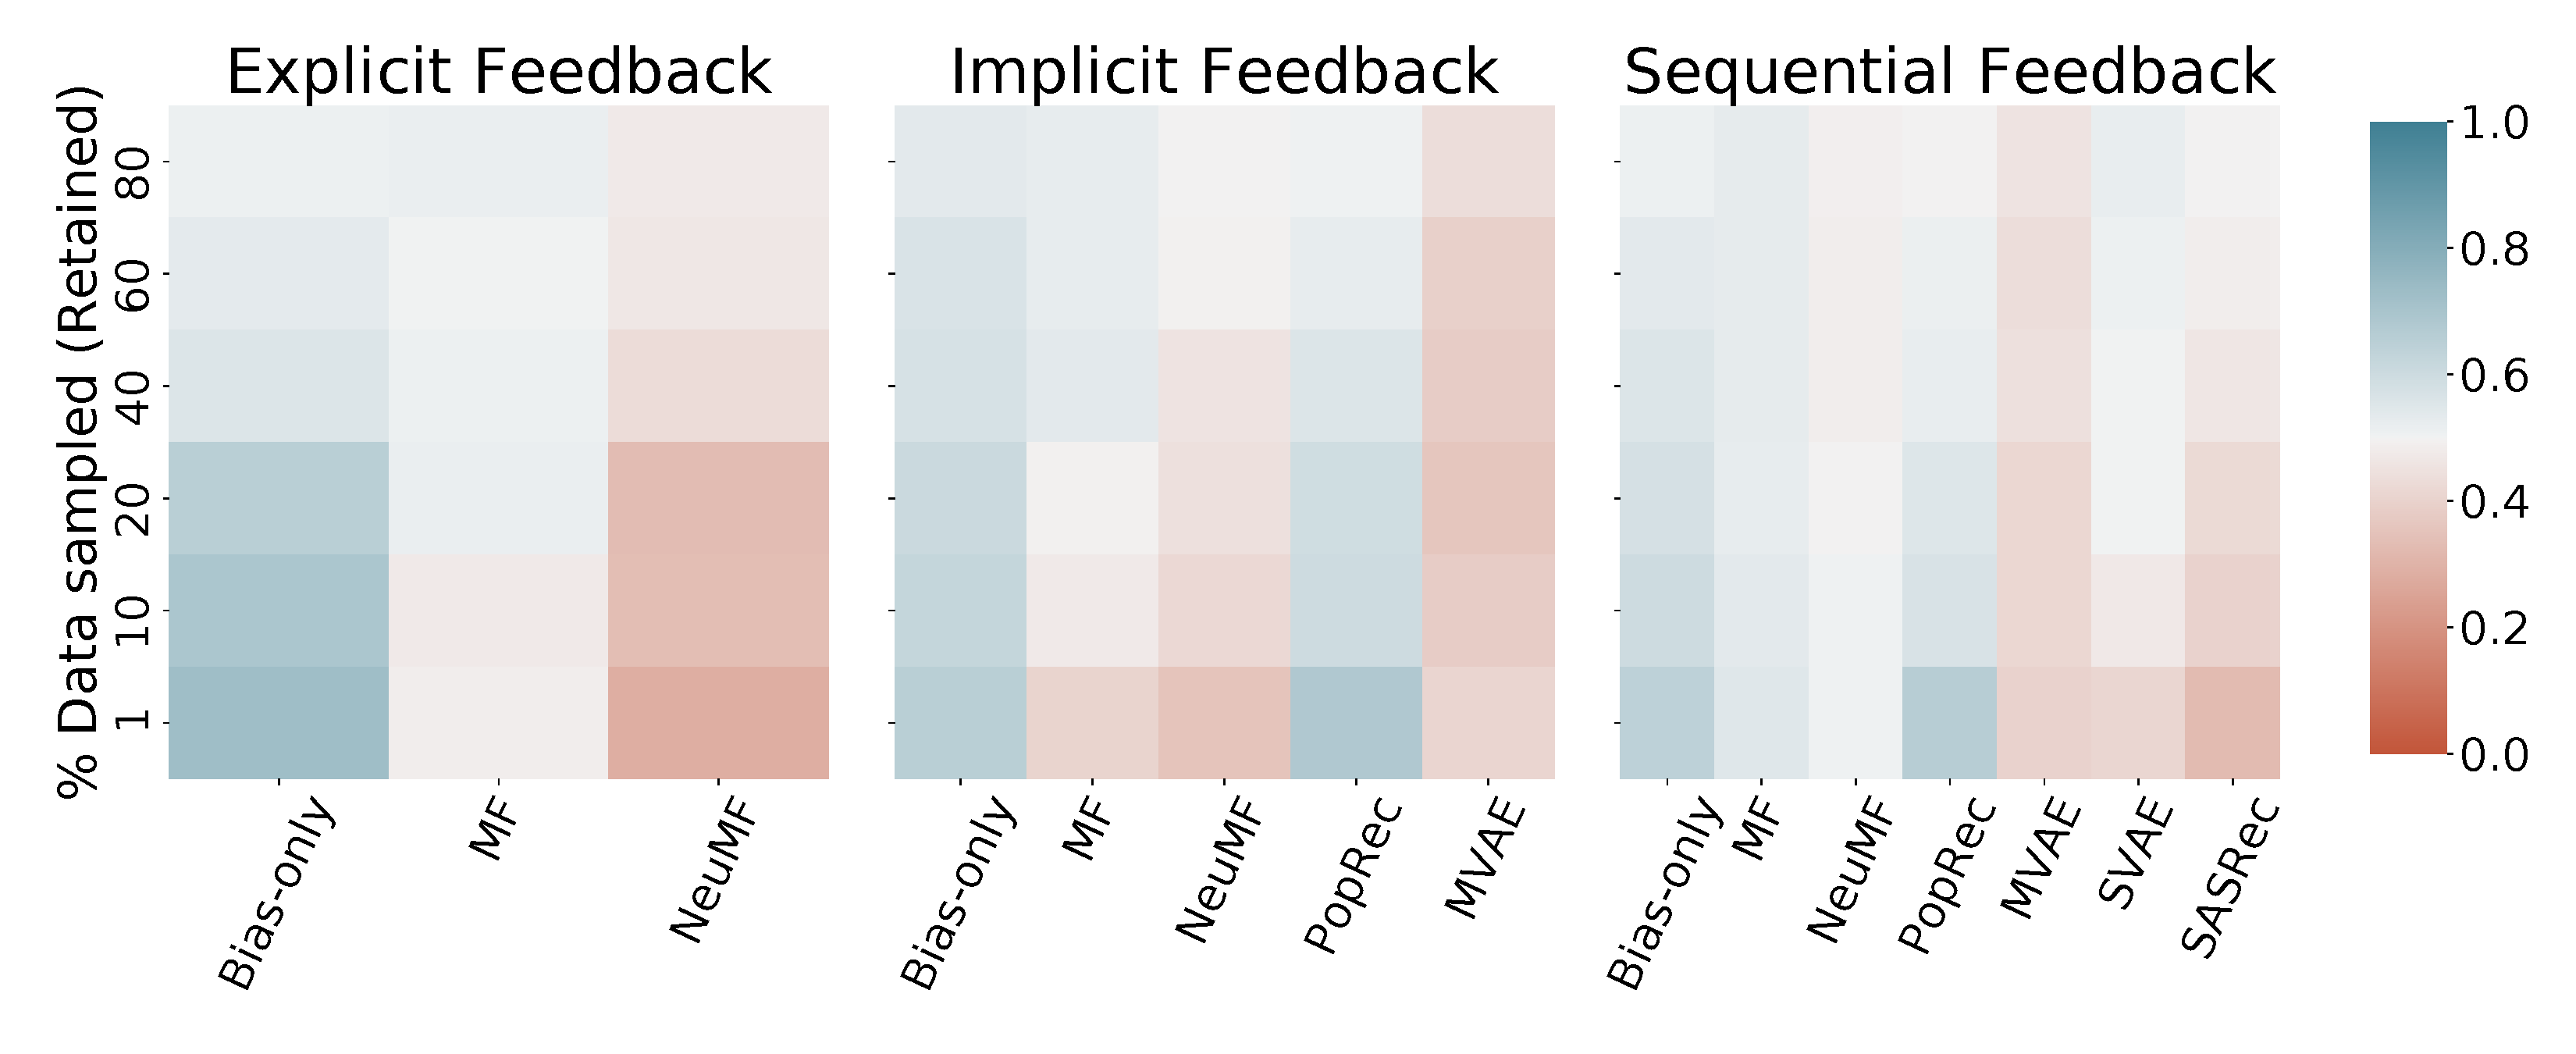
\includegraphics[width=0.9\linewidth]{figures/percent_sampling_vs_method.pdf}
    \vspace{-0.4cm}
    \caption{Heatmap of the probability of an algorithm moving in the overall ranking with extreme sampling. A high value indicates that the algorithm is most probable to \emph{move up} in the sampled data ranking order, whereas a low value indicates that the algorithm is most probable to \emph{move down}.}
    \label{percent_sampling_vs_method}
    \vspace{-0.3cm}
\end{figure}

\subsubsection{How much data to sample? \ \ } Since $\Psi$ is averaged over all $p \in \{ 80, 60, 40, 20, 10, 1 \}$\% data samples, to better estimate a reasonable amount of data to sample, we stratify $\Psi$ according to each value of $p$ and note the average Kendall's Tau. As we observe from \cref{percent_sampling_vs_tau}, %there is an expected, 
there is a steady increase in the performance measure when more data is retained. Next, despite the results in \cref{percent_sampling_vs_tau} being averaged over \emph{sixteen} sampling strategies, we still notice a significant amount of performance retained after sampling just $50-60\%$ of the data. % This holds to show that sampled data in some conditions can accurately reflect true algorithm performance.
\begin{figure}[ht!] 
    \centering
    \vspace{-0.2cm}
    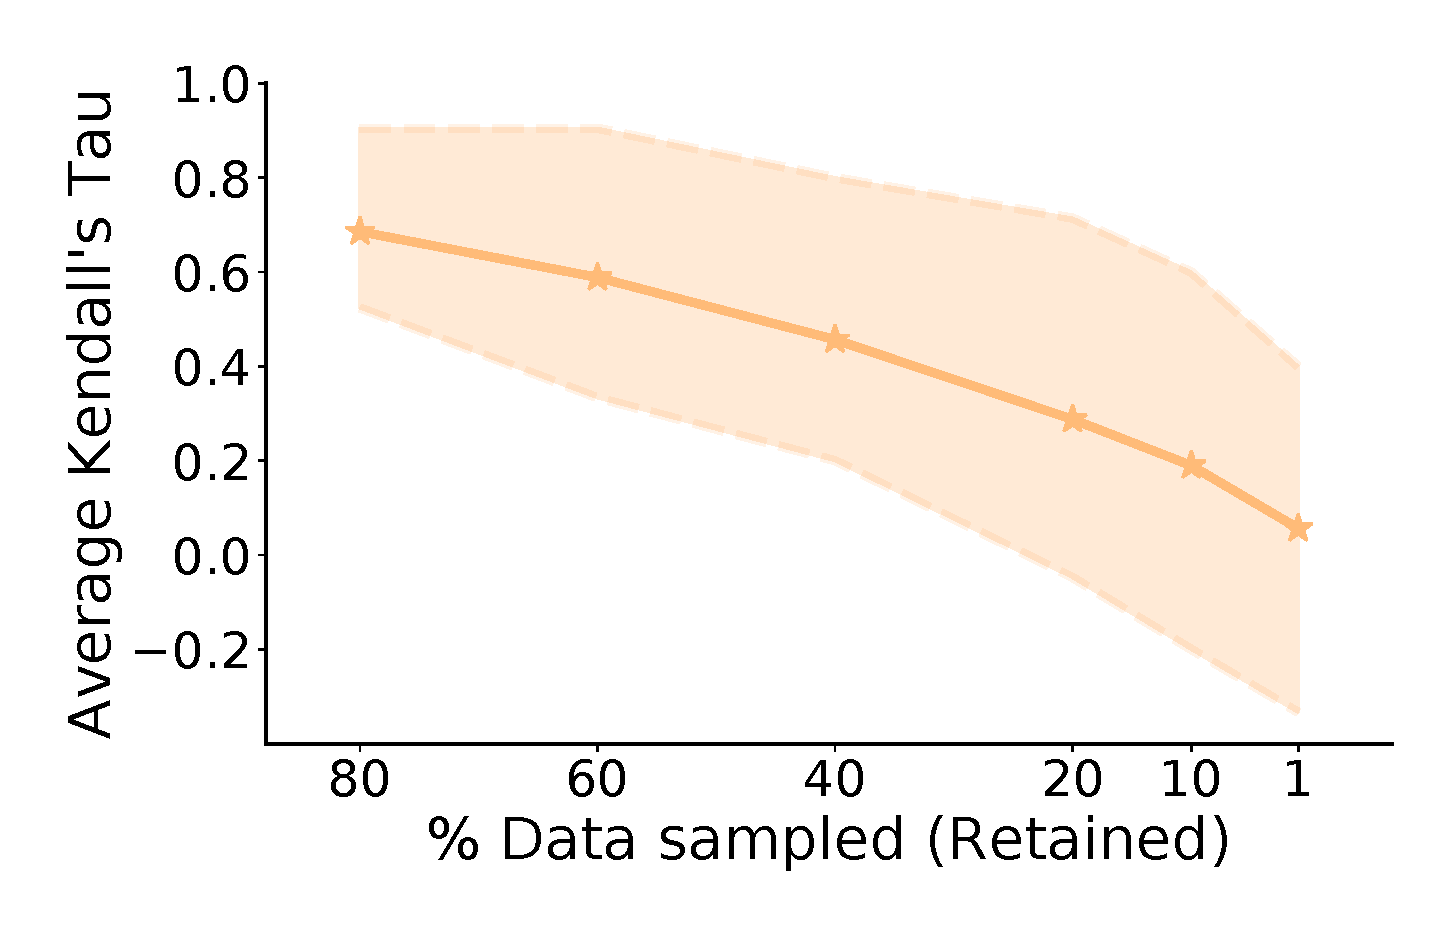
\includegraphics[width=0.6\linewidth]{figures/percent_sampling_vs_tau.pdf}
    \vspace{-0.25cm}
    \caption{Comparison of the average Kendall's Tau with \% data sampled. A higher Tau indicates better retaining power of the ranking of different recommendation algorithms.}
    \label{percent_sampling_vs_tau}
    \vspace{-0.3cm}
\end{figure} 

\subsubsection{Are different metrics affected equally by sampling? \ \ } In an attempt to better understand how the different implicit and sequential feedback metrics (\cref{feedback_types}) are affected by sampling, we visualize the average Kendall's Tau for all sampling strategies (except \sampler for brevity) and all \% data sampling choices separately over the AUC, Recall, and nDCG metrics in \cref{metric_correlation}. As expected, we observe a steady decrease in the model quality across the accuracy metrics over the different sampling schemes. This is in agreement with the analysis from \cref{percent_sampling_vs_tau}. Next, most sampling schemes follow a \emph{similar} downwards trend in performance for the three metrics with AUC being slightly less affected and nDCG being slightly more affected by extreme sampling.
\begin{figure}[ht!] 
    \vspace{-0.1cm}
    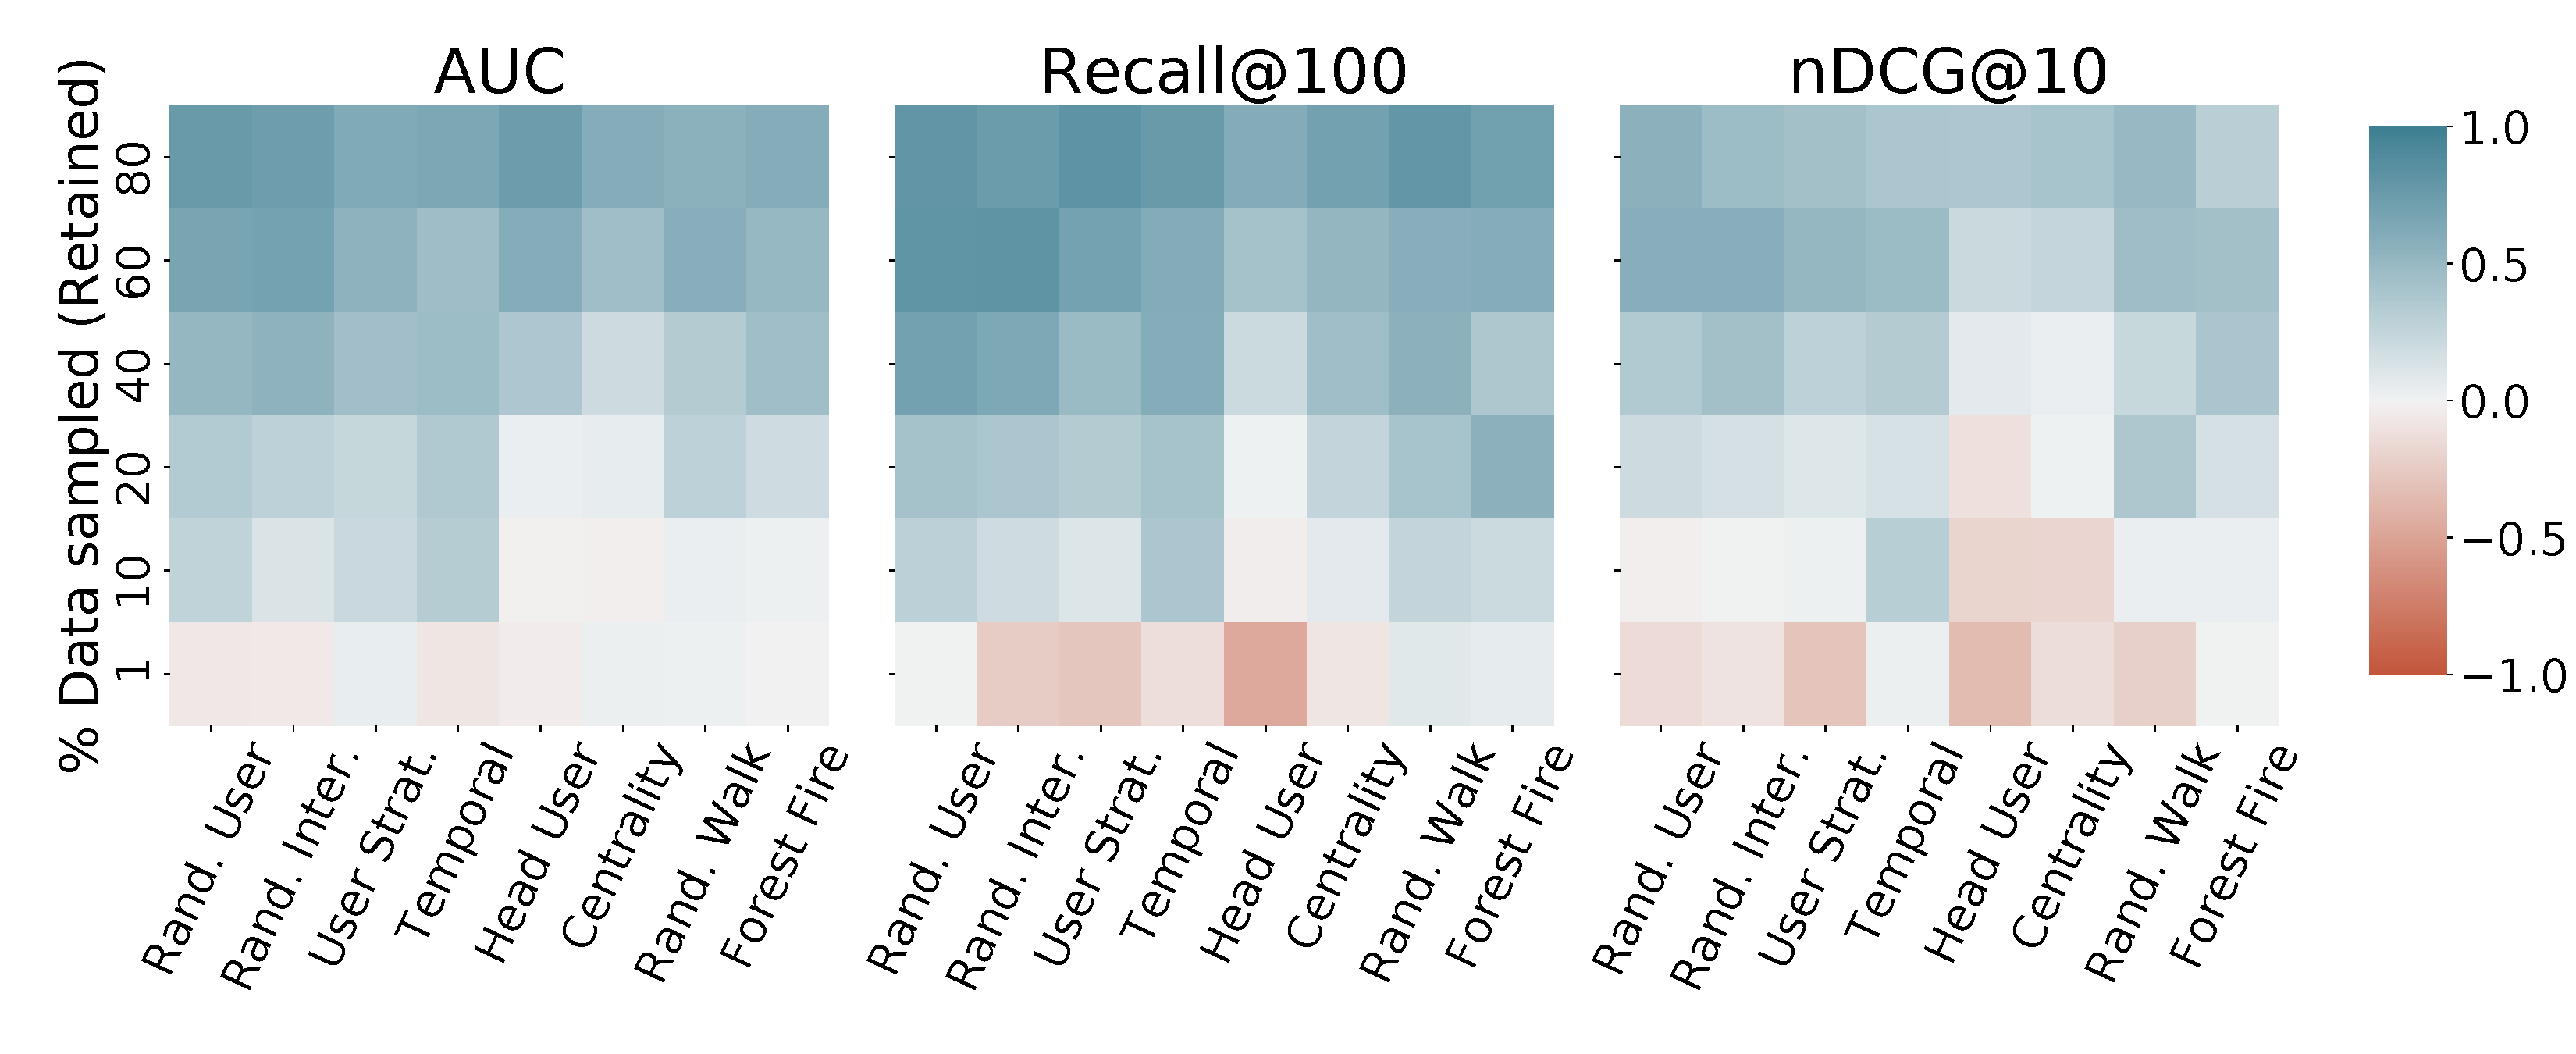
\includegraphics[width=\linewidth]{figures/percent_sampling_vs_sampler.pdf}
    \vspace{-0.8cm}
    \caption{Heatmap of the average Kendall's Tau for different samplers stratified over metrics and \% data sampled.}
    \label{metric_correlation}
    \vspace{-0.5cm}
\end{figure}
% \begin{wrapfigure}{r}{0.36\textwidth}
%     \vspace{-0.3cm}
%     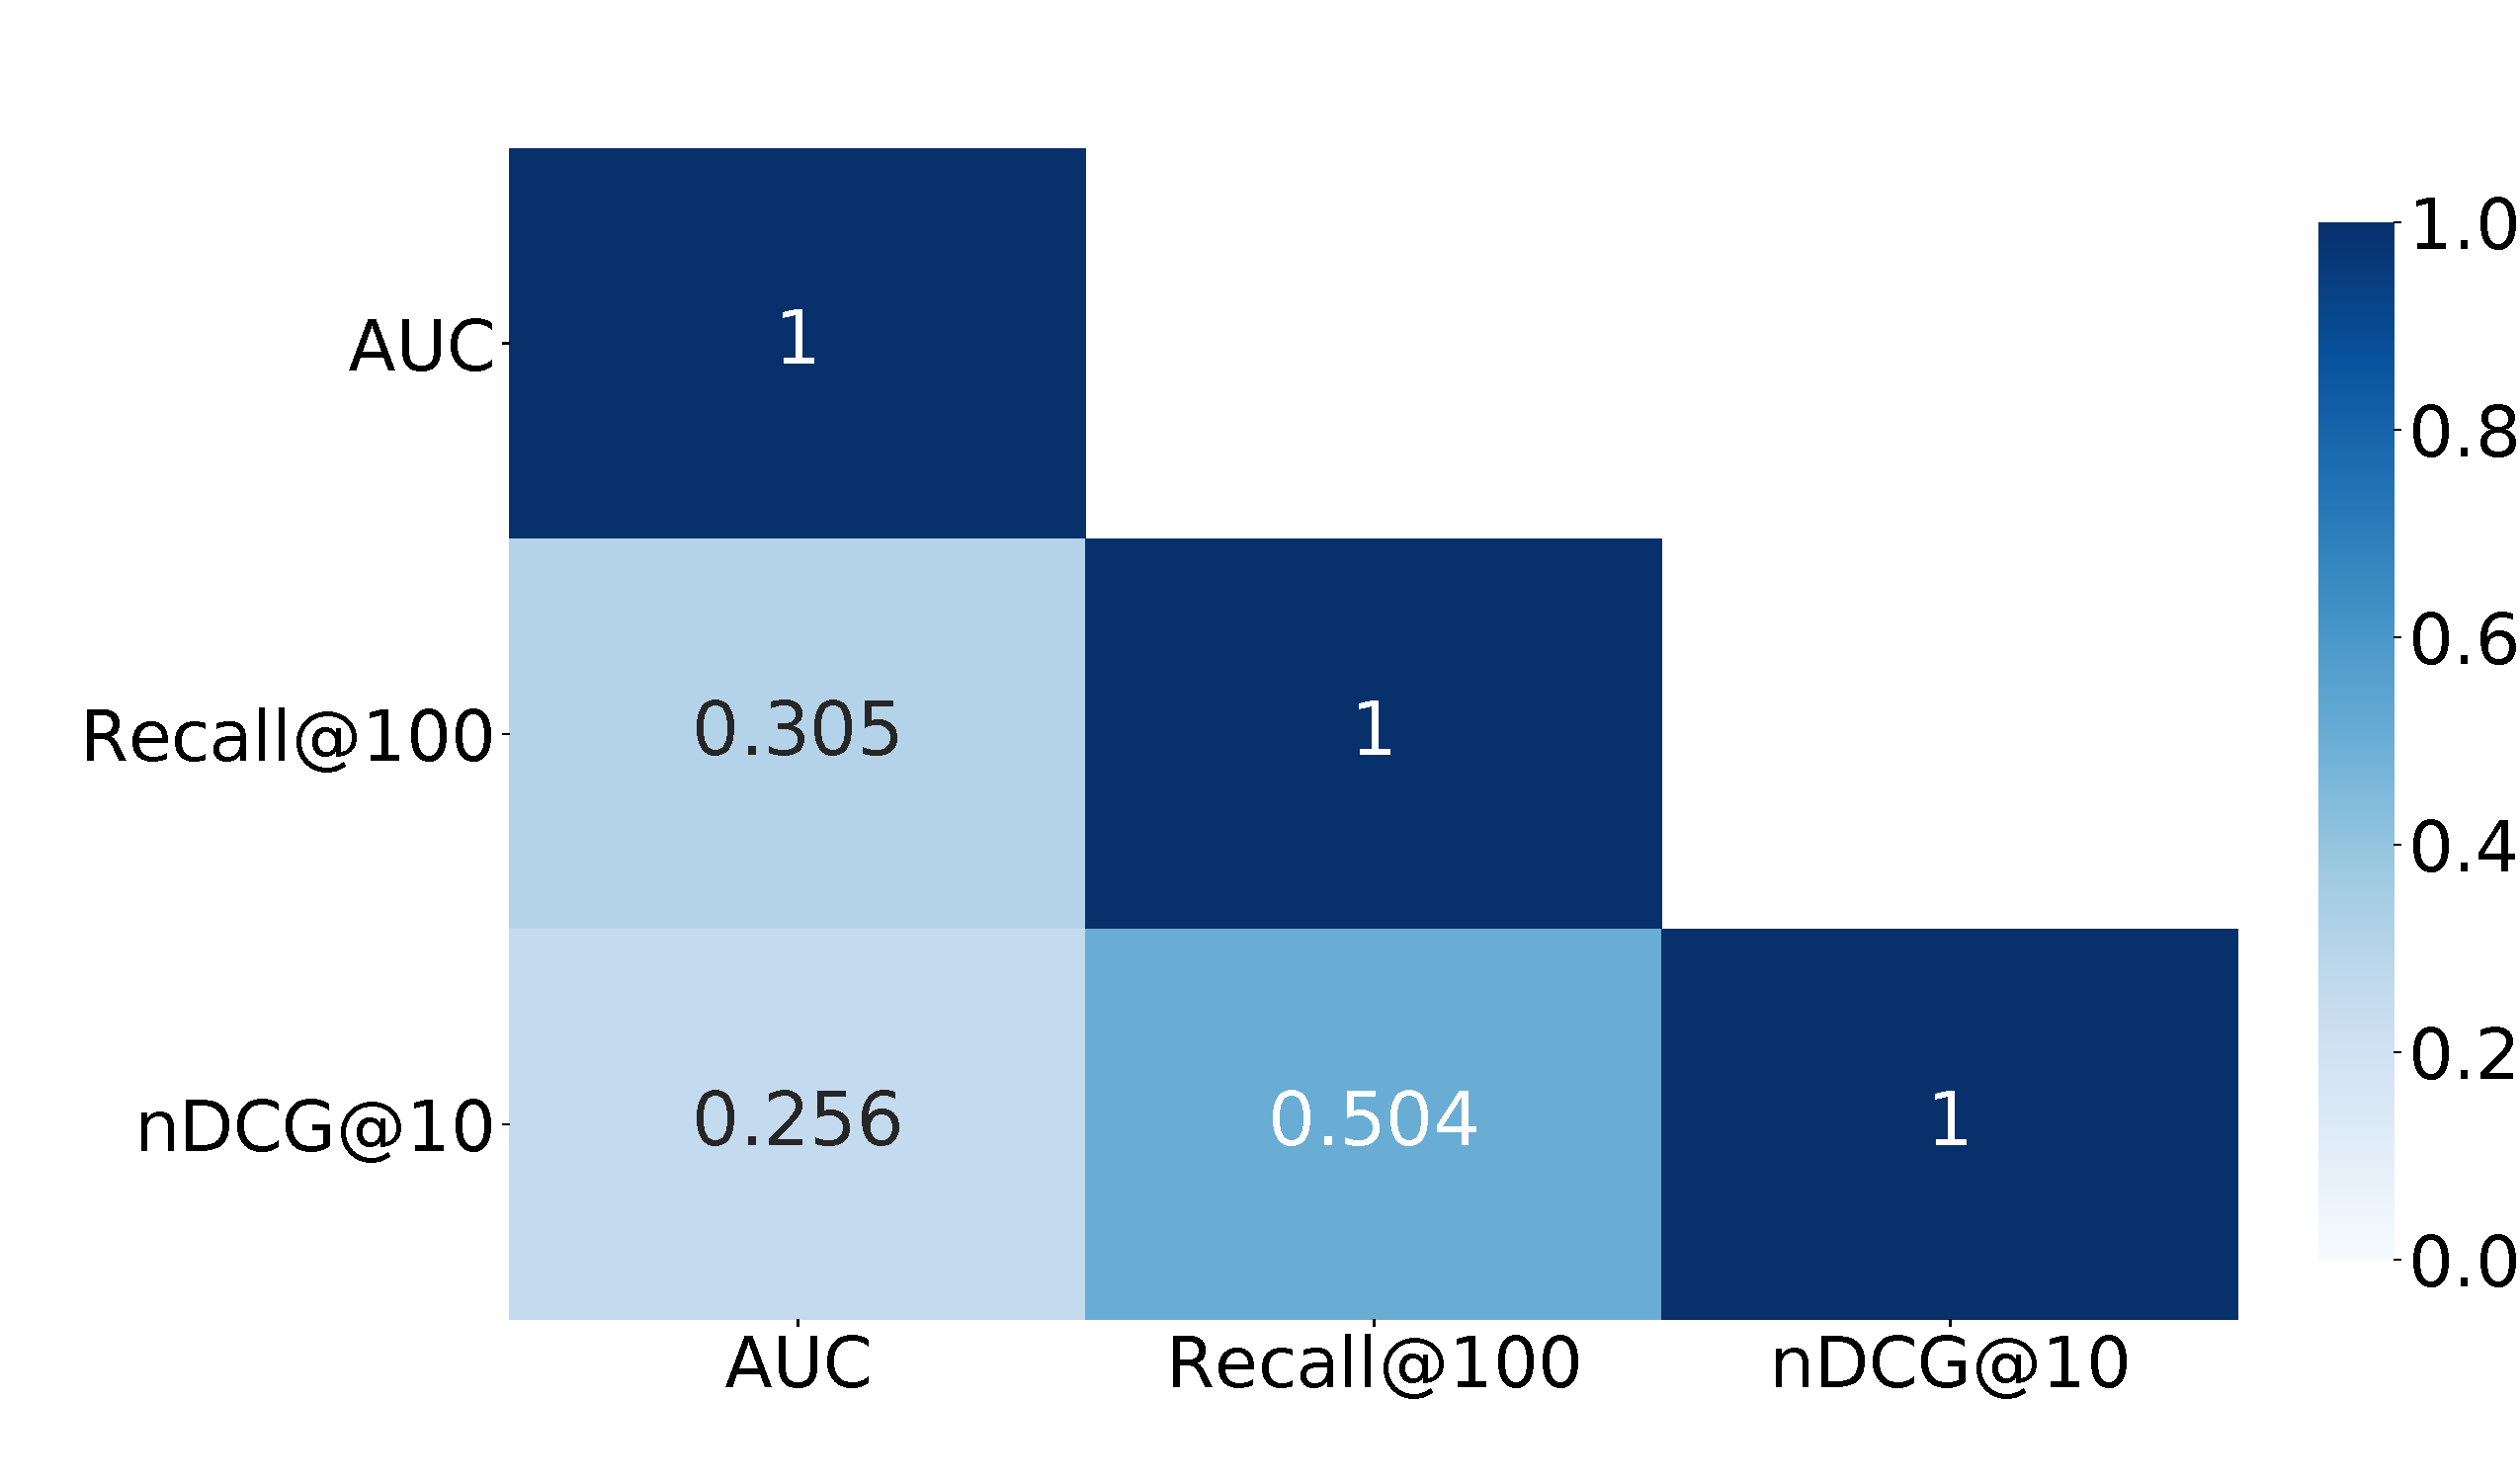
\includegraphics[width=\linewidth]{figures/metric_correlation.pdf}
%     \vspace{-0.92cm}
%     \caption{Average Kendall's Tau amongst the rankings of algorithms over different metrics.}
%     \label{metric_correlation}
%     \vspace{-0.5cm}
% \end{wrapfigure}
% \subsubsection{How do different metrics correlate with each other? \ \ } \ns{Check if we need to change this figure.} In an attempt to better understand how well do the three different implicit and sequential feedback metrics (\cref{feedback_types}) agree with each other, we visualize the average correlation between the algorithm rankings for each metric pair in \cref{metric_correlation}. To be precise, we compute the correlation between metric$_1$ and metric$_2$ as the Kendall's Tau between the ranked list of algorithms on metric$_1$ and metric$_2$ averaged over all datasets, sampling strategies and \% data sampled. We first observe that all three metrics correlate positively with each other. Finally, the AUC metric correlates less significantly with both Recall and nDCG than the correlation amongst Recall and nDCG.
% \begin{table}[!ht]
    % \vspace{0.05cm}
    \begin{footnotesize} % normalsize, small, footnotesize
    \begin{center}
        \begin{tabular}{c c | c c c}
            \toprule
            $\mathcal{E}$ & $\Phi$ & \textbf{MSE} & \textbf{P@1} \\ \midrule
            
            \multicolumn{2}{c|}{Random} & 0.2336 & 25.2 \\ 
            \multicolumn{2}{c|}{User sampling \emph{w/} Bias-only \samplerprop} & -- & 30.6 \\ \midrule
            
            Handcrafted & Least squares regression & 0.1866 & 31.7 \\
            '' & XGBoost regression & 0.1163 & 43.9 \\
            '' & \oracle-regression & \underline{0.1008} & 51.2 \\ 
            '' & \oracle-ranking    & -- & 51.2 \\ \midrule
            
            Unsupervised GCN & Least squares regression & 0.1838 & 39.1 \\
            '' & XGBoost regression & 0.1231 & 43.9 \\
            '' & \oracle-regression & 0.1293 & 48.8 \\ 
            '' & \oracle-ranking    & -- & \underline{53.7} \\ \bottomrule
        \end{tabular}
    \end{center}
    \end{footnotesize}
    \vspace{0.5cm}
    \caption{Results for predicting the best sampling scheme for a particular dataset over a germane metric. The MSE-value next to randomly choosing the sampling scheme represents the variance of the test-set. Best values are \underline{underlined}.}
    \label{oracle_results}
    \vspace{-6mm} %Put here to reduce too much white space after your table
% \end{table}
\newcommand{\dataset}[0]{$\mathcal{D}$\xspace}
\newcommand{\sampled}[0]{$\mathcal{D}'$\xspace}
\newcommand{\argmin}[1]{\underset{#1}{\operatorname{arg}\,\operatorname{min}}\;}

\newcommand{\oracle}{\textsc{Data-genie}\xspace}
\newcommand{\sampler}{\textsc{SVP-CF}\xspace}
\newcommand{\samplerprop}{\textsc{SVP-CF-Prop}\xspace}

\newcommand{\EE}{\operatornamewithlimits{\mathbb{E}}} % Expectation
\paragraph{Sampling CF data.} Sampling in CF-data has been a popular choice for three major scenarios. Most prominently, sampling is used for mining hard-negatives while training recommendation algorithms. Some popular approaches include random sampling; using the graph-structure % to find the hardest negatives 
\cite{pinsage, eclare}; and ad-hoc techniques like similarity search \cite{slice}, stratified sampling \cite{sampling_cf_nn}, \etc % On the other hand, 
Sampling is also generally employed for evaluating recommendation algorithms by estimating expensive to compute metrics like Recall, nDCG, \etc \cite{sampled_metrics, castells_sampling}. Finally, sampling is also used to create smaller sub-samples of 
% the \emph{entire} data 
a big dataset
for reasons like fast experimentation, benchmarking different algorithms, privacy concerns, \etc However, the consequences of different samplers on any of these downstream applications is under-studied, and is the main research interest of this paper. 

\paragraph{Coreset selection.} Closest to our work, a coreset is loosely defined as a subset of data-points that maintains a similar ``quality'' as the full dataset for subsequent model training. Submodular approaches try to optimize a function $f : \mathbf{V} \mapsto \mathcal{R}_+$ which measures the utility of a subset $\mathbf{V} \subseteq \mathbf{X}$, and use it as a proxy to select the best coreset \cite{coreset_1}. More recent works treat coreset selection as a bi-level optimization problem \cite{coreset_bilevel, coreset_bilevel_2} and directly optimize for the best coreset for a given downstream task. Selection-via-proxy \cite{svp} is another technique which employs a base-model as a proxy to tag the importance of each data-point. Note, however, that 
% all of the discussed 
most existing
coreset selection approaches were designed primarily for classification data, whereas adapting them for CF-data is non-trivial because of: (1) the inherent data heterogeneity; the (2) wide range of recommendation metrics; and (3) the prevalent missing-data characteristics.

\paragraph{Evaluating sample quality.} The quality of a dataset sample, if estimated correctly is of high interest for various applications. Short of being able to evaluate the ``true'' utility of a sample, one generally resorts to either retaining task-dependent characteristics \cite{evaluate_sample_quality_1} \emph{or} employing universal, handcrafted features like a social network's hop distribution, eigenvalue distribution, \etc \cite{large_graphs} as meaningful proxies. Note that evaluating the sample quality with a limited set of handcrafted features might introduce bias in the sampled data, depending on the number and quality of such features.

% Brief motivation as to why we need this paper
Representative \emph{sampling} of collaborative filtering (CF) data is a crucial problem from numerous stand-points and can be performed at various levels: (1) mining hard-negatives while training complex algorithms over massive datasets \cite{eclare, sampling_cf_nn}; (2) down-sampling the item-space to estimate expensive ranking metrics \cite{sampled_metrics, castells_sampling}; and (3) 
% sub-sampling the entire dataset for 
reasons like easy-sharing, fast-experimentation, mitigating the significant environmental footprint of training resource-hungry machine learning models \cite{google_emissions, wu2021sustainable, facebook_emissions, green_ai}. In this paper, we are interested in finding a sub-sample of a dataset which has minimal effects on model utility evaluation \ie an algorithm performing well on the sub-sample should also perform well on the original dataset.

Preserving \emph{exactly} the same levels of performance on sub-sampled data over metrics, such as MSE and AUC, is a challenging problem. A simpler yet useful problem is accurately preserving the \emph{ranking} or relative performance of different algorithms on sub-sampled data. For example, a sampling scheme that has low bias but high variance in preserving metric performance values has less utility than a different sampling scheme with high amounts of bias but low variance, since the overall algorithm ranking is still preserved. 

% What wrong/good people have been doing
Performing 
% careless and 
ad-hoc sampling such as randomly removing interactions, or making dense subsets by removing users \emph{or} items with few interactions \cite{sigir20} can have adverse downstream repercussions. For example, sampling only the head-portion of a dataset---from a fairness and inclusion perspective---is inherently biased against minority-groups and benchmarking algorithms on this biased data is 
% highly 
likely to propagate the 
% original sampling biases. 
original sampling bias.
% On the other hand, 
Alternatively,
simply from 
% the model quality performance view-point, 
a model performance view-point,
accurately retaining the relative performance of different recommendation algorithms on much smaller sub-samples is a challenging research problem in itself.

% What do we actually do in this paper?
Two prominent directions toward better and more representative sampling of CF data are: (1) designing principled sampling strategies, especially for user-item interaction data; and (2) analyzing the performance of different sampling strategies, in order to better grasp which sampling scheme performs ``better'' for which types of data. \emph{In this paper,} we explore both directions through the lens of expediting the recommendation algorithm development cycle by:
\begin{itemize}
    \item Characterizing the efficacy of \emph{sixteen} different sampling strategies in accurately benchmarking various kinds of recommendation algorithms on smaller sub-samples.

    \item Proposing a sampling strategy, \sampler, which dynamically samples the ``toughest'' portion of a CF dataset. \sampler is tailor-designed to handle the inherent data heterogeneity and missing-not-at-random properties in user-item interaction data.
    
    \item Developing \oracle, which analyzes the \emph{performance} of different sampling strategies. Given a dataset sub-sample, \oracle can directly estimate the likelihood of model performance being preserved on that sample. 
\end{itemize}
%
% Give a taste of the findings.
Ultimately, our experiments reveal that \sampler outperforms all other sampling strategies and can accurately benchmark recommendation algorithms with roughly $50-60\%$ of the original dataset size. Furthermore, by employing \oracle to dynamically select the best sampling scheme for a dataset, we are able to preserve model performance with only $10\%$ of the initial data, leading to a net $5.8\times$ training time speedup.

\begin{table*}[!ht]
    \begin{small} % normalsize, small, footnotesize
    \begin{center}
        % \begin{subtable}{0.5\linewidth}
        % \centering
        %     \begin{tabular}{c | c c c}
        %         \toprule
        %         \multirow{2}{*}{Algorithm} & \multicolumn{3}{c}{CF-scenario} \\
        %         & Explicit & Implicit & Sequential \\ \midrule
                
        %         Bias-only   & Yes & Yes & Yes \\
        %         MF          & Yes & Yes & Yes \\
        %         NeuMF       & Yes & Yes & Yes \\
        %         PopRec      & $\times$ & Yes & Yes \\
        %         MVAE        & $\times$ & Yes & Yes \\
        %         SVAE        & $\times$ & $\times$ & Yes \\
        %         SASRec      & $\times$ & $\times$ & Yes \\ \bottomrule
        %     \end{tabular}
        % \end{subtable}%
        % \begin{subtable}{0.5\linewidth}
        % \centering
        %     \begin{tabular}{c | c c c}
        %         \toprule
        %         \multirow{2}{*}{Metric} & \multicolumn{3}{c}{CF-scenario} \\
        %         & Explicit & Implicit & Sequential \\ \midrule
                
        %         MSE       & Yes & $\times$ & $\times$ \\
        %         AUC       & $\times$ & Yes & Yes \\
        %         Recall@k  & $\times$ & Yes & Yes \\
        %         nDCG@k    & $\times$ & Yes & Yes \\ \bottomrule
        %     \end{tabular}
        % \end{subtable}%
        \begin{tabular}{c | c c c c c c c | c c c c}
            \toprule
            \multirow{3}{*}{CF-scenario} & \multicolumn{7}{c|}{\emph{Algorithm}} & \multicolumn{4}{c}{\emph{Metric}} \\
            & \multicolumn{7}{c|}{} & \multicolumn{4}{c}{} \\
            & Bias-only & MF & NeuMF & PopRec & MVAE & SVAE & SASRec & MSE & AUC & Recall@k & nDCG@k \\ \midrule
            Explicit & Yes & Yes & Yes & $\times$ & $\times$ & $\times$ & $\times$ & Yes & $\times$ & $\times$ & $\times$ \\[0.6mm]
            Implicit & Yes & Yes & Yes & Yes & Yes & $\times$ & $\times$ & $\times$ & Yes & Yes & Yes \\[0.6mm]
            Sequential & Yes & Yes & Yes & Yes & Yes & Yes & Yes & $\times$ & Yes & Yes & Yes \\[0.6mm]
            \bottomrule
        \end{tabular}
    \end{center}
    \end{small}
    \bigskip
    \caption{Demonstrates the pertinence of each CF-scenario towards each algorithm (left) and each metric (right). Note that we can use ranking metrics for explicit feedback, however, we only use MSE as a design choice and due to it's direct relevance.}
    \label{model_scenario_table}
    \vspace{-6mm} %Put here to reduce too much white space after your table
\end{table*}
% \makeatletter \renewcommand\paragraph{\@startsection{paragraph}{4}{\z@} {2mm \@plus1ex \@minus.2ex} {-0.7em} {\normalfont\normalsize\bfseries}} \makeatother
\makeatletter \renewcommand\paragraph{\@startsection{paragraph}{4}{\z@} {2mm \@plus1ex \@minus.2ex} {-0.7em} {\normalfont\normalsize\itshape}} \makeatother

\newcommand{\listheader}[1]{\item \emph{#1} }

\newcommand\overstar[1]{\ThisStyle{\ensurestackMath{%
  \setbox0=\hbox{$\SavedStyle#1$}%
  \stackengine{0pt}{\copy0}{\kern.2\ht0\smash{\SavedStyle*}}{O}{c}{F}{T}{S}}}}

\newtheorem{theorem}{Theorem}[section]
\newtheorem{lemma}[theorem]{Lemma}
\newtheorem{proposition}[theorem]{Proposition}

\newcommand{\bs}[1]{\ensuremath{\bm{\mathit{#1}}}}

\newcommand{\ns}[1]{\textcolor{blue}{[Noveen: #1]}}
\newcommand{\jm}[1]{\textcolor{purple}{[Julian: #1]}}
\newcommand{\ie}[0]{\emph{i.e.}\xspace}
\newcommand{\etc}[0]{\emph{etc.}\xspace}
\newcommand{\eg}[0]{\emph{e.g.}\xspace}
\newcommand{\vs}[0]{\emph{vs.}\xspace}
\newcommand{\wrt}[0]{\emph{w.r.t.}\xspace}

